%%% SystsUncer %%%
\label{ch:SystsUncer}

%These systematic variations are estimated on the final discriminant.
This chapter describes the sources of systematic uncertainties considered in the analysis, divided into three categories: experimental uncertainties, uncertainties on the modelling of background processes, and theoretical uncertainties on the signal processes. In the statistical analysis, each systematic uncertainty is treated as a nuisance parameter (NP); the names of these parameters are defined below. 
Unless specified, these NPs are included in the final binned maximum likelihood fit, which will be discussed further in Chapter~\ref{ch:stat_interpretation}.

%
\section{Experimental Uncertainties}
%\subsection{Experimental Uncertainties}
\label{subsec:exp_uncer}


\subsection{Baseline uncertainties}
\label{subsubsec:baseline_unc}
The summary of experimental uncertainties is presented in Tab.~\ref{tab:syst_summary_sources_1} to \ref{tab:syst_summary_sources_3}.
 
\begin{table}[!hp]
  \caption{ Qualitative summary of the systematic uncertainties included in this analysis. }
  \label{tab:syst_summary_sources_1}
  \centering
  \footnotesize
  \begin{center}
    \begin{tabular}{|l|l|l|l|}
      \hline
      Source        & Description                     & Analysis Name                         & Notes              \\ \hline
      Electrons     & Energy scale                    &  EG\_SCALE\_ALL                     & \\ 
      Electrons     & Energy resolution               &  EG\_RESOLUTION\_ALL                & \\ 
      Electrons     & Trigger                        &  EL\_EFF\_Trigger\_TOTAL\_1NPCOR\_PLUS\_UNCOR                    & \\ 
      Electrons     & ID efficiency SF                &  EL\_EFF\_ID\_TOTAL\_1NPCOR\_PLUS\_UNCOR  & \\
      Electrons     & Isolation efficiency SF                &   EL\_EFF\_Iso\_TOTAL\_1NPCOR\_PLUS\_UNCOR  & \\
      Electrons     & Reconstruction efficiency SF                &   EL\_EFF\_Reco\_TOTAL\_1NPCOR\_PLUS\_UNCOR  & \\ \hline
      Muons         & \pt\ scale                       &   MUONS\_SCALE                       & \\ 
      Muons         & \pt\ scale (charge dependent)          &   MUON\_SAGITTA\_RHO                    & \\ 
      Muons         & \pt\ scale (charge dependent)          &   MUON\_SAGITTA\_RESBIAS                     & \\ 
      Muons         & \pt\ resolution MS               &   MUONS\_MS                          & \\ 
      Muons         & \pt\ resolution ID               &   MUONS\_ID                          & \\ 
      Muons         & Isolation efficiency SF         &   MUON\_ISO\_SYS                     & \\ 
      Muons         & Isolation efficiency SF         &   MUON\_ISO\_STAT                    & \\ 
      Muons         & Muon reco \& ID efficiency SF               &   MUONS\_EFF\_STAT                          & \\ 
      Muons         & Muon reco \& ID efficiency SF               &   MUONS\_EFF\_STAT\_LOWPT                          & \\ 
      Muons         & Muon reco \& ID efficiency SF               &   MUONS\_EFF\_SYST                          & \\ 
      Muons         & Muon reco \& ID efficiency SF               &   MUONS\_EFF\_SYST\_LOWPT                          & \\ 
      Muons         & Track-to-vertex association efficiency SF         &   MUON\_TTVA\_SYS                     & \\ 
      Muons         & Track-to-vertex association efficiency SF         &   MUON\_TTVA\_STAT                     & \\ 
      Muons         & Trigger         &   MUON\_EFF\_TrigSystUncertainty   & \\
      Muons         & Trigger         &   MUON\_EFF\_TrigStatUncertainty   & \\    \hline
        %MET           & Trigger scale factor            &   METTrigStat                        & \\
        %MET           & Trigger scale factor            &   METTrigTop                         & \\
      MET           & Soft term                       &   MET\_SoftTrk\_ResoPerp             & \\ 
      MET           & Soft term                       &   MET\_SoftTrk\_ResoPara             & \\ 
      MET           & Soft term                       &   MET\_SoftTrk\_Scale              & \\
      %MET           & Jet track uncertainties         &   MET\_JetTrk\_Scale                 & \\ 
      \hline
      \end{tabular}
    \end{center}
  \end{table}

%\textcolor{red}{cross-check with latest fit inputs}

\begin{table}[!hp]
  \caption{ Qualitative summary of the systematic uncertainties included in this analysis. }
  \label{tab:syst_summary_sources_2}
  \centering
  \footnotesize
  \begin{center}
    \begin{tabular}{|l|l|l|l|}
      \hline
      Source        & Description                     & Analysis Name                         & Notes              \\ \hline
      Small-R Jets  & JES category reduction            &  JET\_CR\_JET\_BJES\_Response                             & \\ 
      Small-R Jets  & JES category reduction            &  JET\_CR\_JET\_EffectiveNP\_Detector1                     & \\ 
      Small-R Jets  & JES category reduction            &  JET\_CR\_JET\_EffectiveNP\_Detector2                     & \\ 
      Small-R Jets  & JES category reduction            &  JET\_CR\_JET\_EffectiveNP\_Mixed1                        & \\ 
      Small-R Jets  & JES category reduction            &  JET\_CR\_JET\_EffectiveNP\_Mixed2                        & \\ 
      Small-R Jets  & JES category reduction            &  JET\_CR\_JET\_EffectiveNP\_Mixed3                        & \\ 
      Small-R Jets  & JES category reduction            &  JET\_CR\_JET\_EffectiveNP\_Modelling1                    & \\ 
      Small-R Jets  & JES category reduction            &  JET\_CR\_JET\_EffectiveNP\_Modelling2                    & \\ 
      Small-R Jets  & JES category reduction            &  JET\_CR\_JET\_EffectiveNP\_Modelling3                    & \\ 
      Small-R Jets  & JES category reduction            &  JET\_CR\_JET\_EffectiveNP\_Modelling4                    & \\ 
      Small-R Jets  & JES category reduction            &  JET\_CR\_JET\_EffectiveNP\_Statistical1                  & \\ 
      Small-R Jets  & JES category reduction            &  JET\_CR\_JET\_EffectiveNP\_Statistical2                  & \\ 
      Small-R Jets  & JES category reduction            &  JET\_CR\_JET\_EffectiveNP\_Statistical3                  & \\ 
      Small-R Jets  & JES category reduction            &  JET\_CR\_JET\_EffectiveNP\_Statistical4                  & \\ 
      Small-R Jets  & JES category reduction            &  JET\_CR\_JET\_EffectiveNP\_Statistical5                  & \\ 
      Small-R Jets  & JES category reduction            &  JET\_CR\_JET\_EffectiveNP\_Statistical6                  & \\ 
      Small-R Jets  & JES category reduction            &  JET\_CR\_JET\_Flavor\_Composition                        & \\ 
      Small-R Jets  & JES category reduction            &  JET\_CR\_JET\_Flavor\_Response                           & \\ 
      Small-R Jets  & JES category reduction            &  JET\_CR\_JET\_Pileup\_OffsetMu                           & \\ 
      Small-R Jets  & JES category reduction            &  JET\_CR\_JET\_Pileup\_OffsetNPV                          & \\ 
      Small-R Jets  & JES category reduction            &  JET\_CR\_JET\_Pileup\_PtTerm                             & \\ 
      Small-R Jets  & JES category reduction            &  JET\_CR\_JET\_Pileup\_RhoTopology                        & \\ 
      Small-R Jets  & JES category reduction            &  JET\_CR\_JET\_PunchThrough\_MC16                         & \\ 
      Small-R Jets  & JES category reduction            &  JET\_CR\_JET\_SingleParticle\_HighPt                     & \\ 
      Small-R Jets  & JES category reduction            &  JET\_CR\_JET\_EtaIntercalibration\_TotalStat             & \\ 
      Small-R Jets  & JES category reduction            &  JET\_CR\_JET\_EtaIntercalibration\_Modelling             & \\ 
      Small-R Jets  & JES category reduction            &  JET\_CR\_JET\_EtaIntercalibration\_NonClosure\_highE     & \\ 
      Small-R Jets  & JES category reduction            &  JET\_CR\_JET\_EtaIntercalibration\_NonClosure\_negEta    & \\ 
      Small-R Jets  & JES category reduction            &  JET\_CR\_JET\_EtaIntercalibration\_NonClosure\_posEta    & \\ 
        \hline
        Small-R Jets  & JER                  &  JET\_CR\_JET\_JER\_DataVsMC                  & \\ 
        Small-R Jets  & JER                  &  JET\_CR\_JET\_JER\_EffectiveNP\_1            & \\ 
        Small-R Jets  & JER                  &  JET\_CR\_JET\_JER\_EffectiveNP\_2            & \\ 
        Small-R Jets  & JER                  &  JET\_CR\_JET\_JER\_EffectiveNP\_3            & \\ 
        Small-R Jets  & JER                  &  JET\_CR\_JET\_JER\_EffectiveNP\_4            & \\ 
        Small-R Jets  & JER                  &  JET\_CR\_JET\_JER\_EffectiveNP\_5            & \\ 
        Small-R Jets  & JER                  &  JET\_CR\_JET\_JER\_EffectiveNP\_6            & \\ 
        Small-R Jets  & JER                  &  JET\_CR\_JET\_JER\_EffectiveNP\_7restTerm    & \\ 
        \hline
        Small-R Jets  & JVT                  &  JET\_JvtEfficiency    & \\
%        Small-R Jets  & fJVT                  &  JET\_fJvtEfficiency    & \\ 
        \hline
        \end{tabular}
    \end{center}
  \end{table}

%\textcolor{red}{cross-check with latest fit inputs}

\begin{table}[!hp]
  \caption{ Qualitative summary of the systematic uncertainties included in this analysis. }
  \label{tab:syst_summary_sources_3}
  \centering
  \footnotesize
  \begin{center}
    \begin{tabular}{|l|l|l|l|}
      \hline
      Source        & Description                     & Analysis Name                         & Notes              \\ \hline
      Large-R Jets  & \pt scale                       & FATJET\_Medium\_JET\_Rtrk\_Baseline\_pT                            &  \\
      %Large-R Jets  & \pt scale                       & FATJET\_Medium\_JET\_Rtrk\_Closure\_pT                             &  \\
      Large-R Jets  & \pt scale                       & FATJET\_Medium\_JET\_Rtrk\_Modelling\_pT                           &  \\
      Large-R Jets  & \pt scale                       & FATJET\_Medium\_JET\_Rtrk\_TotalStat\_pT                           &  \\
      Large-R Jets  & \pt scale                       & FATJET\_Medium\_JET\_Rtrk\_Tracking\_pT                            &  \\

      Large-R Jets  & \pt scale                       & FATJET\_BJT\_JET\_EtaIntercalibration\_Modelling      & \\
      Large-R Jets  & \pt scale                       & FATJET\_BJT\_JET\_Flavor\_Composition                 & \\
      Large-R Jets  & \pt scale                       & FATJET\_BJT\_JET\_Flavor\_Response                    & \\

      Large-R Jets  & Mass resolution                 & FATJET\_JMR                            & \\\hline
      Large-R Jets  & JER                             & FATJET\_JER                            & \\\hline

%
      B-tagging     & Flavor tagging scale factors    &  FT\_EFF\_Eigen\_B\_0\_AntiKt4PFlowJets                                & \\
      B-tagging     & Flavor tagging scale factors    &  FT\_EFF\_Eigen\_B\_1\_AntiKt4PFlowJets                                & \\
      B-tagging     & Flavor tagging scale factors    &  FT\_EFF\_Eigen\_B\_2\_AntiKt4PFlowJets                                & \\
      B-tagging     & Flavor tagging scale factors    &  FT\_EFF\_Eigen\_C\_0\_AntiKt4PFlowJets                                & \\
      B-tagging     & Flavor tagging scale factors    &  FT\_EFF\_Eigen\_C\_1\_AntiKt4PFlowJets                                & \\
      B-tagging     & Flavor tagging scale factors    &  FT\_EFF\_Eigen\_C\_2\_AntiKt4PFlowJets                                & \\
      B-tagging     & Flavor tagging scale factors    &  FT\_EFF\_Eigen\_C\_3\_AntiKt4PFlowJets                                & \\
      B-tagging     & Flavor tagging scale factors    &  FT\_EFF\_Eigen\_Light\_0\_AntiKt4PFlowJets                            & \\
      B-tagging     & Flavor tagging scale factors    &  FT\_EFF\_Eigen\_Light\_1\_AntiKt4PFlowJets                            & \\
      B-tagging     & Flavor tagging scale factors    &  FT\_EFF\_Eigen\_Light\_2\_AntiKt4PFlowJets                            & \\
      B-tagging     & Flavor tagging scale factors    &  FT\_EFF\_Eigen\_Light\_3\_AntiKt4PFlowJets                            & \\
      B-tagging     & Flavor tagging scale factors    &  FT\_EFF\_extrapolation\_AntiKt4PFlowJets                              & \\
      B-tagging     & Flavor tagging scale factors    &  FT\_EFF\_extrapolation\_from\_charm\_AntiKt4PFlowJets                 & \\

      \hline                          
      Pileup reweighting & PRW\_DATASF & PRW\_DATASF &\\ 
      Luminosity & LumiNP & ATLAS\_LUMI\_2015\_2018 & \\
\hline
\end{tabular}
    \end{center}
  \end{table}

\clearpage
\subsubsection*{Luminosity}
%%The uncertainty on the integrated luminosity for the 2015+2016 dataset is 2.1\%,
%%and 2.4\% for the 2017 dataset.
%%The uncertainty for the 2018 data alone is 2.0\%, and the uncertainty for the combined run-2 dataset (2015-2018) is 1.7\% \cite{AtlasLumiRun2}.
The luminosity uncertainty is applied to those backgrounds estimated from simulation and the signal samples.
The uncertainties on the integrated luminosity for the datasets are as follows:
\begin{itemize}
    \item 2015+2016 dataset: 2.1\%
    \item 2017 dataset: 2.4\%
    \item 2018 dataset: 2.0\%
    \item Combined Run-2 dataset (2015-2018): 1.7\%
\end{itemize}
Reference: \cite{AtlasLumiRun2}.


\subsubsection*{Pileup reweighting}
The uncertainty associated with the pileup reweighting is accounted for as \texttt{PRW\_DATASF} \cite{ExtendedPileupReweighting}. 
Additionally, a variation in the pileup reweighting of MC simulations is included to address the uncertainty in the ratio of the predicted to the measured inelastic cross-section within the fiducial volume defined by $M_X > 13\,\GeV$, where $M_X$ is the mass of the non-diffractive hadronic system \cite{STDM-2015-05}.

%%The uncertainty associated with the pileup reweighting is considered\cite{ExtendedPileupReweighting} as PRW\_DATASF.
%%A variation in the pileup reweighting of MC is included to cover the uncertainty on the ratio between the predicted
%%and measured inelastic cross-section in the fiducial volume defined by $M_X > 13\,\GeV$ where $M_X$ is the mass
%%of the non-diffractive hadronic system~\cite{STDM-2015-05}.


\subsubsection*{Trigger}
Systematic uncertainties on the efficiency of the electron or muon triggers are evaluated using the tag and probe method, applied to backgrounds estimated from simulation and signal samples. 
The efficiencies are obtained using the \texttt{ElectronEfficiencyCorrection} \cite{AsgElectronEfficiencyCorrectionTool} and \texttt{MuonEfficiencyCorrections} \cite{TrigMuonEfficiency}. The uncertainty in the \met trigger is derived from the scale factor estimation, incorporating statistical contributions and efficiency discrepancies between MC samples, specifically ttbar and $W$+jets \cite{ATLAS-CONF-2016-091, Masubuchi:2151844}. Upon evaluation, trigger uncertainties were found to be less than 1\% and were subsequently excluded from the final fit results.

%%Systematic uncertainties on the efficiency of the electron or muon triggers are evaluated using
%%the tag and probe method. It is applied to those backgrounds estimated from simulation and the signal samples.
%%We use \texttt{ElectronEfficiencyCorrection}~\cite{AsgElectronEfficiencyCorrectionTool} and
%%\texttt{MuonEfficiencyCorrections}~\cite{TrigMuonEfficiency} to obtain them. 
%%The uncertainty from \met trigger arises from the estimation on scale factor which contains two contributions:
%%statistics and the efficiency discrepancy between MC samples (ttbar and $W$+jets) \cite{ATLAS-CONF-2016-091, Masubuchi:2151844}.
%%After trigger uncertainties were evaluated, the effects were found to be less than 1\%. Therefore they were pruned in the final fit result.

\subsubsection*{Muons and electrons}
The following systematic uncertainties are applied to electrons and muons for simulation-based estimations:

\begin{itemize}
    \item \textbf{Identification and reconstruction efficiencies:} Measured using the tag and probe method centered around the $Z$ mass peak.
    \item \textbf{Isolation efficiency:} The scale factor and its uncertainty are derived via the tag and probe method, also utilizing the $Z$ mass peak.
    \item \textbf{Energy and Momentum scales:} Determined through the $Z$ mass line shape analysis, with contributions from the CP groups.
    \item \textbf{Track-to-vertex association efficiency:} This applies solely to muons.
\end{itemize}

Implementation of these uncertainties is carried out through the following tools:
\begin{itemize}
    \item \texttt{ElectronPhotonFourMomentumCorrection} \cite{EgammaCalibration}
    \item \texttt{ElectronEfficiencyCorrection} \cite{AsgElectronEfficiencyCorrectionTool}
%%    \item \texttt{MuonMomentumCorrections}
    \item \texttt{MuonMomentumCorrections} and \texttt{MuonEfficiencyCorrections} \cite{MCPAnalysisGuidelines}
\end{itemize}

%%The following systematic uncertainties are applied to electrons and muons in estimations based on the simulation:
%%
%%\begin{itemize}
%%\item Identification and reconstruction efficiencies: The efficiencies are measured with the tag and probe method using the $Z$ mass peak.
%%\item Isolation efficiency: Scale factor and its uncertainty are derived by tag and probe method using the $Z$ mass peak as well.
%%\item Energy and Momentum scales: These are also measured with $Z$ mass line shape, and provided by the CP groups.
%%\item Track-to-vertex association efficiency: Only for muons.
%%\end{itemize}
%%
%%They are implemented in \texttt{ElectronPhotonFourMomentumCorrection}~\cite{EgammaCalibration},\\
%%\texttt{ElectronEfficiencyCorrection}~\cite{AsgElectronEfficiencyCorrectionTool}, \\
%%\texttt{MuonMomentumCorrections} and \texttt{MuonEfficiencyCorrections}~\cite{MCPAnalysisGuidelines}.


\subsubsection*{Missing transverse energy}
The missing transverse energy (\met) is calculated using physics objects, as outlined in Section~\ref{sec:MET_reconstruction}. 
Consequently, systematic uncertainties in the reconstructed components, such as the jet energy scale, directly affect the \met, representing the primary sources of its uncertainty. 
Additionally, the uncertainty referred to as the ``Soft Term'' arises from tracks in the inner detector that are not associated with any reconstructed object.
The resolution and scale of the Soft Term are varied within their respective uncertainties to assess their impact on the total \met uncertainty, utilizing the \texttt{METUtilities} tool \cite{METUtilSystematics}.


% The missing transverse energy is calculated using physics objects as described in Section~\ref{sec:ObjectDefinition}. 
%from the negative vectorial sum of physics objects: muons, electrons, taus, photons, jets and unassociated clusters of calorimeter cells. 
%%As such, all of the systematic errors on the reconstructed components, e.g. the jet energy scale,
%%result in an uncertainty on \met. These are the dominant sources of uncertainty on \met.
%%In addition, there is an uncertainty called the ''Soft Term'', from the unassociated tracks.
%%The resolution and scale of this soft term are varied within their errors to evaluate their
%%contribution to the total uncertainty using \texttt{METUtilities}~\cite{METUtilSystematics}.

%\subsubsection*{ Track missing transverse energy}
%A very loose cut on the track missing \et\ is applied for the event cleaning in 0-lep channel.
%The impact of possible mis-modelling of track-\met\ on the total background yield is estimated by varying the track-\met value by $\pm 2\%$ and found to be negligible.
%Details can be found at \url{https://indico.cern.ch/event/850077/contributions/3575954/attachments/1913191/3178067/track-met-study-2.pdf}.

\subsubsection*{Small-$R$ Jet Energy Scale and Resolution Uncertainty}
The jet energy scale (JES) and resolution (JER) for small-R jets are determined in situ by comparing the response in MC to data across various bins in kinematic phase space, employing the \texttt{JetUncertainties} tool~\cite{JetUncertainties}. 
The analysis utilizes the configuration \texttt{R4\_CategoryReduction\_SimpleJER.config}, incorporating approximately 30 JES and 8 JER uncertainty components. These uncertainties are also significant in the boosted analysis due to their impact on the calculation of the \met. Additionally, the Jet Vertex Tagger (JVT) efficiency uncertainty is evaluated using \texttt{JetJvtEfficiency} \cite{JVTCalib}; however, its effect was found to be below 1\%, leading to its exclusion from the final fit.


%The jet energy scale and resolution of the small-R jets are measured in situ by calculating
%the response between MC and data in various bins of kinematic phase space using \texttt{JetUncertainties}~\cite{JetUncertainties}. 
%We use the configuration \texttt{R4\_CategoryReduction\_SimpleJER.config}, 
%with roughly 30 JES uncertainty components and 8 JER uncertainty components.
%They also enter the boosted analysis because they are used in the calculation of the missing transverse energy.
%We also considered the uncertainty on JVT efficiency, using \texttt{JetJvtEfficiency}~\cite{JVTCalib}, 
%but the effects were under 1\%, so the uncertainty was pruned in the final fit.


\subsubsection*{Large-$R$ Jet Energy Scale and Resolution Uncertainty}
\label{sec:fatjetUncert}
The uncertainties for the large-\(R\) jet energy scale are incorporated according to the prescription provided by the jet substructure group, as included in the \texttt{JetUncertainties} package~\cite{JSSrecommendation}. 
The uncertainty related to the jet \pt scale is assessed through the Rtrk method, which involves a comparison of the jet \pt to track-jet \pt ratio in dijet data versus simulation. 
Beyond the ``baseline'' uncertainty, additional considerations include uncertainties related to track measurements (``Tracking''), variations between Pythia and Sherpa dijet simulations (``Modelling''), and the statistical uncertainty in dijet data (``TotalStat'').
More information are provided in the main twiki for the large-R jets recommendations \cite{JSSrecommendation2}.

%%The large-$R$ jet energy scale uncertainties are included following the prescription of the
%%jet substructure group included in the \texttt{JetUncertainties} package~\cite{JSSrecommendation}. 
%%The uncertainty on the \pt scale of jets is evaluated by
%%comparing the ratio of the jet \pt to track-jet \pt in dijet data and simulation (Rtrk method).
%%In addition to this ``Baseline'' uncertainty, the uncertainties on track measurements (``Tracking''), 
%%differences between Pythia and Sherpa dijet simulations (``Modelling'') 
%%and the statistical uncertainty of dijet data (``TotalStat'') are considered.
%%More information are provided in the main twiki for the large-R jets recommendations \cite{JSSrecommendation2}.

%The large-$R$ jet resolution uncertainty recommendation is not included in the \texttt{JetUncertainties} package~\cite{JSSrecommendation}.
%As a \pt resolution uncertainty, jet \pt is smeared by Gaussian with 2\% width.


%\subsubsection{$W/Z$-tagging efficiency SF Uncertainty}
%On the other hand, we cannot use Rtrk method to evaluate mass and \DTwoBetaOne scale uncertainties, because TCC algorithm uses track measurements to reconstruct jet substructure variables.
%In order to avoid the possible bias, therefore, the efficiency of $W/Z$-tagging based on cuts on jet mass and \DTwoBetaOne is estimated in data using the control sample and corrected by comparing it with simulation.
%The efficiency to $W/Z$-induced jet signal is estimated by \ttbar control sample, while the efficiency to single-$q/g$ background is estimated by dijet sample.
%The effects of experimental and theoretical uncertainties on the efficiency SF is studied.
%By taking the double ratio (ratio of efficiencies between data and simulation), the uncertainties not coming from jet mass and \DTwoBetaOne scale/resolution are cancel out.
%The efficiency SF and uncertainties on it are estimated in each of (1) pass mass and pass \DTwoBetaOne (HP SR), (2) pass mass and fail \DTwoBetaOne (LP SR), (3) fail mass and pass \DTwoBetaOne (HP CR) and (4) fail mass and fail \DTwoBetaOne (LP CR) regions, which are used to define SR and CR in our analysis, and correlation between four regions are correctly taken into account.

\subsubsection*{B-tagging systematics}
Systematic uncertainties related to $b$-tagging are accounted for as described in \cite{BTagCalib}. 
These uncertainties stem from scaling factors that adjust for any discrepancies in $b$-tagging efficiency between data and MC. 
Separated scale factors and their respective systematic uncertainties are determined for jets originating from $b$-quarks, $c$-quarks, and light flavor quarks, drawing on various measurements.

%%The systematic uncertainties associated to the $b$-tagging are considered\cite{BTagCalib}.
%%They are evaluated as uncertainties on the scaling factor to take account for possible disagreement of the $b$-tag efficiency between data and MC.
%%Separated scale factors and corresponding systematic uncertainties are provided for $b$-, $c$- and light-flavor-induced jets, based on several measurements.
 
%%%
\subsection{$W/Z$-tagging efficiency SF Uncertainty}
%%%%%%%%%%%%%%%%%
%  Boson Tagger 
%%%%%%%%%%%%%%%%%
%\subsubsection{Boson Tagger}
\label{subsec:bkg_uncer_vtagger}

For the uncertainties associated with the boson tagger's background efficiency, we consider both the large-\(R\) jet-related uncertainties and the modelling uncertainties from multi-jet and $\gamma$+jets. 
The modelling uncertainties are estimated by comparing the nominal Pythia 8 and Sherpa samples against alternative Sherpa and Pythia 8 samples for multi-jet and $\gamma$+jets, respectively.
For more on how the tagger is defined, see \cite{ATL-PHYS-PUB-2020-017}.

Systematic uncertainties associated with the scale factors, which assess the boson tagger's relative performance in data versus MC, are thoroughly evaluated. 
These uncertainties encompass various aspects. For background uncertainties, factors such as matrix element variations, hadronization, radiation effects, and the impact of dijets or $\gamma$+jets events are considered. Signal uncertainties include considerations like the extrapolation at high-\(\pT\).

Further details on these recommendations are available on the central CP twiki \cite{JSSrecommendationSF}. Plots illustrating the impact of uncertainties on the Data/MC ratio for the \olep channel are presented in Figure \ref{fig:1LepVTaggerUnc}.

%%%
%%%For the boson tagger uncertainties related to the background efficiency measurement, the large-R jet related uncertainties as well as multi-jet and $\gamma$+jets modelling uncertainties are considered. 
%%%The modelling uncertainties are estimated from the nominal Pythia 8 and Sherpa sample in comparison to the alternative  Sherpa and Pythia 8 samples for multijet and $\gamma$+jets respectively. 
%%%For more on how the tagger is defined, see \cite{ATL-PHYS-PUB-2020-017}.
%%%
%%%Systematic uncertainties related to the scale factors used to quantify the relative performance 
%%%of the boson tagger in data versus MC are also considered; 
%%%detailed information are provided in the main recommendation twiki from the CP group \cite{JSSrecommendationSF}.
%%%
%%%In Figure \ref{fig:2lep_bkgUnc_BT} Data/MC ratios are plotted as a function of the mass of the tagging jets 
%%%for the different merged analysis regions of the 2-lepton channel and for the different boson tagger related uncertainties. 
%%%They are related to both background uncertainties, like matrix element, hadronisation, radiation effects,
%%%impact of dijets or $\gamma$+jets events, both to signal uncertainties, like extrapolation at high-\pT or
%%%extrapolation to the Z boson. Further details can be found on the central CP twiki for the recommendations
%%%\cite{JSSrecommendationSF}.
%%%The largest systematic uncertainty is related to the $\gamma$+jets modelling and is seen in the HP signal region. 
%%%In the merged CR the major systematic source is related to the efficiency uncertainty of the 80\% tagger working point 
%%%while in the LP SR major systematic sources (still less than 5\%) are related to the $\gamma$+jets modelling 
%%%and the efficiency uncertainty of the 50\% tagger working point. 
%%%The fact that the efficiency uncertainty of the 50\% tagger working point is relevant in the LP SR is not surprising 
%%%given the SF calculation in this region, which is defined as: 
%%%
%%%    \begin{equation}
%%%        SF_{LP} = \frac{\epsilon_{loose}SF_{eff,loose}- \epsilon_{tight}SF_{eff,tight} }{ \epsilon_{loose}- \epsilon_{tight}}
%%%    \end{equation}        
%%%.
%%%
%%%Similar plots showing the impact of the effect of the uncertainties around the Data/MC ratio 
%%%for the \olep channel are shown in Figure \ref{fig:1LepVTaggerUnc};
%%%the impact of all the SF related uncertainties on the MC shapes of the signal and bkg samples
%%%in the \zlep channel are shown in Figure \ref{fig:0LepVTaggerUnc}.

\begin{figure}[ht]
    \centering
    \begin{subfigure}[b]{0.3\textwidth}
        \centering
        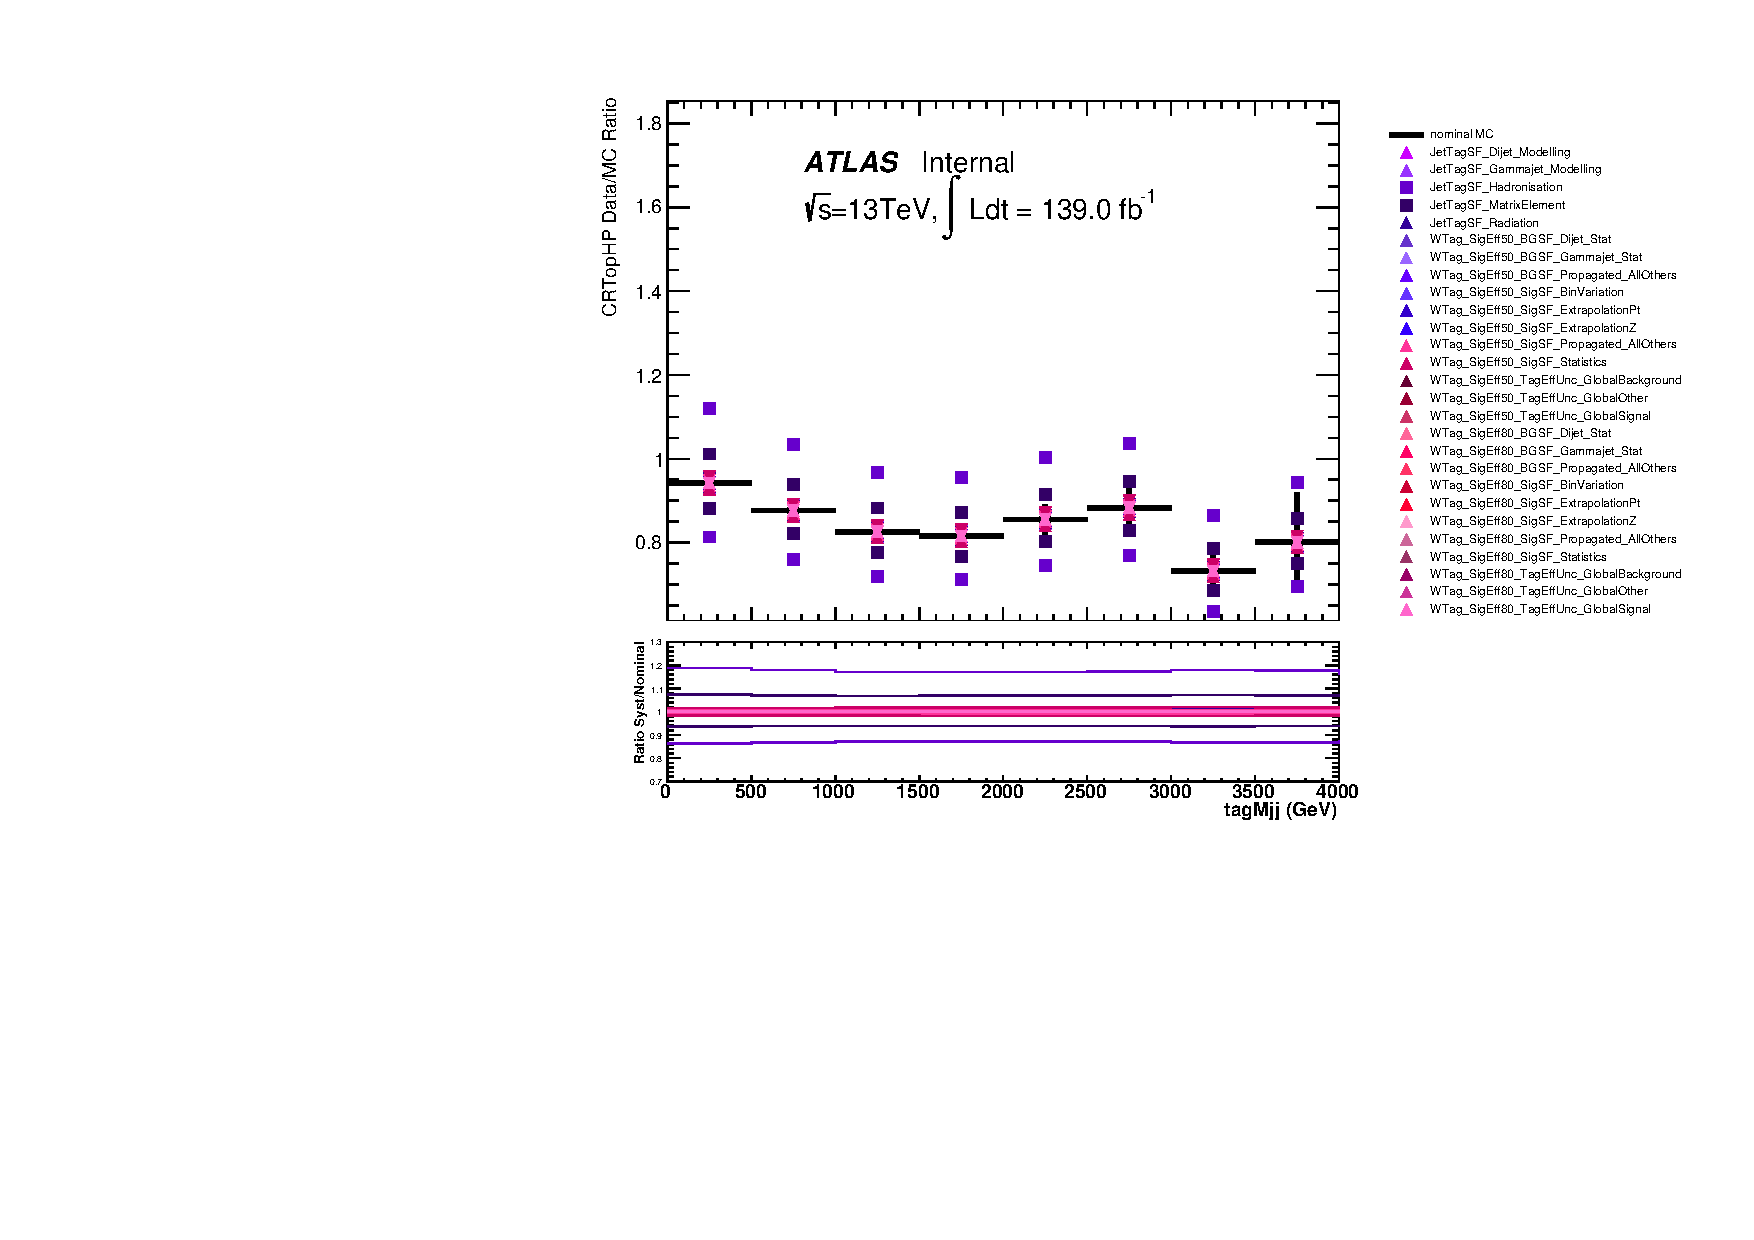
\includegraphics[width=\textwidth]{figures/1lep/VTaggerUnc/VTagCRTopHPtagMjj_SystBreakDown.pdf}
        \caption{Merged HP TopCR}
        \label{fig:MergedHPTopCR}
    \end{subfigure}
%    \hfill % This adds a bit of horizontal spacing between figures
    \begin{subfigure}[b]{0.3\textwidth}
        \centering
        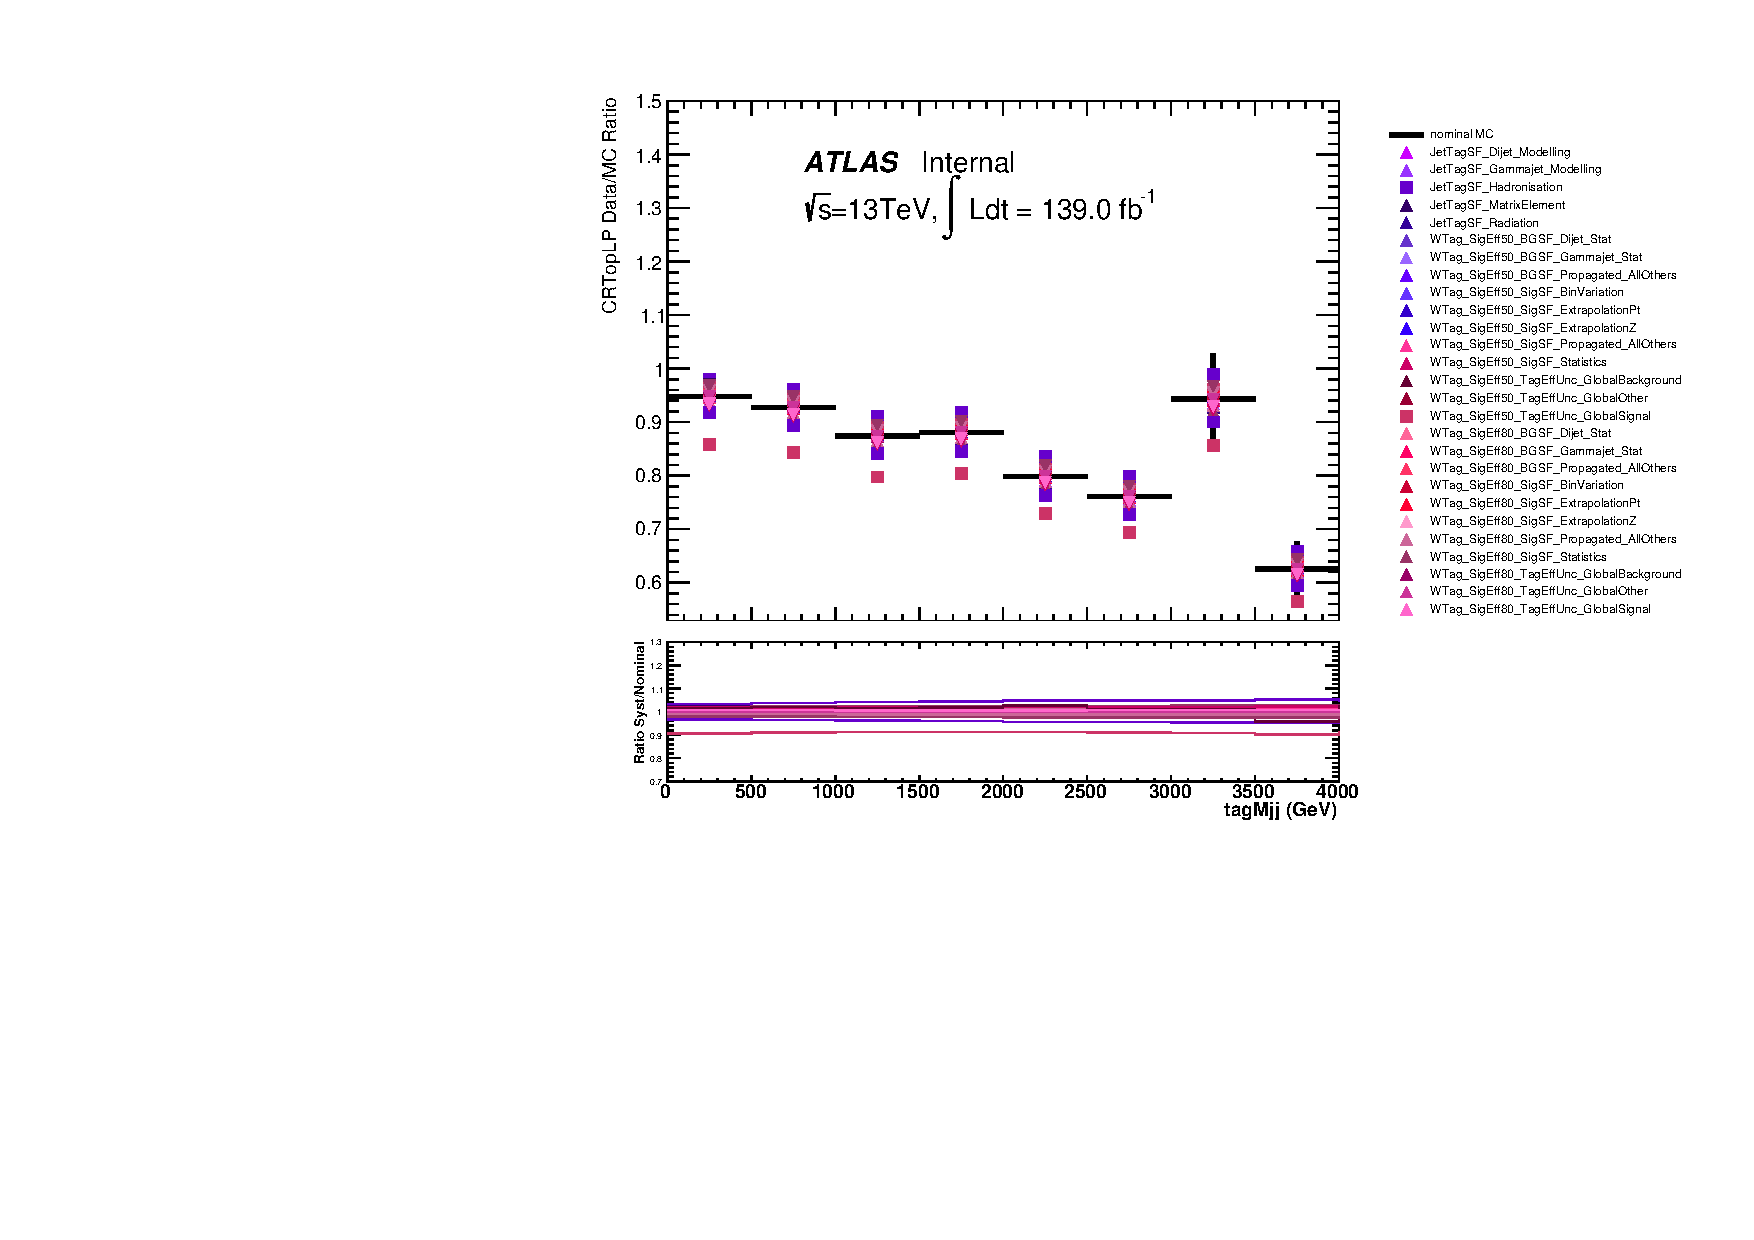
\includegraphics[width=\textwidth]{figures/1lep/VTaggerUnc/VTagCRTopLPtagMjj_SystBreakDown.pdf}
        \caption{Merged LP TopCR}
        \label{fig:MergedLPTopCR}
    \end{subfigure}
%    \hfill % This adds a bit of horizontal spacing between figures
    \begin{subfigure}[b]{0.3\textwidth}
        \centering
        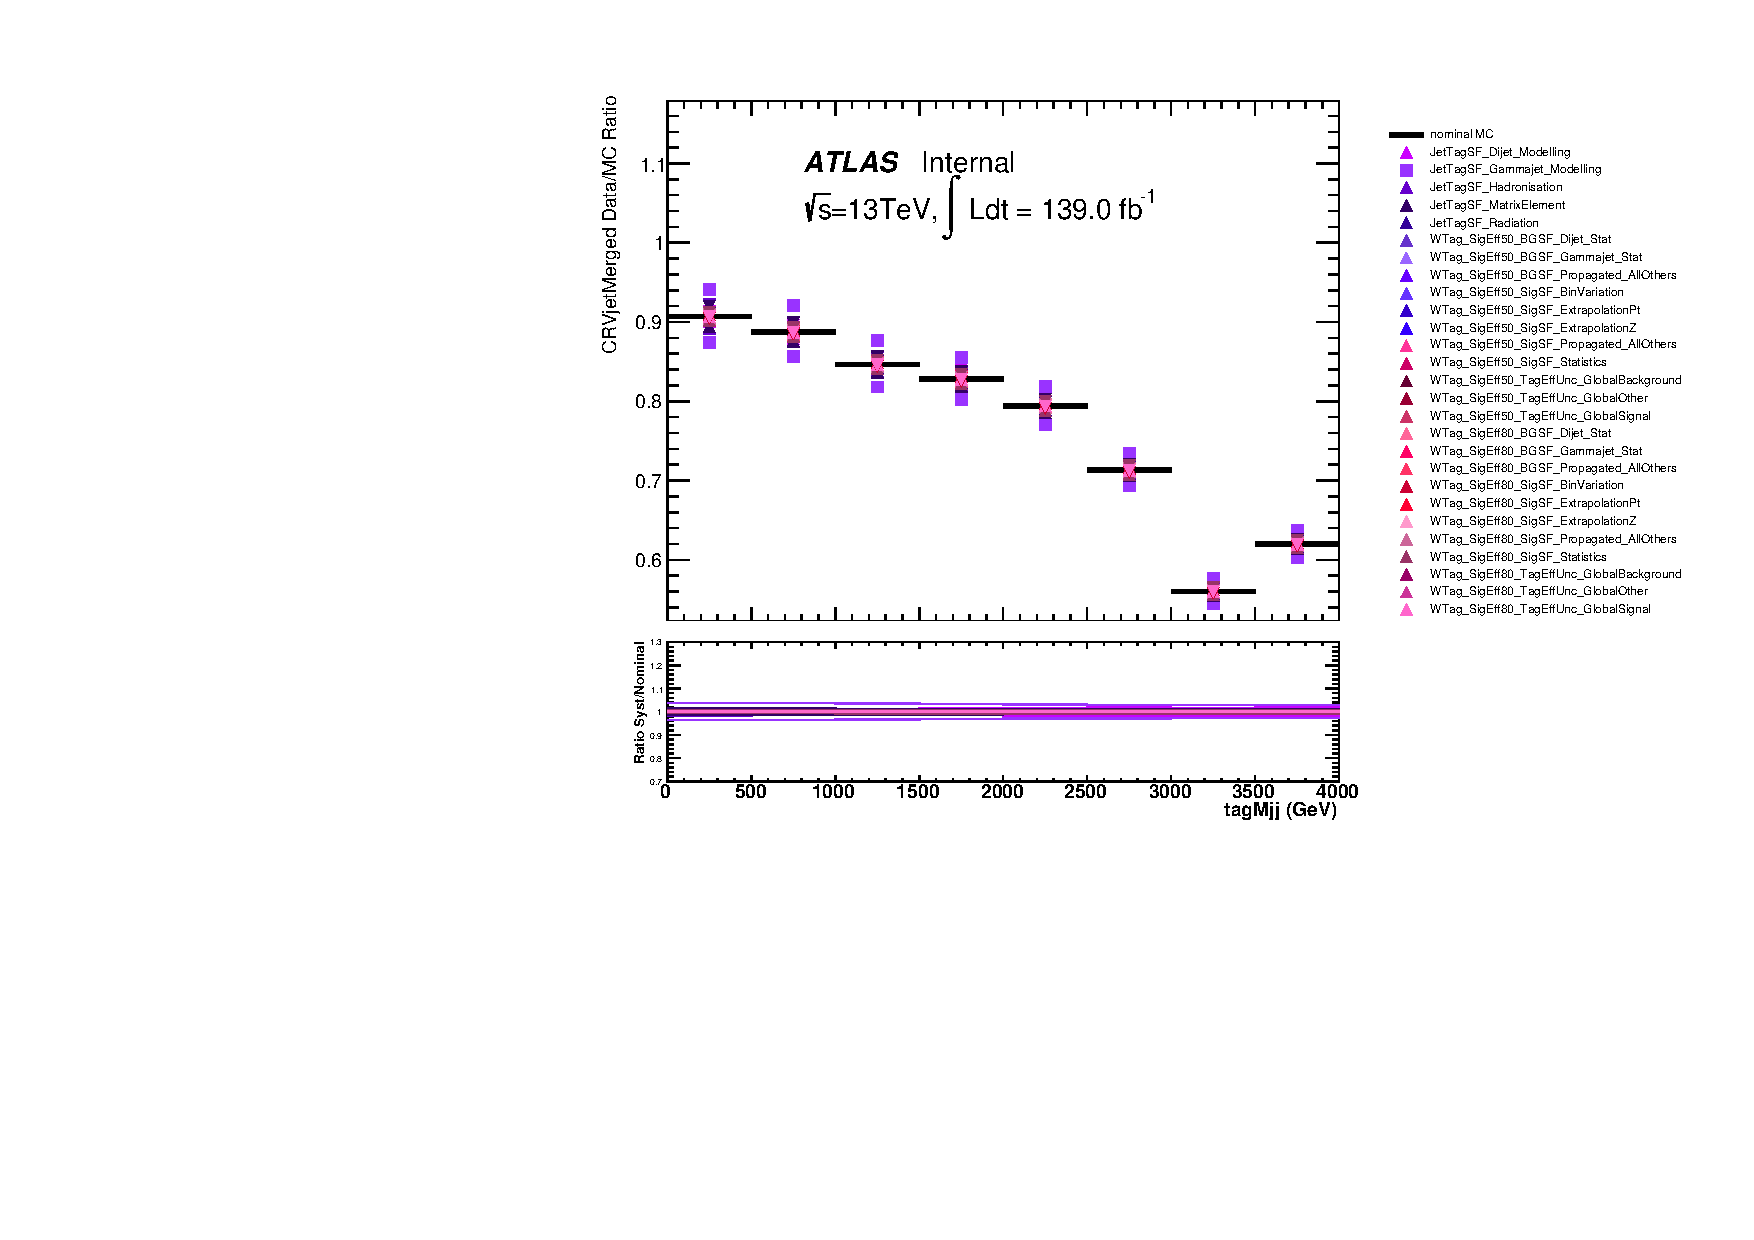
\includegraphics[width=\textwidth]{figures/1lep/VTaggerUnc/VTagCRVjetMergedtagMjj_SystBreakDown.pdf}
        \caption{Merged Wjets CR}
        \label{fig:MergedWjetsCR}
    \end{subfigure}
    \caption{Comparison of boson tagging scale factors in the 1-lepton channel.}
    \label{fig:1LepVTaggerUnc}
\end{figure}


%%%\begin{figure}[ht]
%%%    \centering
%%%        \subfigure[Merged CR]{\includegraphics[width=0.3\textwidth]{figures/2lep/taggerSF/0_MTagMerJets_SYS_CRVjet.pdf}}
%%%    	\subfigure[Merged HP SR]{\includegraphics[width=0.3\textwidth]{figures/2lep/taggerSF/0_MTagMerJets_SYS_SRVBS_HP.pdf}}
%%%        \subfigure[Merged LP SR]{\includegraphics[width=0.3\textwidth]{figures/2lep/taggerSF/0_MTagMerJets_SYS_SRVBS_LP.pdf}}
%%%        \caption{ Data/MC ratios as a function of the mass of the tagging jets in the 2-lepton channel. All tagger SF related uncertainties are plotted. The plots are before applying the re-weighting described in \ref{subsec:mjj_reweight_2lep}. All bins containing more than 5\% of signal are blinded in the SRs. } 
%%%    \label{fig:2lep_bkgUnc_BT}
%%%\end{figure}


%%%\begin{figure}[ht]
%%%    \centering
%%%        \subfigure[Merged HP TopCR]{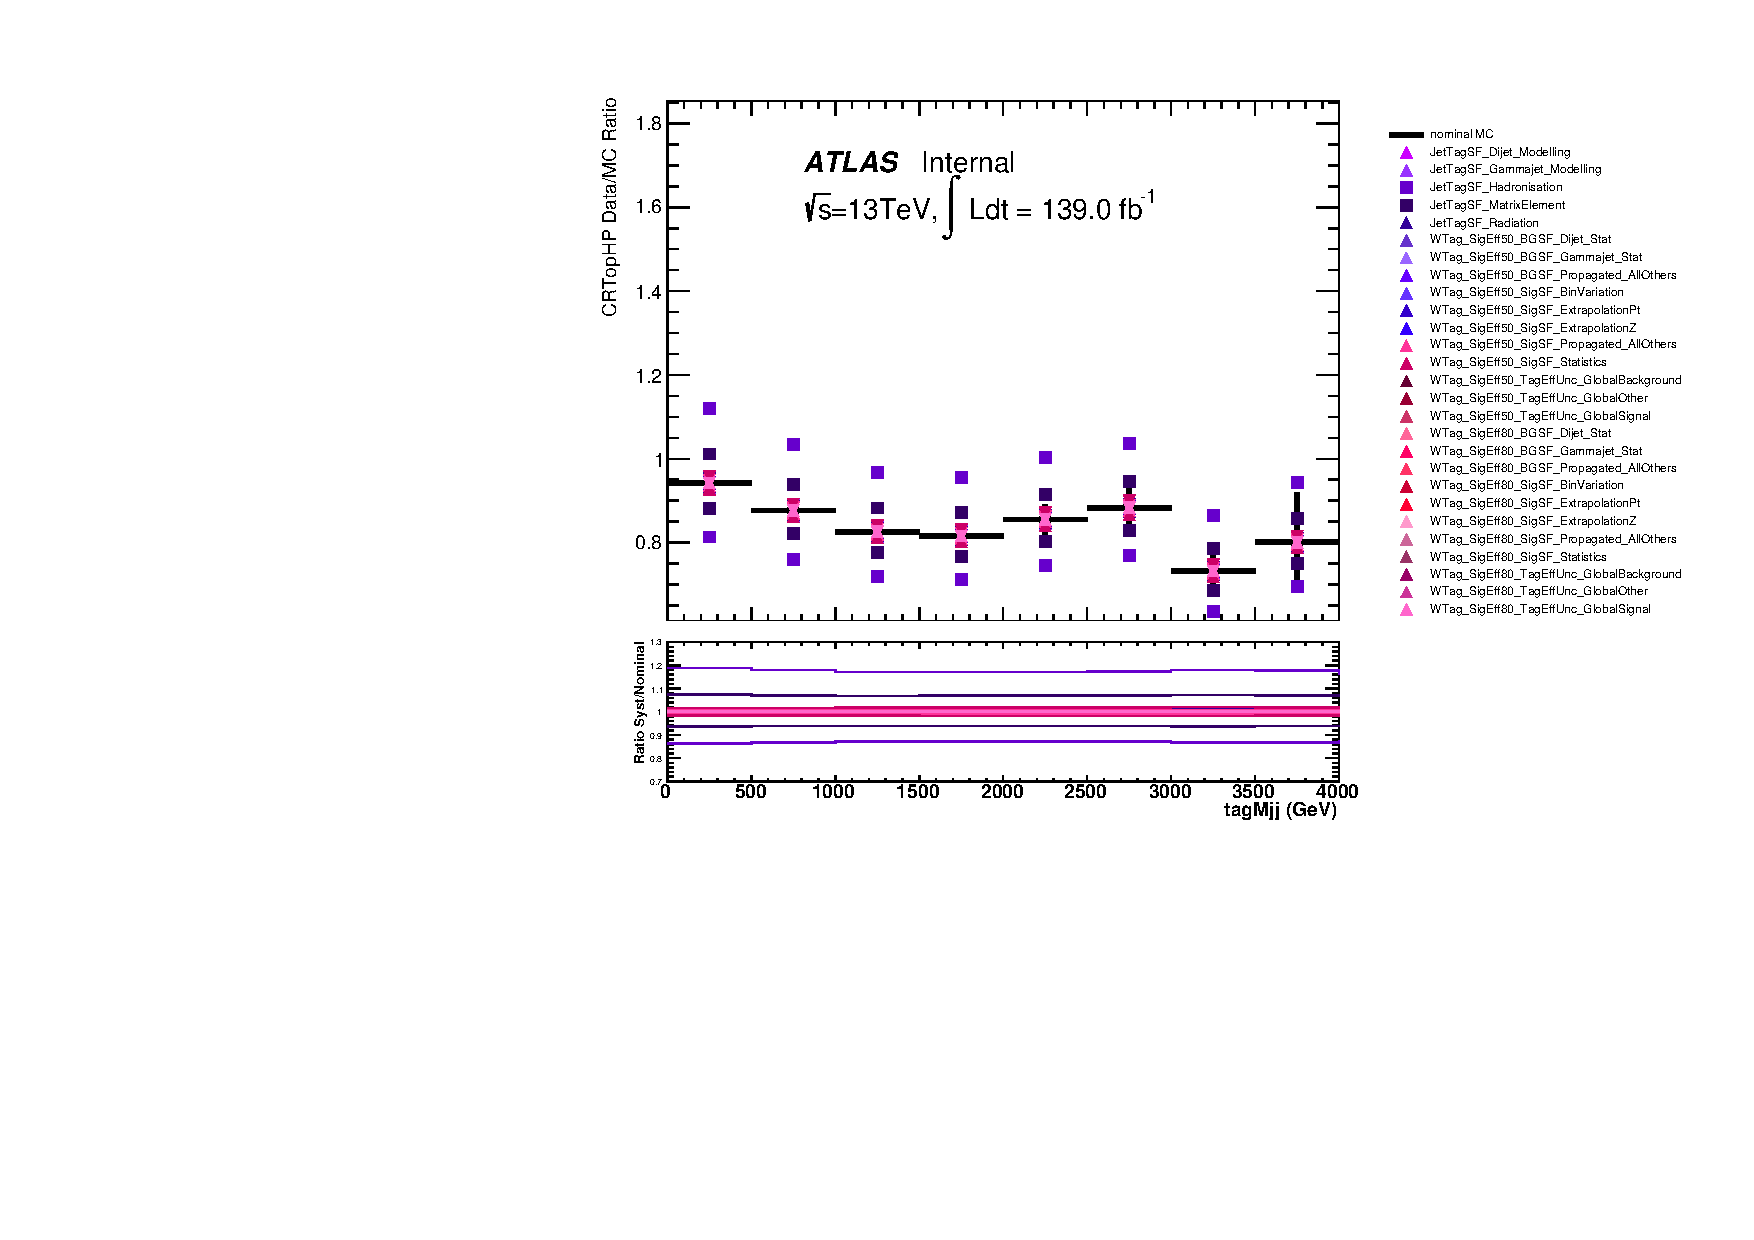
\includegraphics[width=0.3\textwidth]{figures/1lep/VTaggerUnc/VTagCRTopHPtagMjj_SystBreakDown.pdf}}
%%%    	\subfigure[Merged LP TopCR]{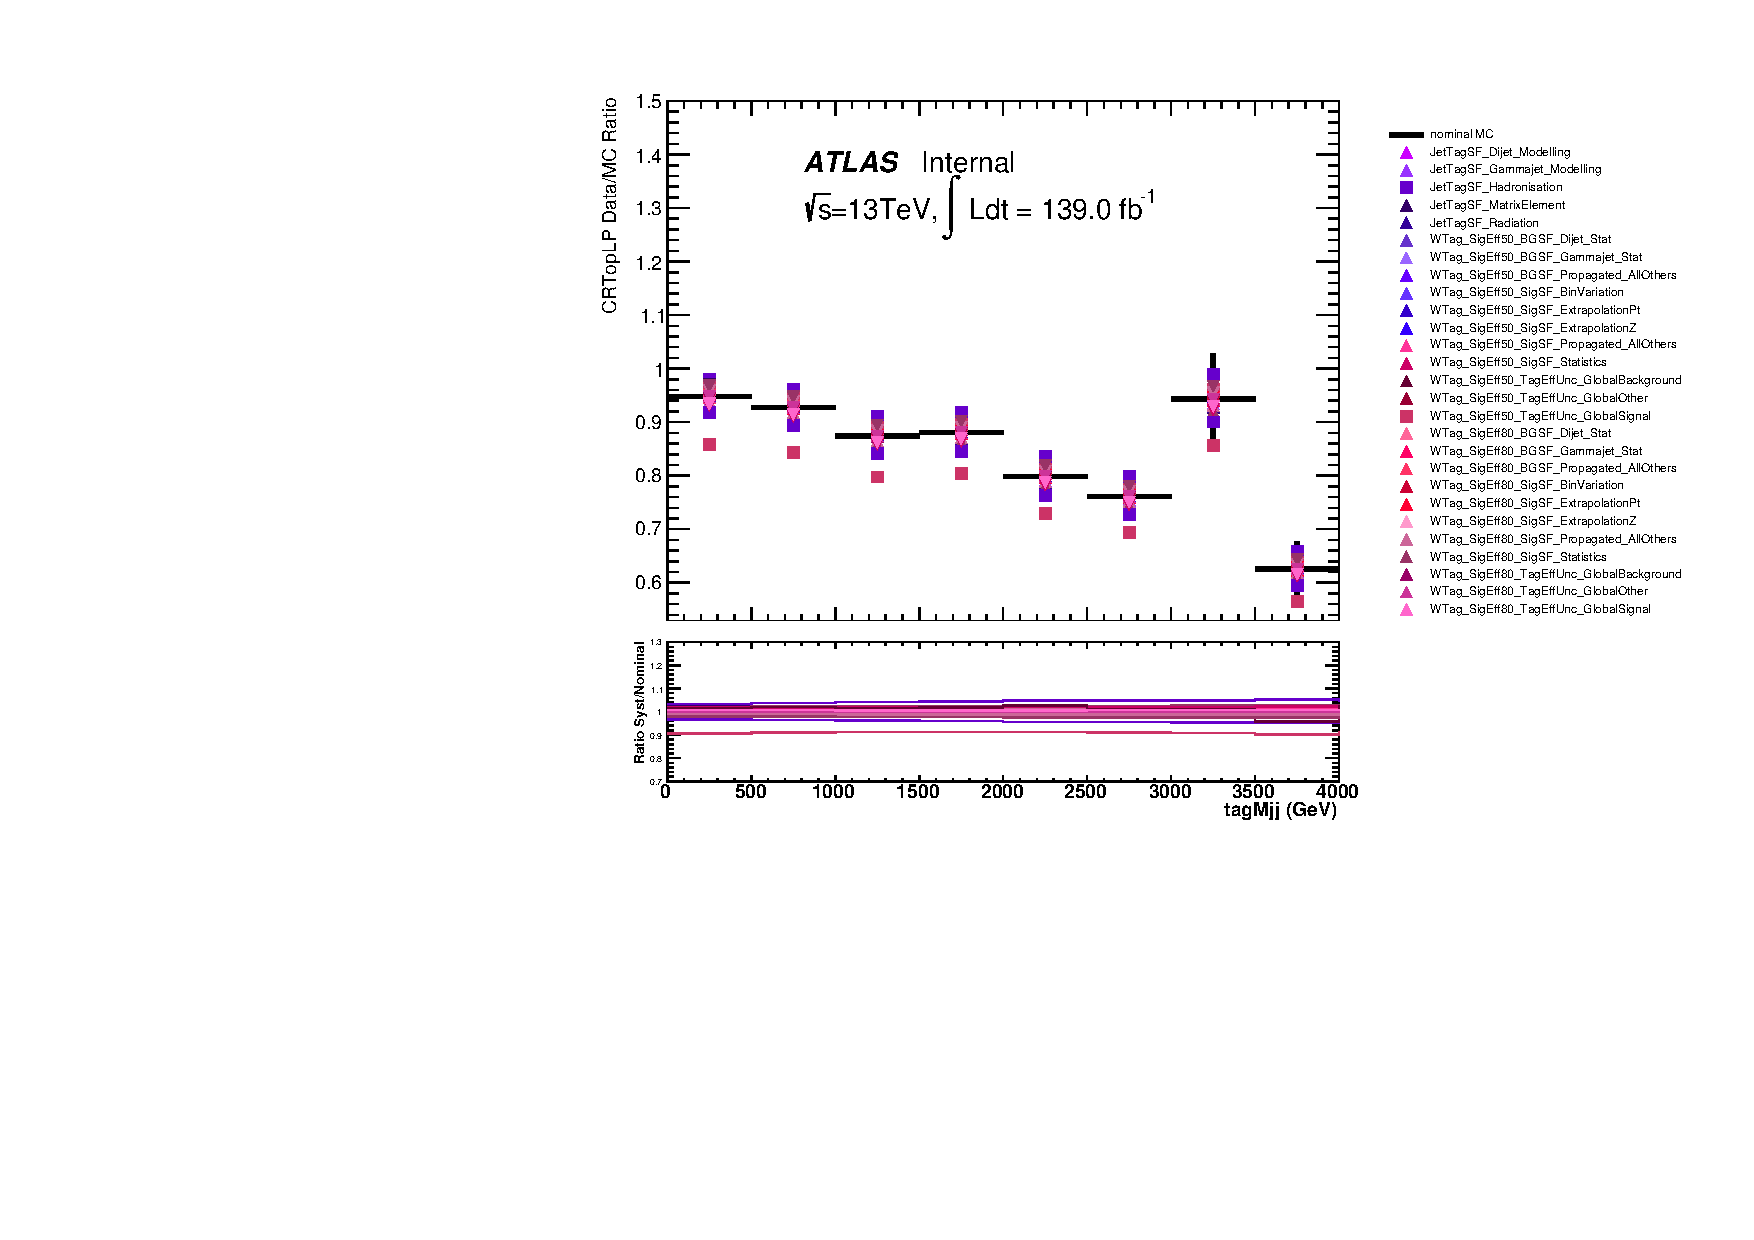
\includegraphics[width=0.3\textwidth]{figures/1lep/VTaggerUnc/VTagCRTopLPtagMjj_SystBreakDown.pdf}} 
%%%	\subfigure[Merged Wjets CR]{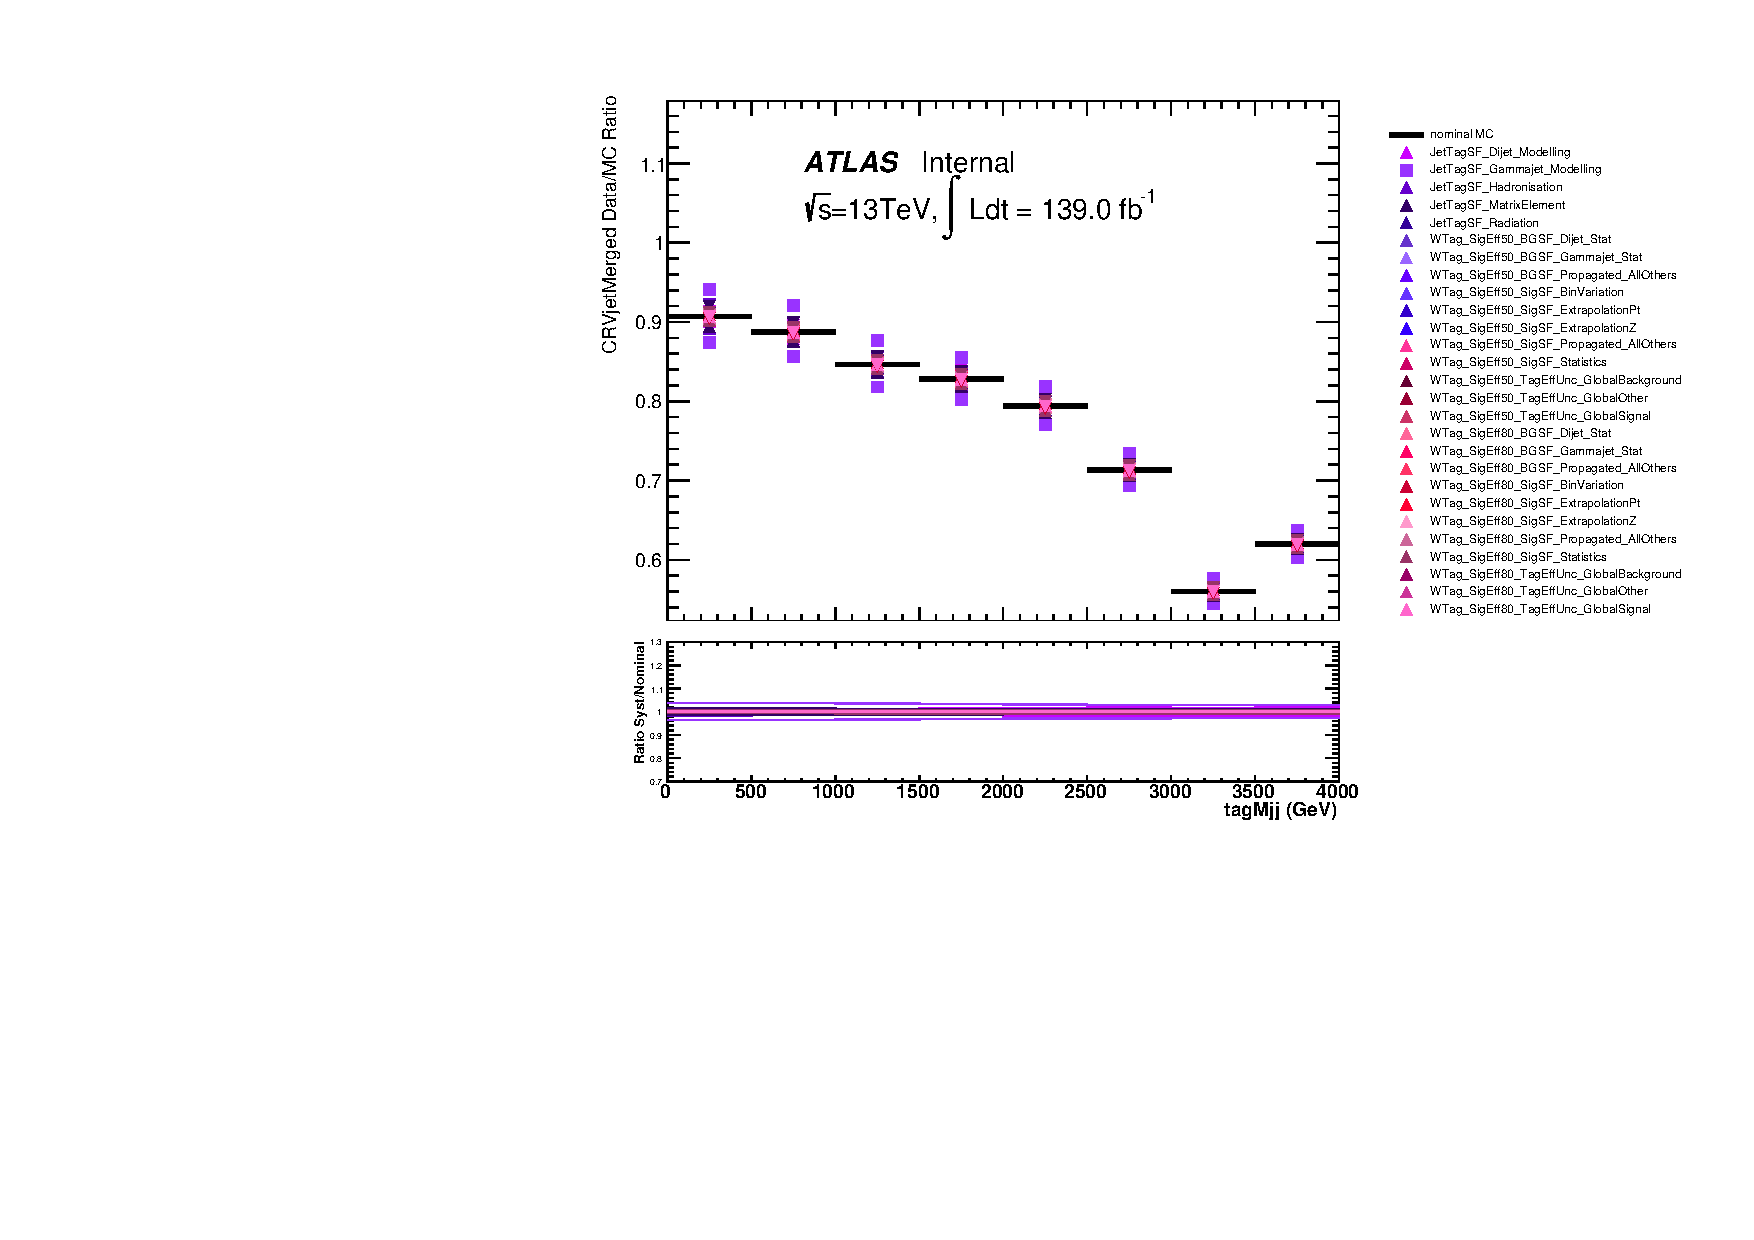
\includegraphics[width=0.3\textwidth]{figures/1lep/VTaggerUnc/VTagCRVjetMergedtagMjj_SystBreakDown.pdf}}
%%%        \caption{Comparison of boson tagging scale factors in the 1-lepton channel. } 
%%%    \label{fig:1LepVTaggerUnc}
%%%\end{figure}


%%%\begin{figure}[ht]
%%%    \centering
%%%      	\subfigure[signal: Merged CR]{\includegraphics[width=0.3\textwidth]{figures/0lep/systematics/systs/merged/plots/systvtagSigsig_RNN_CRVjet_Mer.pdf}}
%%%    	\subfigure[signal: Merged HP SR]{\includegraphics[width=0.3\textwidth]{figures/0lep/systematics/systs/merged/plots/systvtagSigsig_RNN_SRVBS_HP.pdf}}
%%%        \subfigure[signal: Merged LP SR]{\includegraphics[width=0.3\textwidth]{figures/0lep/systematics/systs/merged/plots/systvtagSigsig_RNN_SRVBS_LP.pdf}}\\
%%%      	\subfigure[background: Merged CR]{\includegraphics[width=0.3\textwidth]{figures/0lep/systematics/systs/merged/plots/systvtagBkgWjets_nom_Zjets_nom_diboson_stop_ttbar_nom_RNN_CRVjet_Mer.pdf}}
%%%    	\subfigure[background: Merged HP SR]{\includegraphics[width=0.3\textwidth]{figures/0lep/systematics/systs/merged/plots/systvtagBkgWjets_nom_Zjets_nom_diboson_stop_ttbar_nom_RNN_SRVBS_HP.pdf}}
%%%        \subfigure[background: Merged LP SR]{\includegraphics[width=0.3\textwidth]{figures/0lep/systematics/systs/merged/plots/systvtagBkgWjets_nom_Zjets_nom_diboson_stop_ttbar_nom_RNN_SRVBS_HP.pdf}}\\
%%%        \caption{Effect of all tagger SF related uncertainties in the 0-lepton channel on the signal MC and on all background MCs together.} 
%%%    \label{fig:0LepVTaggerUnc}
%%%\end{figure}



%%%
\subsection{Quark/Gluon jets uncertainty}
%\subsubsection{Quark/Gluon jets uncertainty}
\label{subsec:bkg_uncer_qg}

Jet flavor response and composition uncertainties consider the different jet responses to quark- and gluon-initiated jets. 
The response uncertainties are centrally derived from dijet events using alternative MC samples, specifically Pythia 8 and Herwig++. 
For flavor composition, uncertainties are typically assumed based on a 50/50 quark/gluon mix, with a conservative (100\%) uncertainty. 
However, in VBS topologies, which tend to be quark-enriched, such uncertainties can limit measurement sensitivity. 
To mitigate this, we study the gluon fraction within our analysis phase-space. 
This allows us to rederive jet flavor-related uncertainties using custom gluon fractions, thus potentially reducing these uncertainties.

The estimation of the gluon fraction across various analysis regions and samples is performed as a function of the small-\(R\) jet \(\pt\) and \(\eta\). This is achieved by utilizing truth parton label information to discern the quantity of quarks and gluons. For the purpose of quark estimation, all jets are considered in the denominator, with the exception of those initiated by b-quarks.

The gluon fraction for each analysis region and across various samples is calculated based on the small-$R$ jet $\pt$ and $\eta$. 
This estimation utilizes truth parton label information to determine the number of quarks and gluons. 
For the purpose of quark estimation, all jets except those initiated by $b$-quarks are considered in the denominator.

Two-dimensional histograms, representing the gluon fraction as a function of jet $\pt$ and $\eta$, serve as inputs for recalculating jet flavor and composition uncertainties. Each MC sample is associated with a single input file. 
The gluon fraction for a specific ($\pt$, $\eta$) bin is determined by aggregating data across all regions, according to the nominal approach.

To account for the uncertainty in the gluon fraction, additional inputs are utilized. The uncertainty for a particular ($\pt$, $\eta$) bin, $\sigma_{gfrac}$, is calculated as follows:
\[
\sigma_{gfrac} = \sqrt{\sigma_{region}^{2} + \sigma_{gen}^{2}}
\]
Here, \(\sigma_{region}\) represents the maximal deviation in gluon fraction between the nominal and any analysis region. Meanwhile, \(\sigma_{gen}\) denotes the generator uncertainty, obtained from comparing alternative Pythia 8 and Herwig++ MC samples.


The inputs for the gluon fraction and their corresponding uncertainties in the \olep channel are illustrated in Figures \ref{fig:QGFracInputs2D1Lep} and \ref{fig:QGFracErrorInputs2D1Lep}, respectively. 
Comparison between old flavor uncertainties and newly derived flavor uncertainties is shown is Figure \ref{fig:1LepFlavorVarOldNew}. It is evident from this comparison that flavor composition uncertainties, in general, are reduced.


%%%%%%%%
%%%The jet flavor response and composition uncertainties account for the different jet responses to quark- and gluon-initiated jets. The flavor response uncertainties are derived centrally from dijet events using alternative (Pythia 8 and Herwig++) Monte Carlo. Flavor composition uncertainties are usually derived assuming a 50/50 quark/gluon composition with a very conservative (100\%) uncertainty. In VBS topologies where quark enriched regions are expected such uncertainties can limit the sensitivity of the measurement. In order to reduce such uncertainties, the gluon fraction in our analysis phase-space is studied and jet flavor related uncertainties are rederived using custom gluon fractions. %anastasia; Maybe add formulas for jet flavour composition and jet flavour response from dimitris lectures
%%%
%%%The gluon fraction in each of the analysis regions and for the different analysis samples is estimated as a function of the small-$R$ jet $\pt$ and $\eta$. Truth parton label information is used in order to estimate the number of quarks and gluons.  All jets except b-quark-initiated jets are included in the denominator for the quark estimation. 
%%%
%%%In Figures \ref{fig:2lep_gfrac_pt} and  \ref{fig:2lep_gfrac_eta} a comparison of the gluon fraction between the different analysis regions for the 2-lepton channel main MC samples is plotted as a function of $\pt$ and $\eta$ respectively. A clear $\pt$ and $\eta$ dependence of the gluon fraction is noticed.
%%%
%%%2D histograms of the gluon fraction as a function of  $\pt$ and $\eta$ are used as inputs to recalculate the jet flavor and composition uncertainties. A single input file per MC sample is used. The gluon fraction for a given bin in $\pt$ and $\eta$ is given after summing up all regions (nominal approach). This approach is very similar to computing the average gluon fraction between regions as shown by comparing the red and black histograms of Figure \ref{fig:2lep_gfrac_eta}. Additional inputs to describe the uncertainty on the gluon fraction are also provided. The uncertainty in a given $\pt,\eta$ bin is given by: $$ \sigma_{gfrac} = \sqrt{\sigma_{region}^{2}+\sigma_{gen}^{2} } $$ where $\sigma_{region}$ is the maximum difference in gluon fraction between nominal and an analysis region, $\sigma_{gen}$ is the generator uncertainty derived using alternative Pythia 8 and Herwig MC samples. In Figures \ref{fig:2lep_gfrac_alt_pt} and  \ref{fig:2lep_gfrac_alt_eta} a comparison of the nominal gluon fraction and gluon fraction as calculated by using alternative samples is plotted for the main background sources in the 2-lepton channel. For cases where alternative samples are not available (e.g for Signal) the region only uncertainties are considered. %anastasia; maybe comment that the region uncertainties are usually much larger than the ones coming from alternative samples.
%%%
%%%The gluon fraction inputs and their corresponding uncertainties for the 2-lepton channel are plotted in Figures  \ref{fig:2lep_gfrac_2D} and  \ref{fig:2lep_gfrac_err_2D} respectively. Similar plots for the 0- and 1-lepton channels can be found in appendix \ref{app:QGfraction}. 

%%%%%%%%%%%%%


\begin{figure}[p]
    \centering
    \begin{subfigure}[b]{0.3\textwidth}
        \centering
        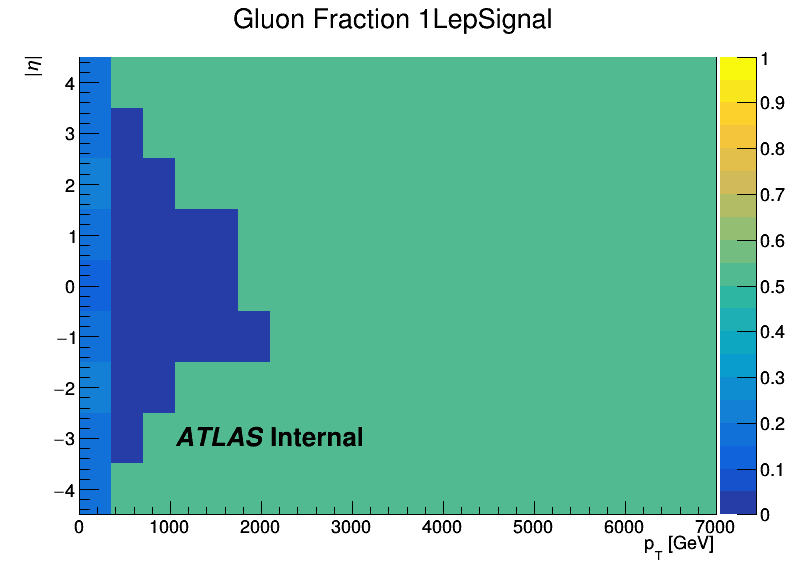
\includegraphics[width=\textwidth]{figures/QGfrac/GluonFrac2D_1LepSignal.png}
        \caption{Signal samples}
        \label{fig:GluonFracSignal}
    \end{subfigure}
    \hfill
    \begin{subfigure}[b]{0.3\textwidth}
        \centering
        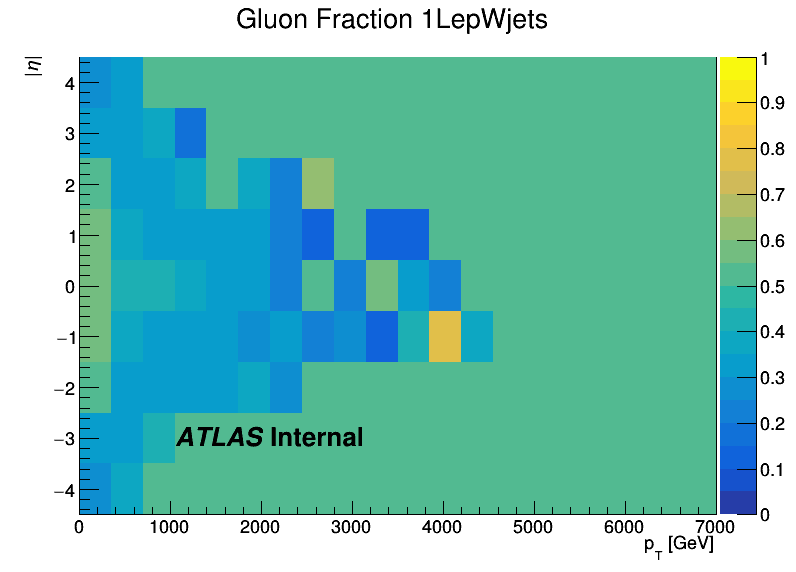
\includegraphics[width=\textwidth]{figures/QGfrac/GluonFrac2D_1LepWjets.png}
        \caption{\Wjets samples}
        \label{fig:GluonFracWjets}
    \end{subfigure}
    \hfill
    \begin{subfigure}[b]{0.3\textwidth}
        \centering
        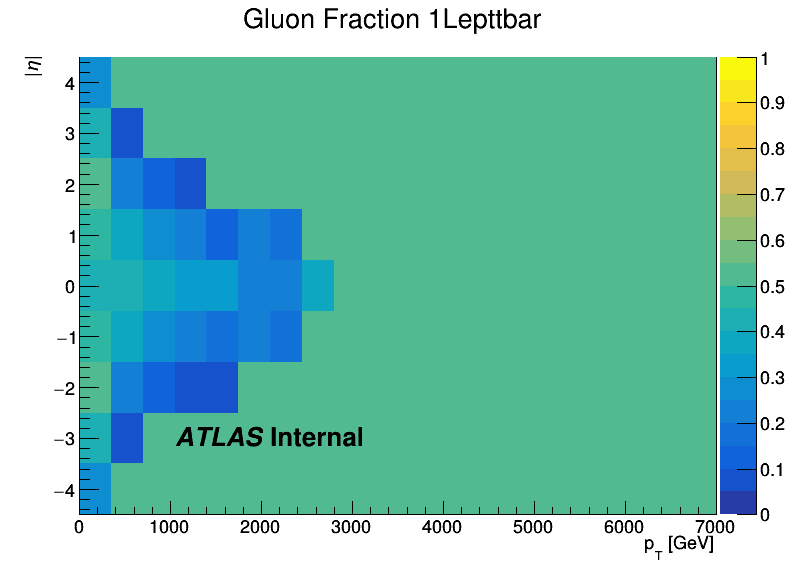
\includegraphics[width=\textwidth]{figures/QGfrac/GluonFrac2D_1Lepttbar.png}
        \caption{ttbar samples}
        \label{fig:GluonFracttbar}
    \end{subfigure}

    \bigskip

    \begin{subfigure}[b]{0.3\textwidth}
        \centering
        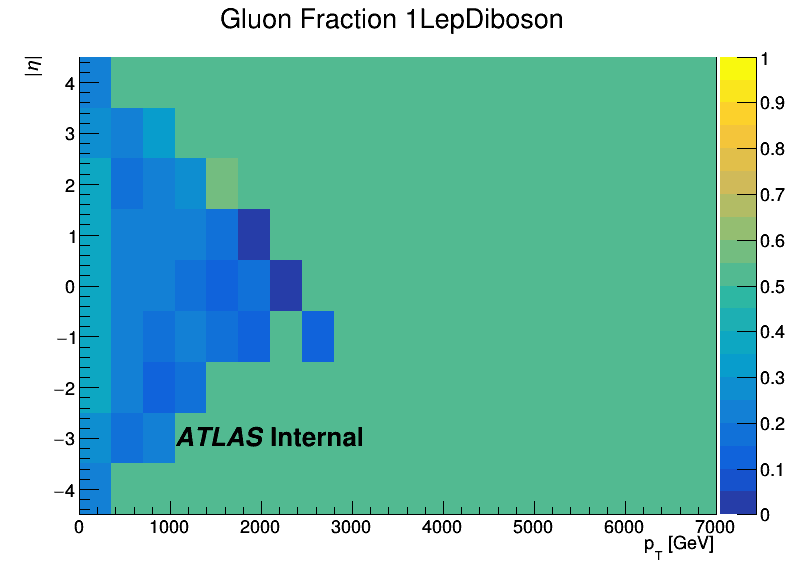
\includegraphics[width=\textwidth]{figures/QGfrac/GluonFrac2D_1LepDiboson.png}
        \caption{Diboson samples}
        \label{fig:GluonFracDiboson}
    \end{subfigure}
%    \hfill
    \begin{subfigure}[b]{0.3\textwidth}
        \centering
        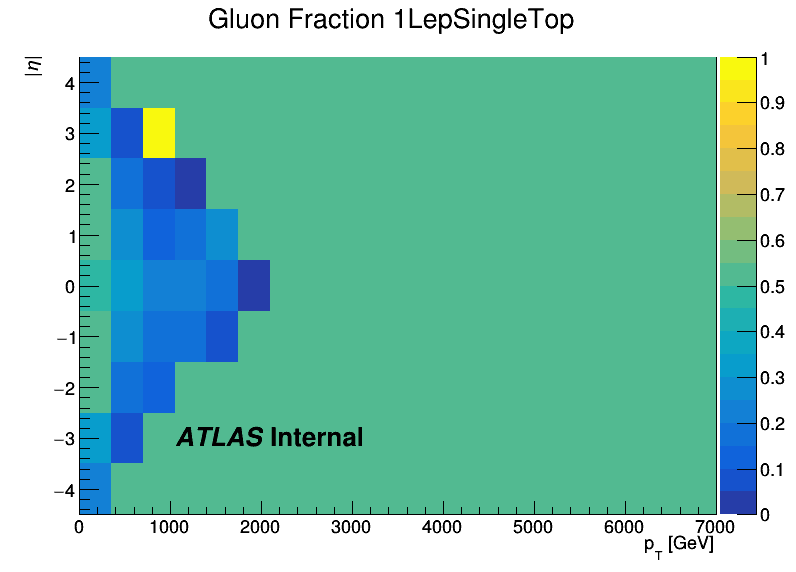
\includegraphics[width=\textwidth]{figures/QGfrac/GluonFrac2D_1LepSingleTop.png}
        \caption{Single top samples}
        \label{fig:GluonFracSingleTop}
    \end{subfigure}
    \hfill

    \caption{Gluon fraction inputs used to calculate jet uncertainties for the 1 lepton channel.}
    \label{fig:QGFracInputs2D1Lep}
\end{figure}


\begin{figure}[p]
    \centering
    \begin{subfigure}[b]{0.3\textwidth}
        \centering
        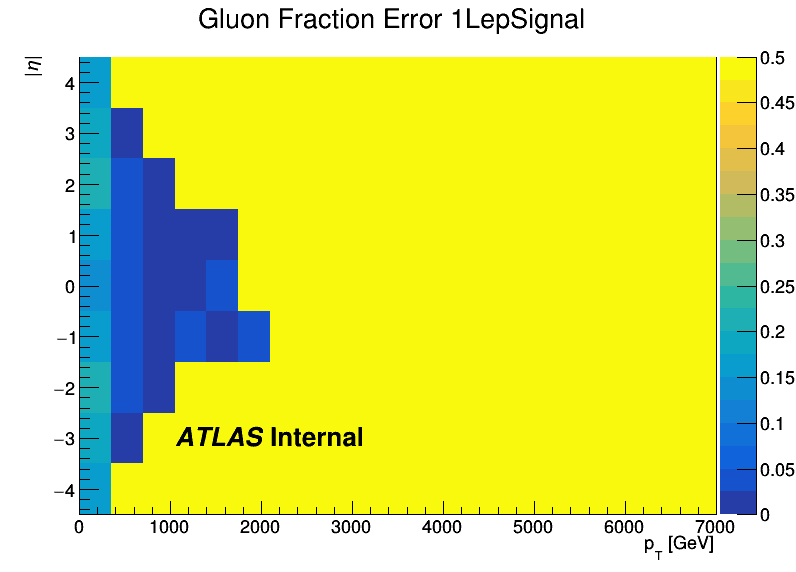
\includegraphics[width=\textwidth]{figures/QGfrac/GluonFracError2D_1LepSignal.png}
        \caption{Signal samples}
        \label{fig:GluonFracErrorSignal}
    \end{subfigure}
    \hfill
    \begin{subfigure}[b]{0.3\textwidth}
        \centering
        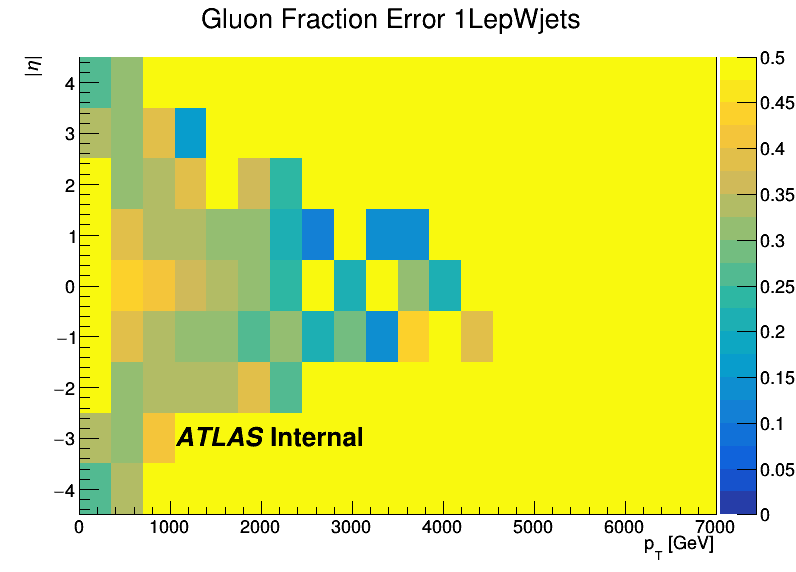
\includegraphics[width=\textwidth]{figures/QGfrac/GluonFracError2D_1LepWjets.png}
        \caption{\Wjets samples}
        \label{fig:GluonFracErrorWjets}
    \end{subfigure}
    \hfill
    \begin{subfigure}[b]{0.3\textwidth}
        \centering
        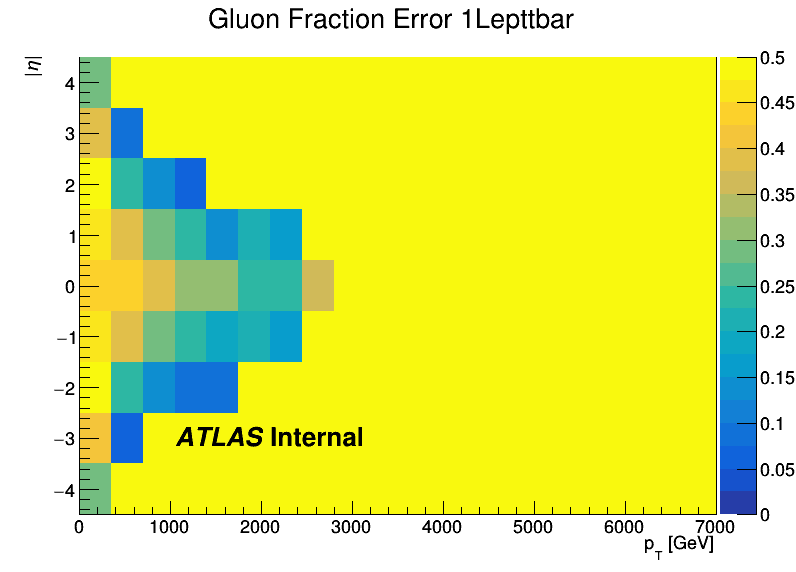
\includegraphics[width=\textwidth]{figures/QGfrac/GluonFracError2D_1Lepttbar.png}
        \caption{ttbar samples}
        \label{fig:GluonFracErrorttbar}
    \end{subfigure}

    \bigskip

    \begin{subfigure}[b]{0.3\textwidth}
        \centering
        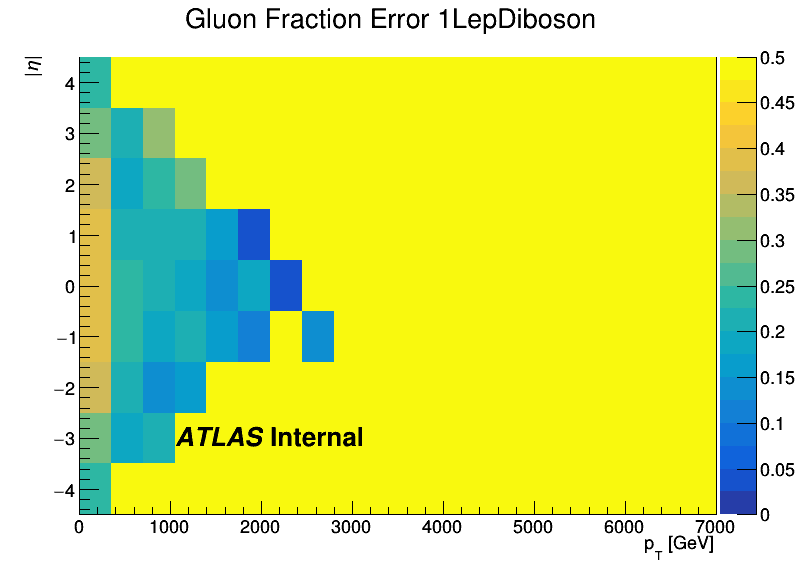
\includegraphics[width=\textwidth]{figures/QGfrac/GluonFracError2D_1LepDiboson.png}
        \caption{Diboson samples}
        \label{fig:GluonFracErrorDiboson}
    \end{subfigure}
%    \hfill
    \begin{subfigure}[b]{0.3\textwidth}
        \centering
        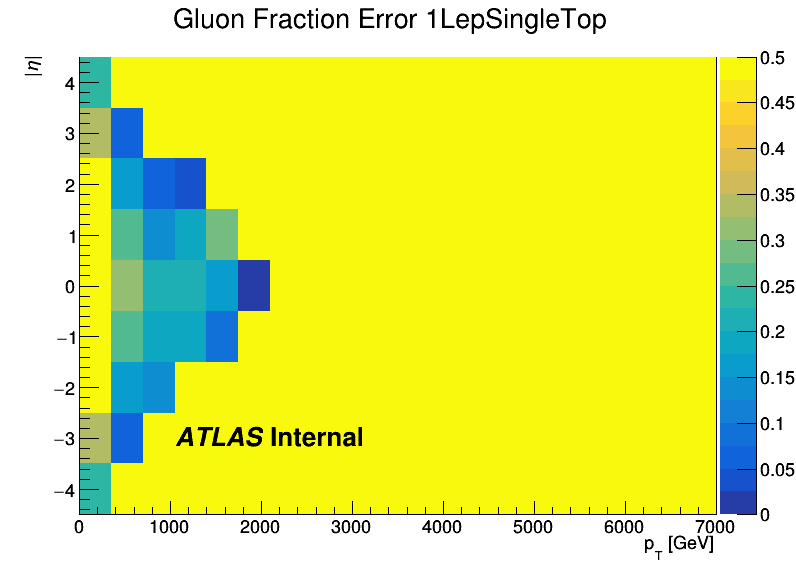
\includegraphics[width=\textwidth]{figures/QGfrac/GluonFracError2D_1LepSingleTop.png}
        \caption{Single top samples}
        \label{fig:GluonFracErrorSingleTop}
    \end{subfigure}
    \hfill

    \caption{Gluon fraction error inputs used to calculate jet uncertainties for the 1 lepton channel.}
    \label{fig:QGFracErrorInputs2D1Lep}
\end{figure}


\begin{figure}[ht]
    \centering
    \begin{subfigure}[b]{0.4\textwidth}
        \centering
        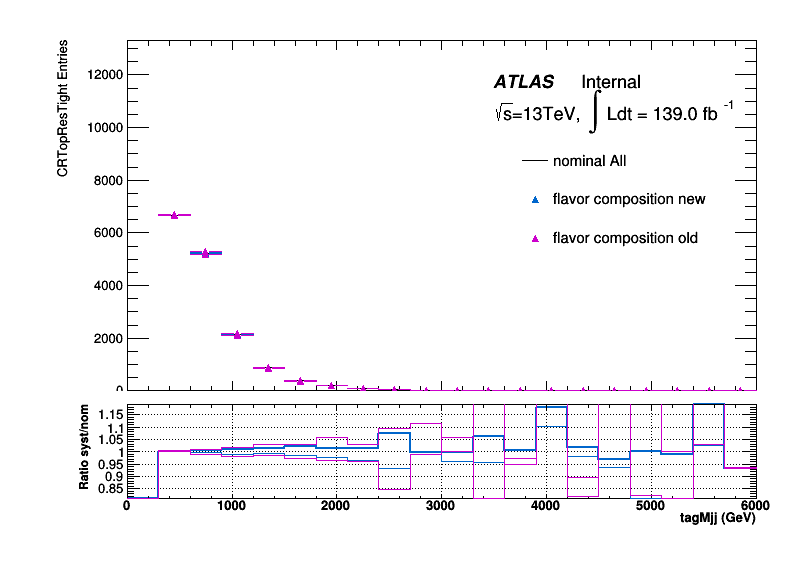
\includegraphics[width=\textwidth]{figures/1lep/FlavorVar/SystFCompCRTopResTight_All_tagMjj.png}
        \caption{Resolved TopCR Flavour Composition}
        \label{fig:ResolvedTopCRFlavourComposition}
    \end{subfigure}
    \quad % This adds some spacing between the figures in the same row
    \begin{subfigure}[b]{0.4\textwidth}
        \centering
        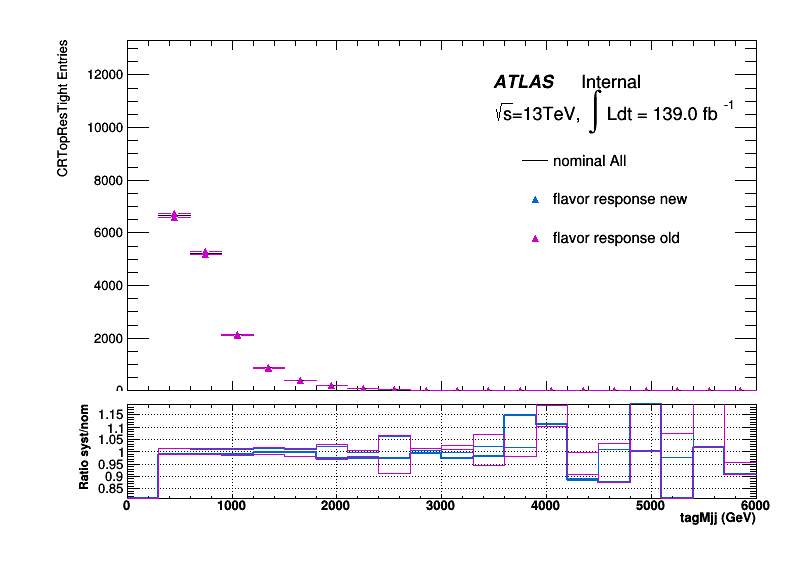
\includegraphics[width=\textwidth]{figures/1lep/FlavorVar/SystFResCRTopResTight_All_tagMjj.png}
        \caption{Resolved TopCR Flavour Response}
        \label{fig:ResolvedTopCRFlavourResponse}
    \end{subfigure}

    \bigskip % This adds extra vertical spacing between the rows of figures

    \begin{subfigure}[b]{0.4\textwidth}
        \centering
        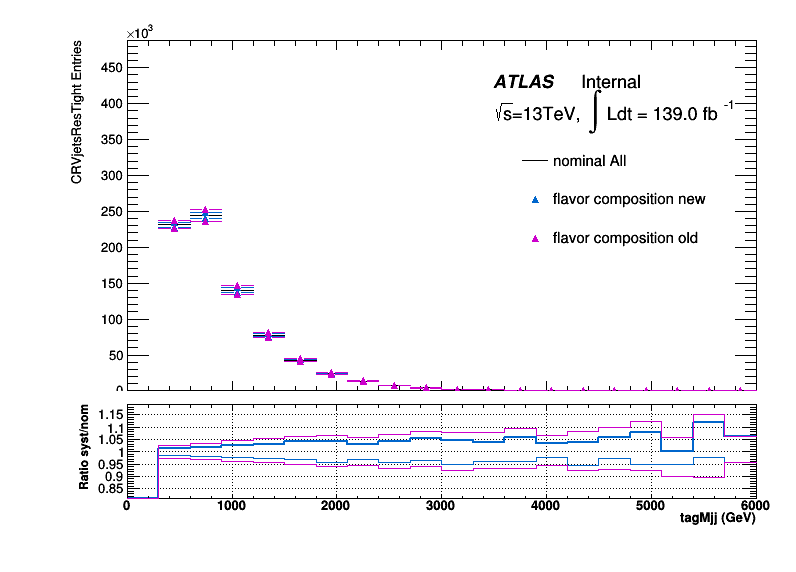
\includegraphics[width=\textwidth]{figures/1lep/FlavorVar/SystFCompCRVjetsResTight_All_tagMjj.png}
        \caption{Resolved WjetsCR Flavour Composition}
        \label{fig:ResolvedWjetsCRFlavourComposition}
    \end{subfigure}
    \quad % This adds some spacing between the figures in the same row
    \begin{subfigure}[b]{0.4\textwidth}
        \centering
        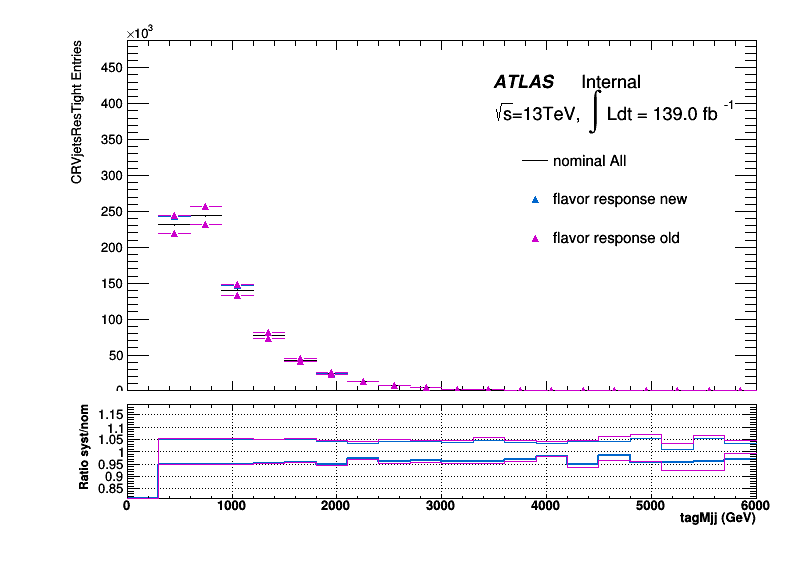
\includegraphics[width=\textwidth]{figures/1lep/FlavorVar/SystFResCRVjetsResTight_All_tagMjj.png}
        \caption{Resolved WjetsCR Flavour Response}
        \label{fig:ResolvedWjetsCRFlavourResponse}
    \end{subfigure}

    \caption{Comparison between old flavor uncertainties and newly derived flavor uncertainties.}
    \label{fig:1LepFlavorVarOldNew}
\end{figure}


% Flavour Variations for mc16a 1lep
%%%\begin{figure}[ht]
%%%    \centering
%%%        \subfigure[Resolved TopCR Flavour Composition]{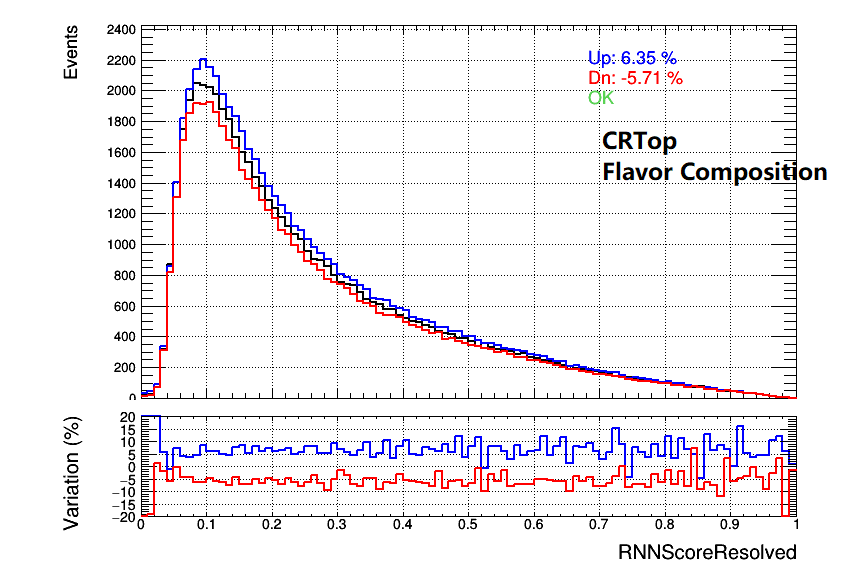
\includegraphics[width=0.4\textwidth]{figures/1lep/FlavorVar/C_0ptag2pjet_0ptv_CRTop_RNNScoreResolved_SysJET_Flavor_Composition.png}}
%%%        \subfigure[Resolved TopCR Flavour Response]{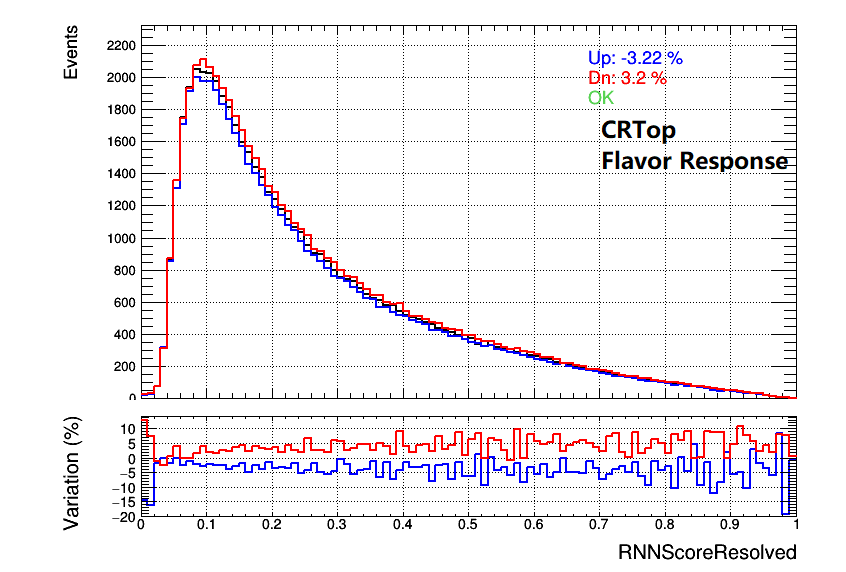
\includegraphics[width=0.4\textwidth]{figures/1lep/FlavorVar/C_0ptag2pjet_0ptv_CRTop_RNNScoreResolved_SysJET_Flavor_Response.png}}\\
%%%
%%%        \subfigure[Resolved WjetCR Flavour Composition]{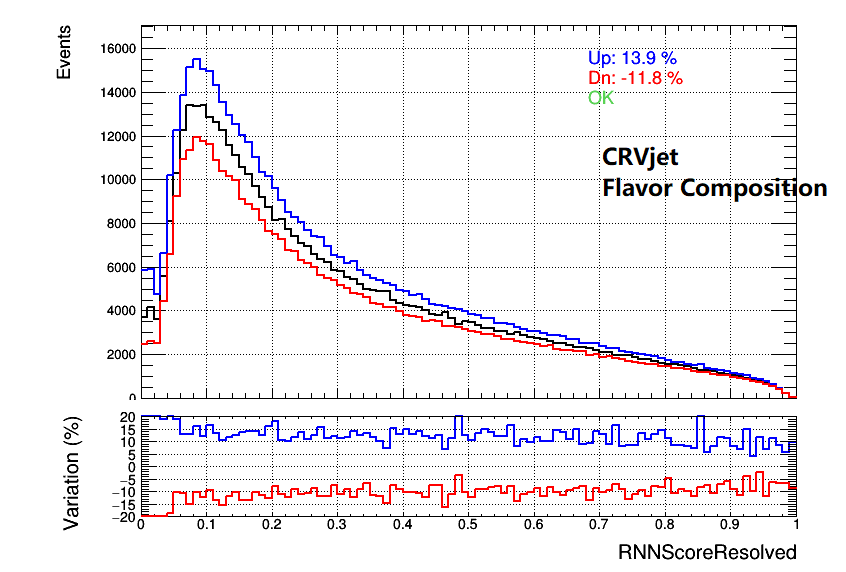
\includegraphics[width=0.4\textwidth]{figures/1lep/FlavorVar/C_0ptag2pjet_0ptv_CRVjet_RNNScoreResolved_SysJET_Flavor_Composition.png}}
%%%	\subfigure[Resolved WjetCR Flavour Reponse]{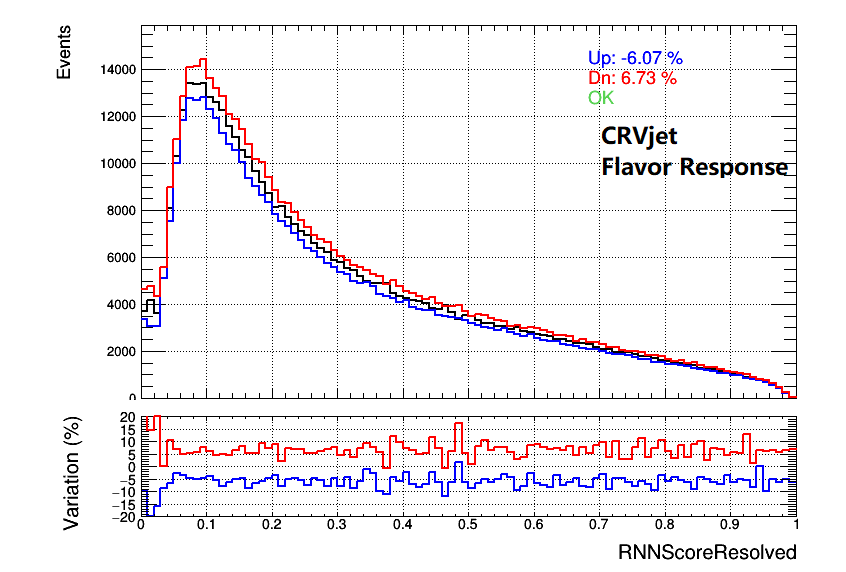
\includegraphics[width=0.4\textwidth]{figures/1lep/FlavorVar/C_0ptag2pjet_0ptv_CRVjet_RNNScoreResolved_SysJET_Flavor_Response.png}}
%%%
%%%        \caption{Impact of Flavour related variations on 1lepton resolved control regions. MC16A events are shown.}
%%%    \label{fig:1LepFlavorVariation}
%%%\end{figure}
%\begin{figure}[ht]
%    \centering
%        \subfigure[Resolved TopCR Flavour Composition]{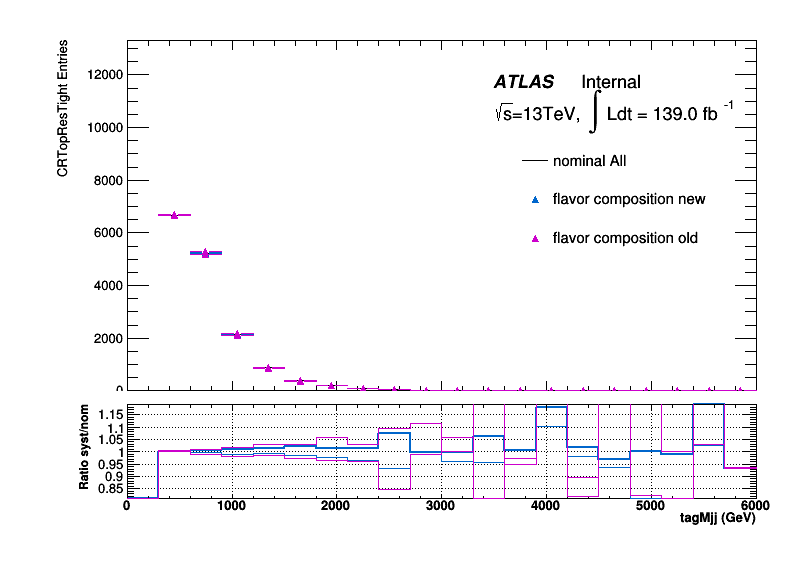
\includegraphics[width=0.4\textwidth]{figures/1lep/FlavorVar/SystFCompCRTopResTight_All_tagMjj.png}}
%        \subfigure[Resolved TopCR Flavour Response]{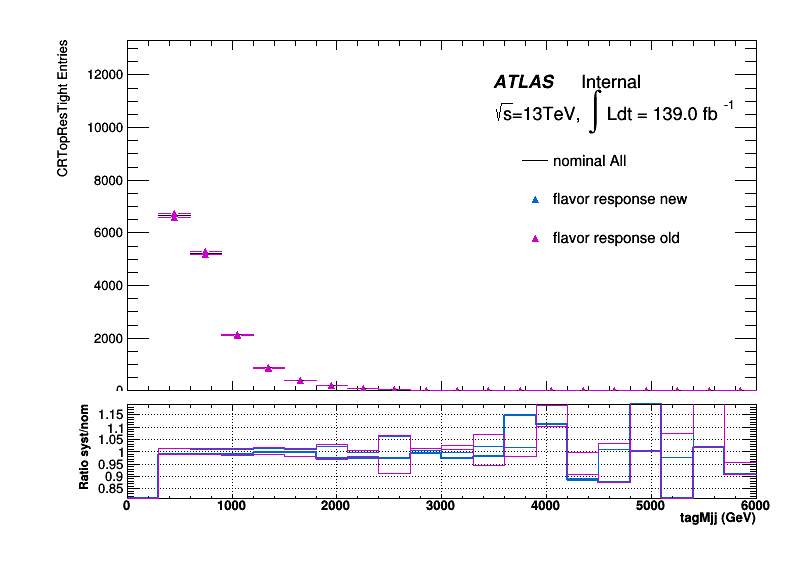
\includegraphics[width=0.4\textwidth]{figures/1lep/FlavorVar/SystFResCRTopResTight_All_tagMjj.png}} \\
%        \subfigure[Resolved WjetsCR Flavour Composition]{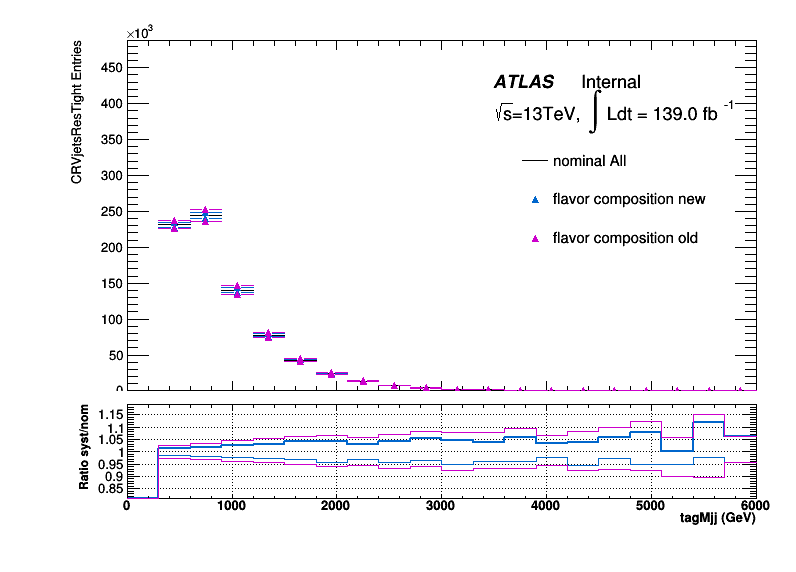
\includegraphics[width=0.4\textwidth]{figures/1lep/FlavorVar/SystFCompCRVjetsResTight_All_tagMjj.png}}
%        \subfigure[Resolved WjetsCR Flavour Reponse]{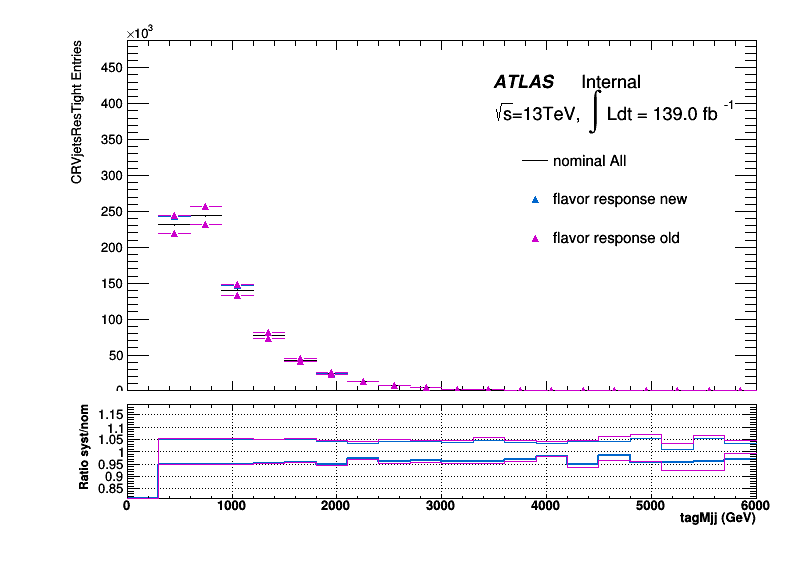
\includegraphics[width=0.4\textwidth]{figures/1lep/FlavorVar/SystFResCRVjetsResTight_All_tagMjj.png}}
%
%        \caption{Comparision between old flavor uncertainties and newly derived flavor uncertainties. Flavor composition uncertainties in particular are greatly reduced.}
%    \label{fig:1LepFlavorVarOldNew}
%\end{figure}



% Gluon fractions as function of pt for 2-lepton channel (nominal)



%%%
\subsection{Tracks uncertainties}
\label{subsec:tracks_uncer}

We incorporate dedicated uncertainties related to track reconstruction, particularly for tracks associated with small-R jets, as outlined in the recommendations on \mbox{\texttt{\href{https://twiki.cern.ch/twiki/bin/viewauth/AtlasProtected/QuarkGluonTagging\#Current_Recommendations}{QuarkGluonTagging}}} and \mbox{\texttt{\href{https://twiki.cern.ch/twiki/bin/view/AtlasProtected/TrackingCPRecsRun2Final\#Track_Systematics_Tools}{TrackingCPRecsRun2Final}}}. 
%Specifically, the ghost-associated track multiplicities of our jets are utilized as inputs to the recurrent layer of the final network.

The procedure in \cite{ATL-PHYS-PUB-2017-009} is used to derive these track multiplicity related uncertainties, of which there are five main components:
\begin{itemize}
    \item fake track efficiency: the uncertainty from the track mis-reconstruction rate;
    \item track efficiency: the uncertainty from the track reconstruction efficiency;
    \item experimental: the uncertainty in charged particle multiplicity, derived as in \cite{CERN-PH-EP-2016-001};
    \item PDF: the theory uncertainty from the parton distribution function;
    \item matrix element: the theory uncertainty from the matrix element calculation;
\end{itemize}
The impacts from these uncertainties are expected to be low.

%%%%%%%%%%%%%%%
%%%We take into account some dedicated uncertainties on the tracks' reconstruction, 
%%%in particular, for the tracks associated to the small-R jets 
%%%\mbox{\texttt{\href{https://twiki.cern.ch/twiki/bin/viewauth/AtlasProtected/QuarkGluonTagging\#Current_Recommendations}{QuarkGluonTagging}}}
%%%\mbox{\texttt{\href{https://twiki.cern.ch/twiki/bin/view/AtlasProtected/TrackingCPRecsRun2Final\#Track_Systematics_Tools}{TrackingCPRecsRun2Final}}}
%%%. 
%%%Indeed, we use the track multiplicities of the ghost associated tracks to our jets as input to the recurrent layer of the final network.
%%%
%%%The procedure in ~\cite{ATL-PHYS-PUB-2017-009}
%%%is used to derive these track multiplicity related uncertainties,
%%%of which there are five main components:
%%%\begin{itemize}
%%%    \item fake track efficiency: uncertainty from track mis-reconstruction rate;
%%%    \item track efficiency: uncertainty from track reconstruction efficiency;
%%%    \item experimental: uncertainty in charged particle multiplicity, derived as in ~\cite{CERN-PH-EP-2016-001};
%%%    \item PDF: theory uncertainty from parton distribution function;
%%%    \item matrix element: theory uncertainty from matrix element calculation;
%%%\end{itemize}
%%%Figures~\ref{fig:1lep_TrackUncCR}, \ref{fig:1lep_TrackUncSR} shows the variations from these sources of
%%%track multiplicity uncertainties for background and signal events in the \olep signal regions.
%%%The impacts from these uncertainties are expected to be low, as they are less than 5\% in the high RNN
%%%bins.

%%%\begin{figure}[ht]
%%%    \centering
%%%        \subfigure[Merged HP SR \ttbar]{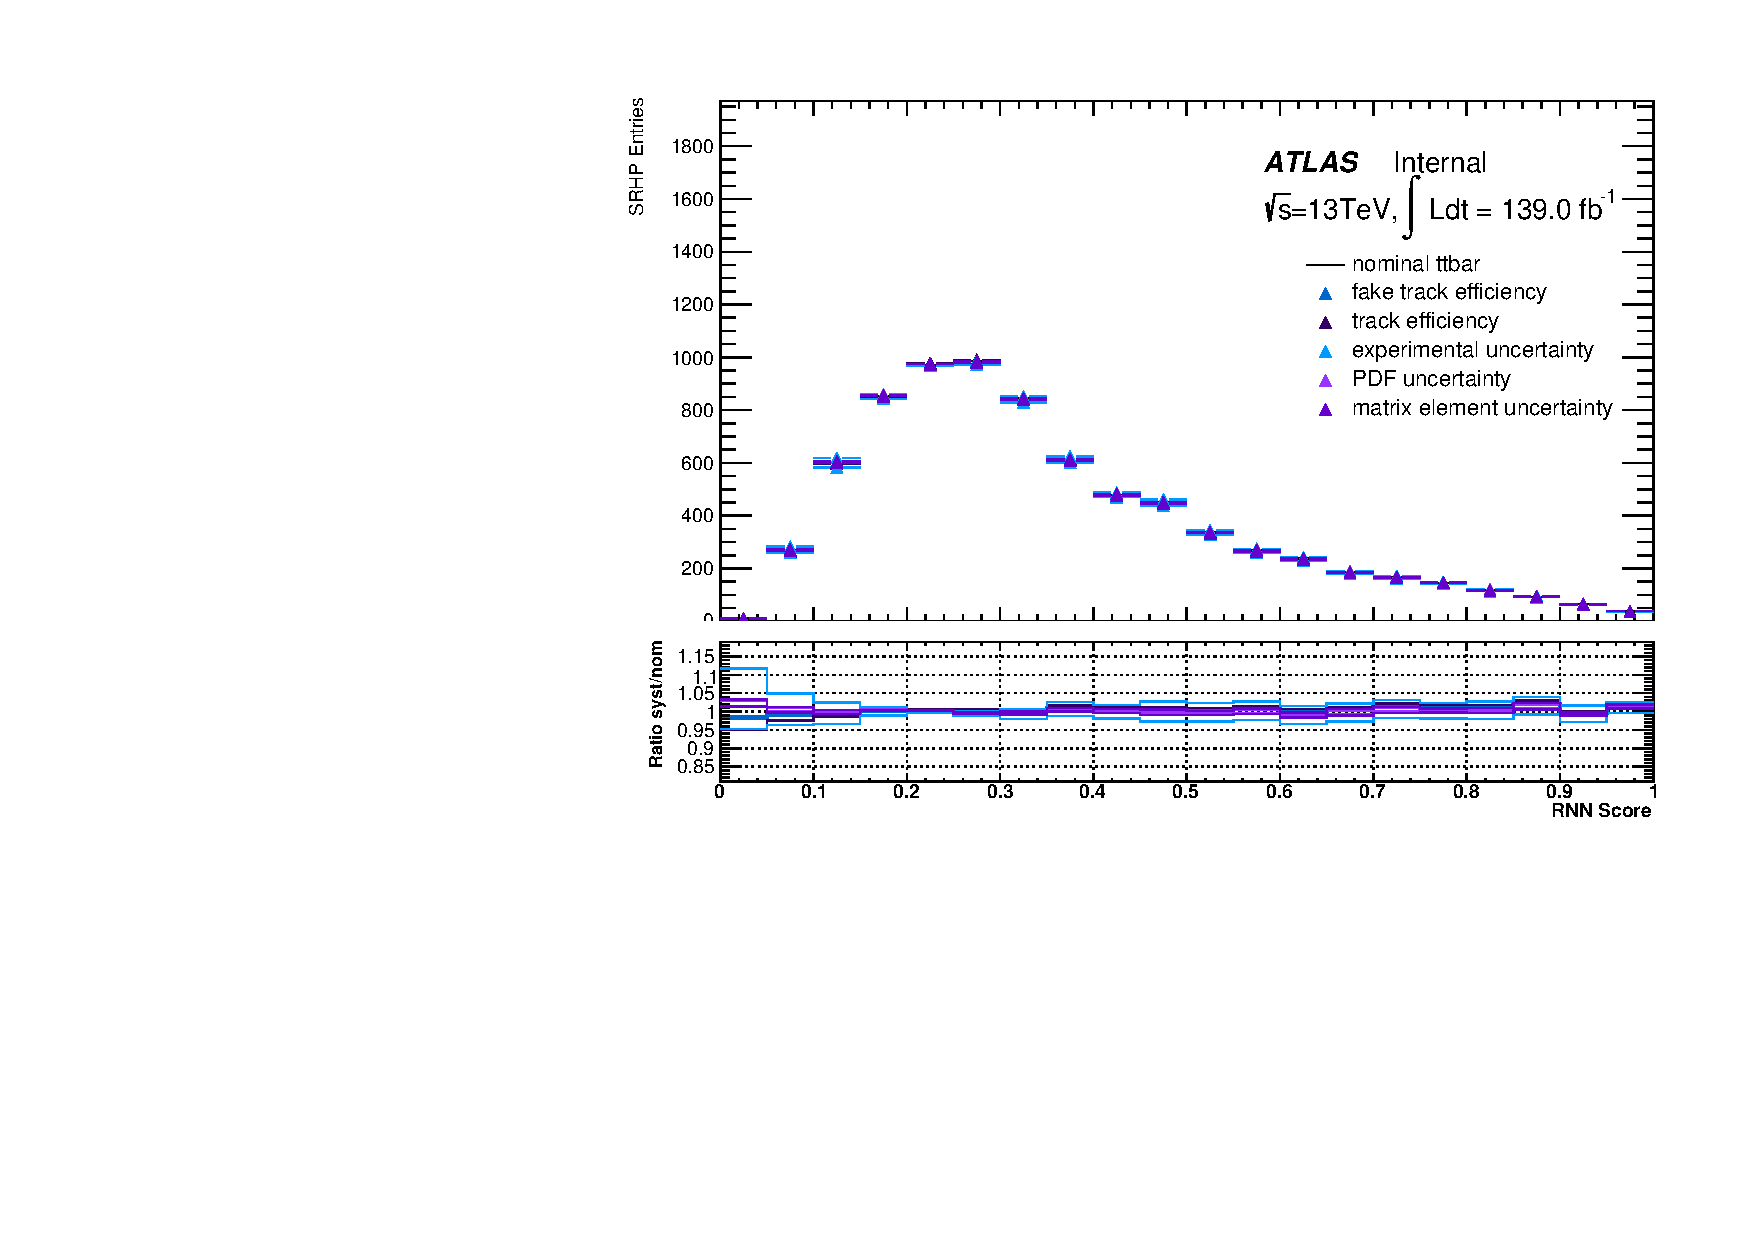
\includegraphics[width=0.45\textwidth]{figures/1lep/TrackSyst/SystQGSRHP_ttbar_RNN.pdf}}
%%%        \subfigure[Merged HP SR W]{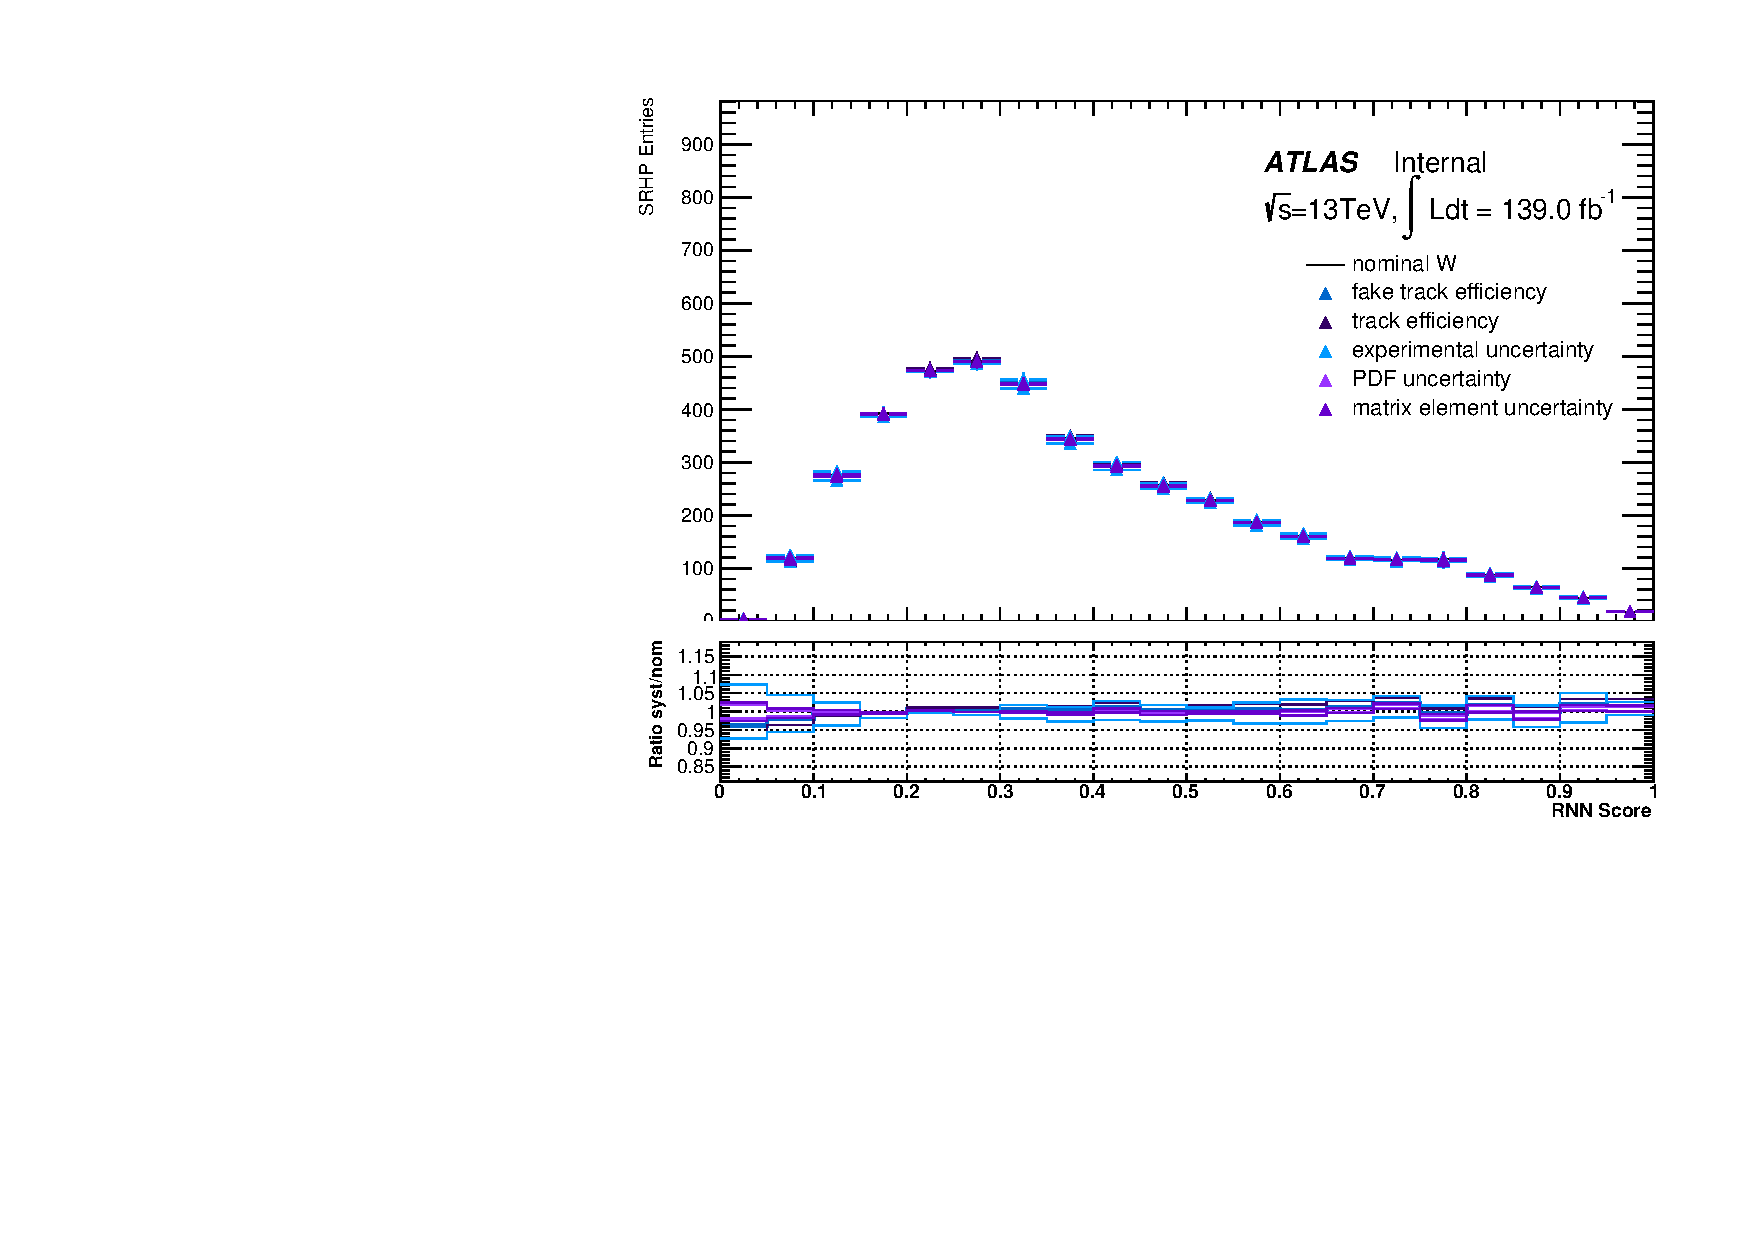
\includegraphics[width=0.45\textwidth]{figures/1lep/TrackSyst/SystQGSRHP_W_RNN.pdf}}
%%%        \subfigure[Merged LP SR \ttbar]{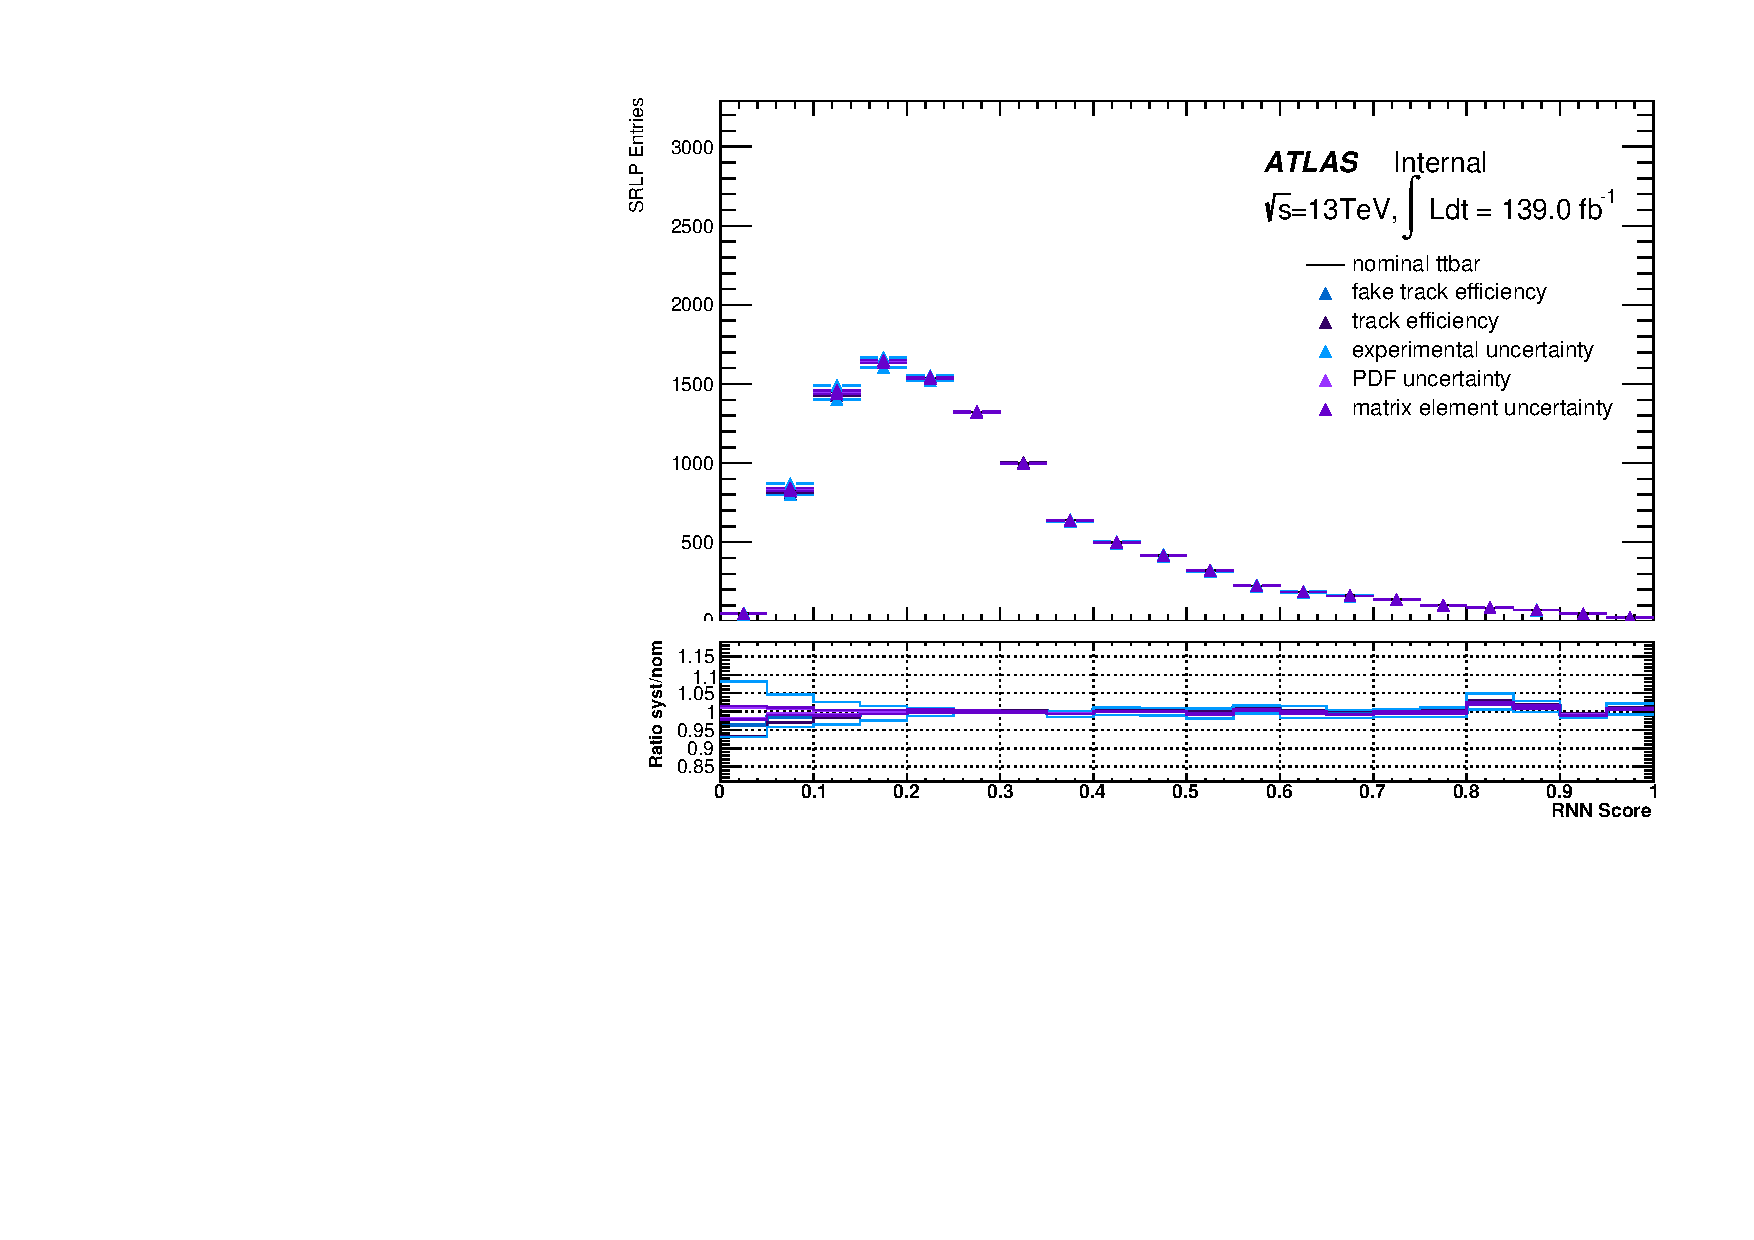
\includegraphics[width=0.45\textwidth]{figures/1lep/TrackSyst/SystQGSRLP_ttbar_RNN.pdf}}
%%%        \subfigure[Merged LP SR W]{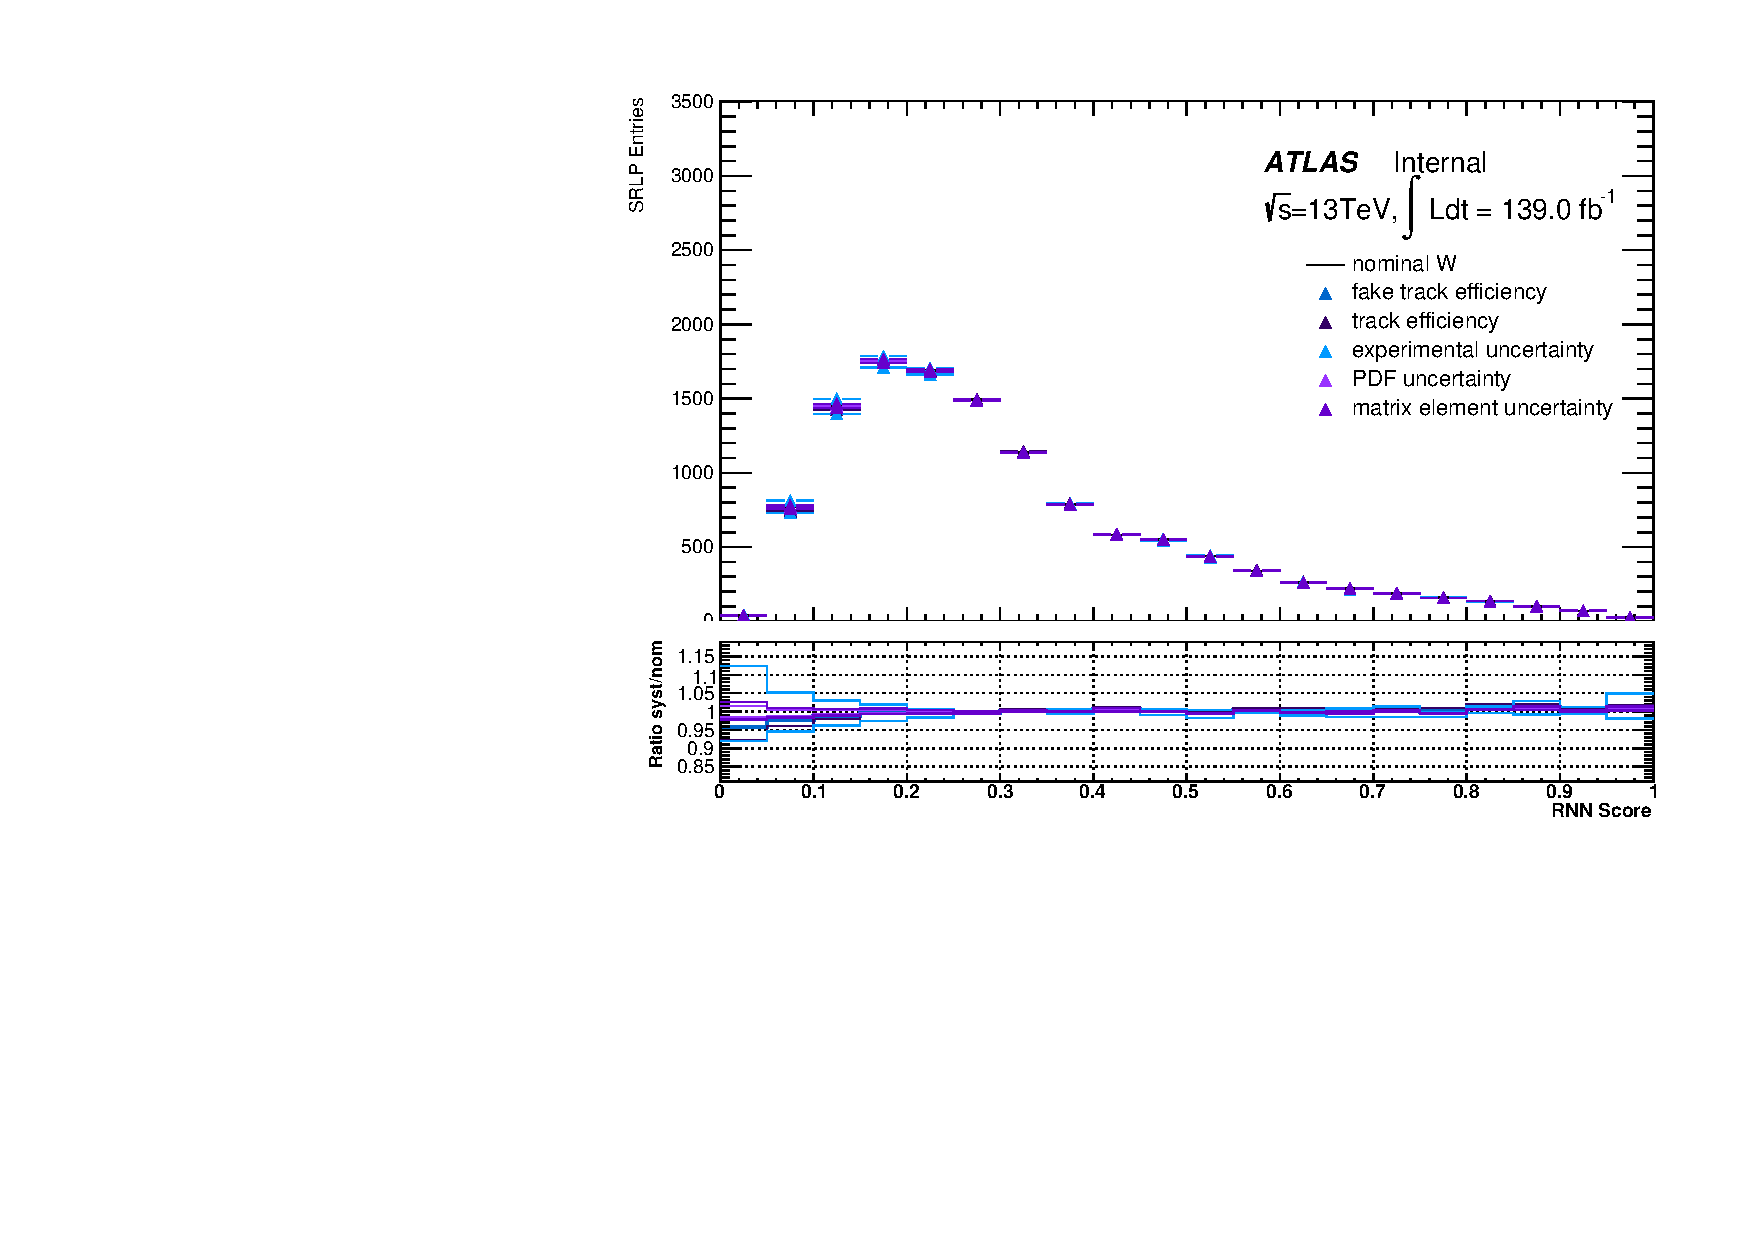
\includegraphics[width=0.45\textwidth]{figures/1lep/TrackSyst/SystQGSRLP_W_RNN.pdf}}
%%%        \subfigure[Resolved SR \ttbar]{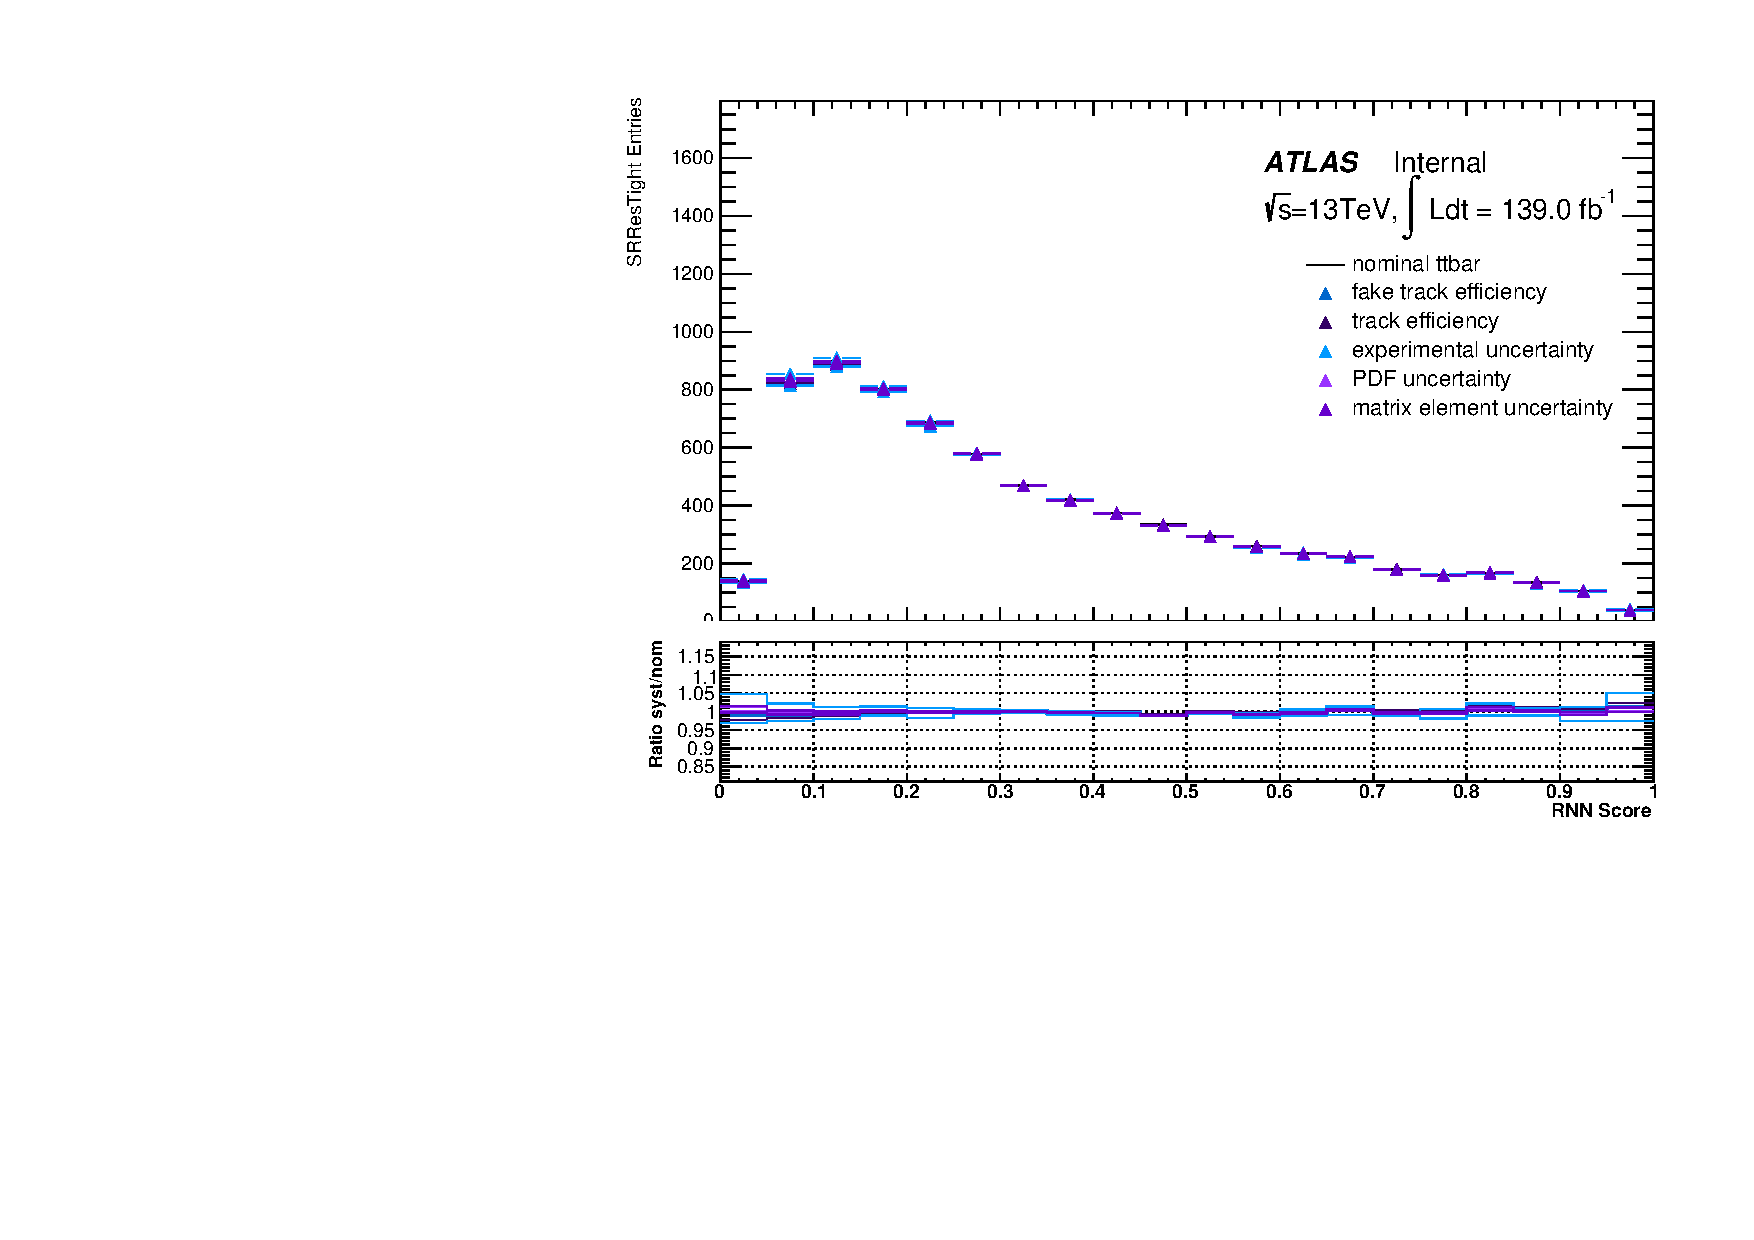
\includegraphics[width=0.45\textwidth]{figures/1lep/TrackSyst/SystQGSRResTight_ttbar_RNN.pdf}}
%%%        \subfigure[Resolved SR W]{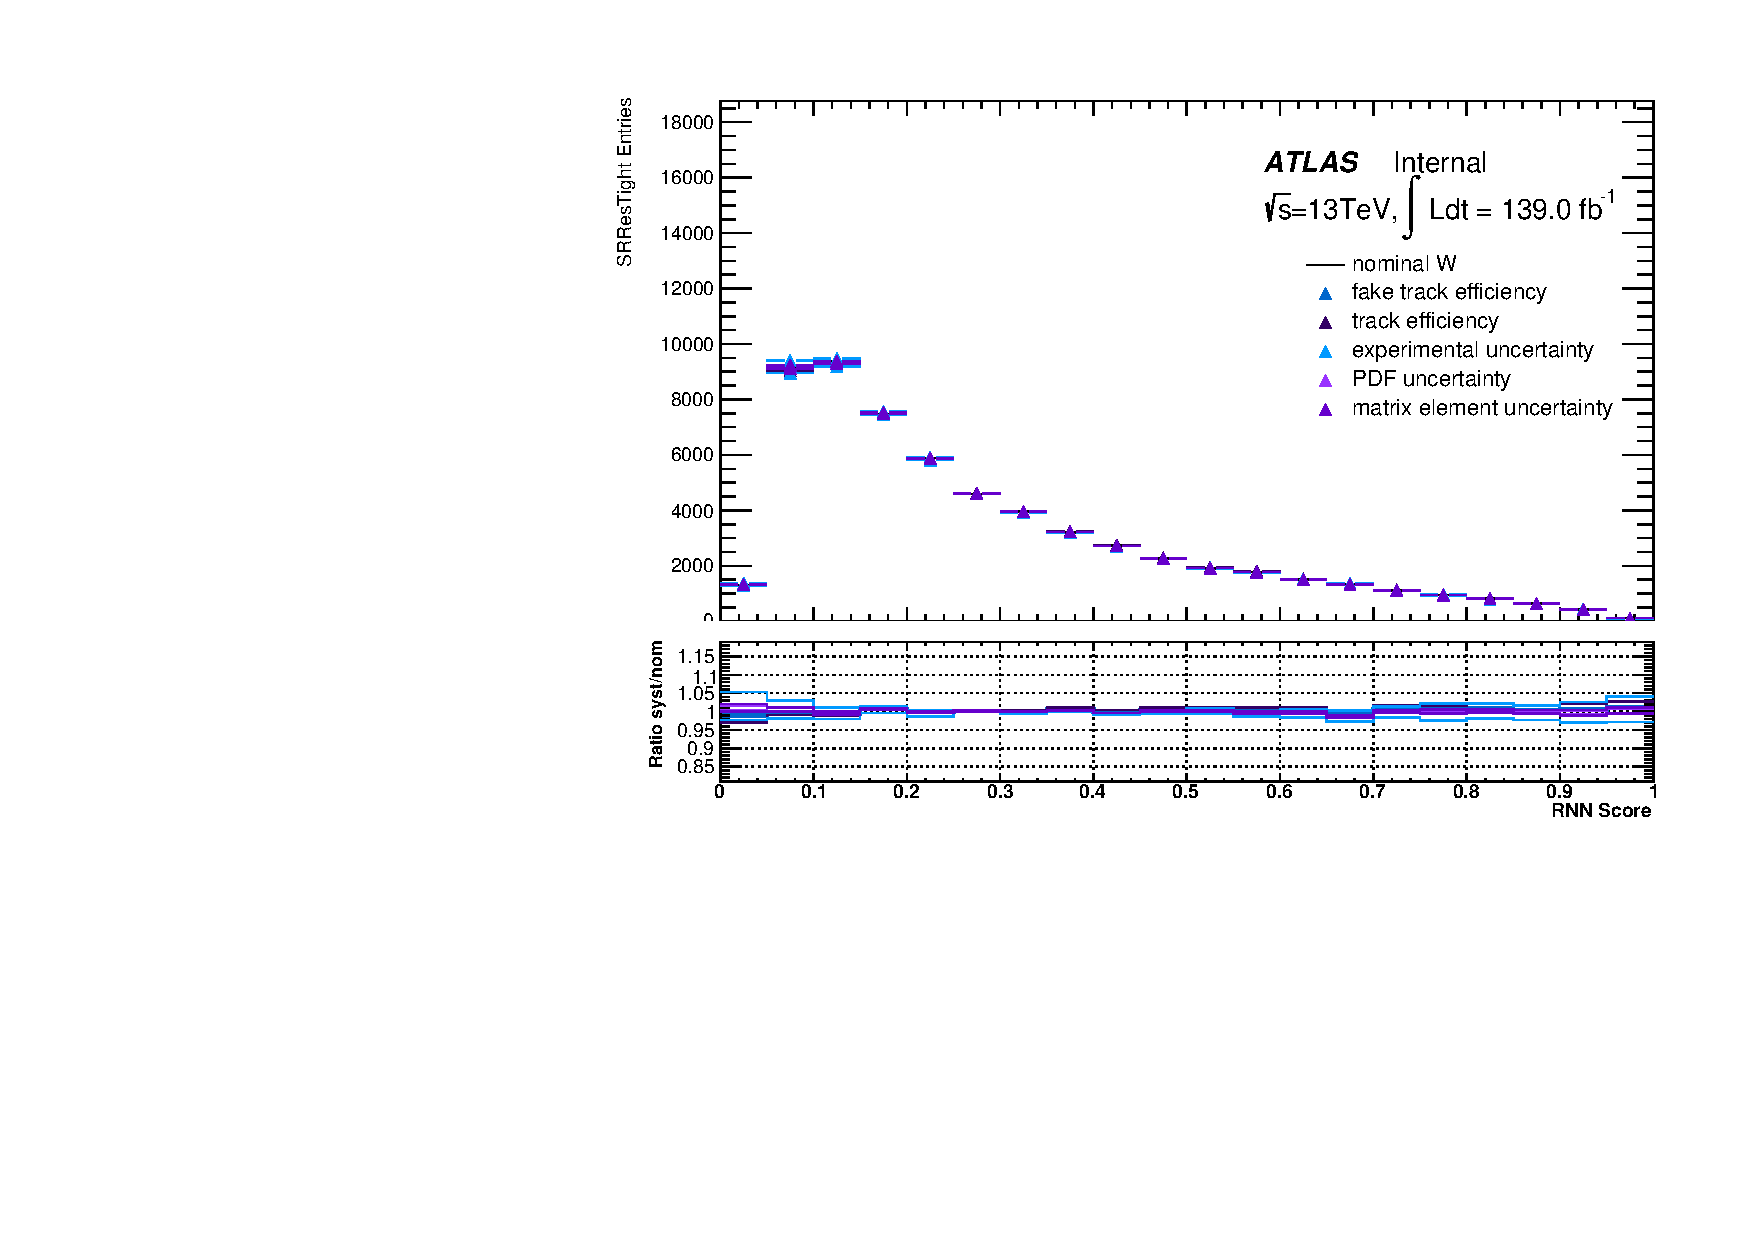
\includegraphics[width=0.45\textwidth]{figures/1lep/TrackSyst/SystQGSRResTight_W_RNN.pdf}}
%%%        \caption{Track multiplicity related uncertainties for \ttbar and \Wjets events in the signal regions. }
%%%    \label{fig:1lep_TrackUncCR}
%%%\end{figure}
%%%
%%%\begin{figure}[ht]
%%%    \centering
%%%        \subfigure[Merged HP SR Signal]{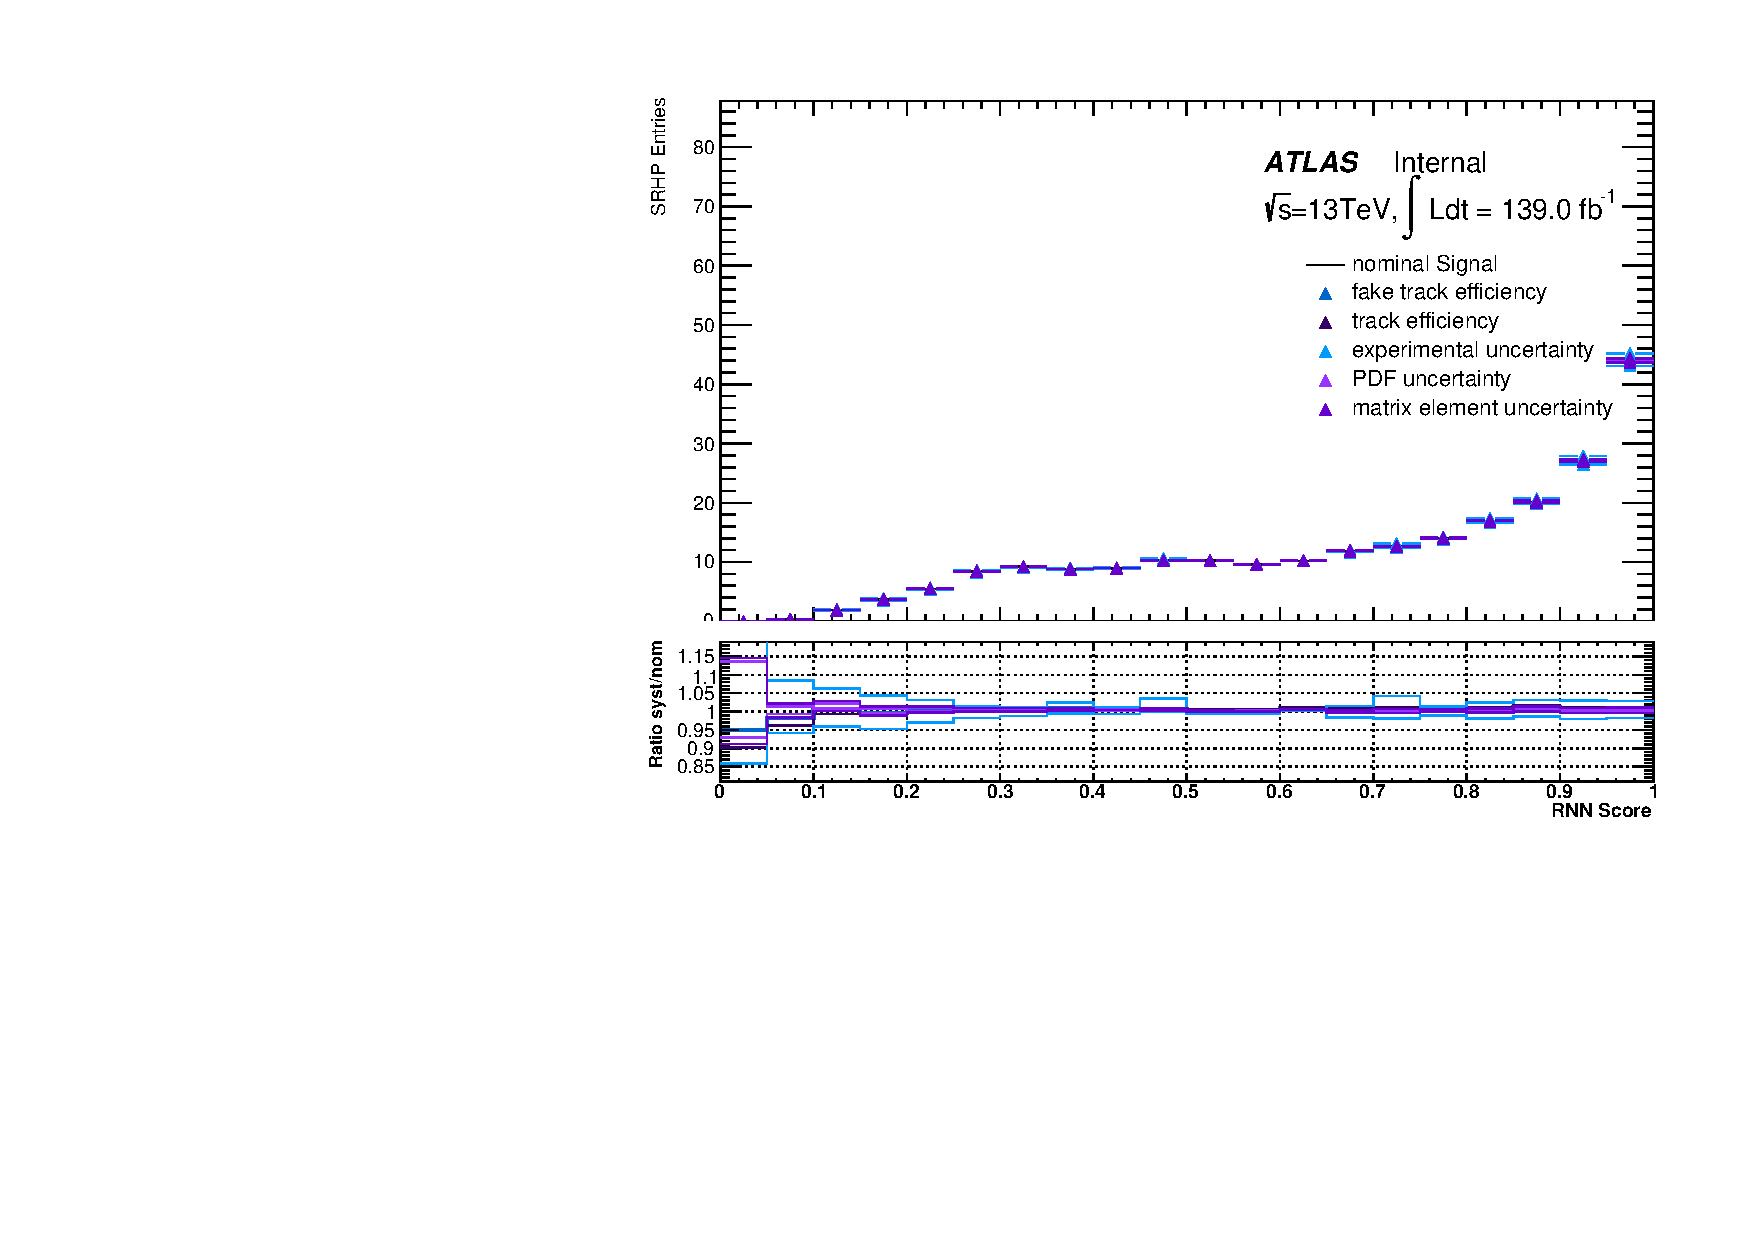
\includegraphics[width=0.45\textwidth]{figures/1lep/TrackSyst/SystQGSRHP_Signal_RNN.pdf}}
%%%        \subfigure[Merged LP SR Signal]{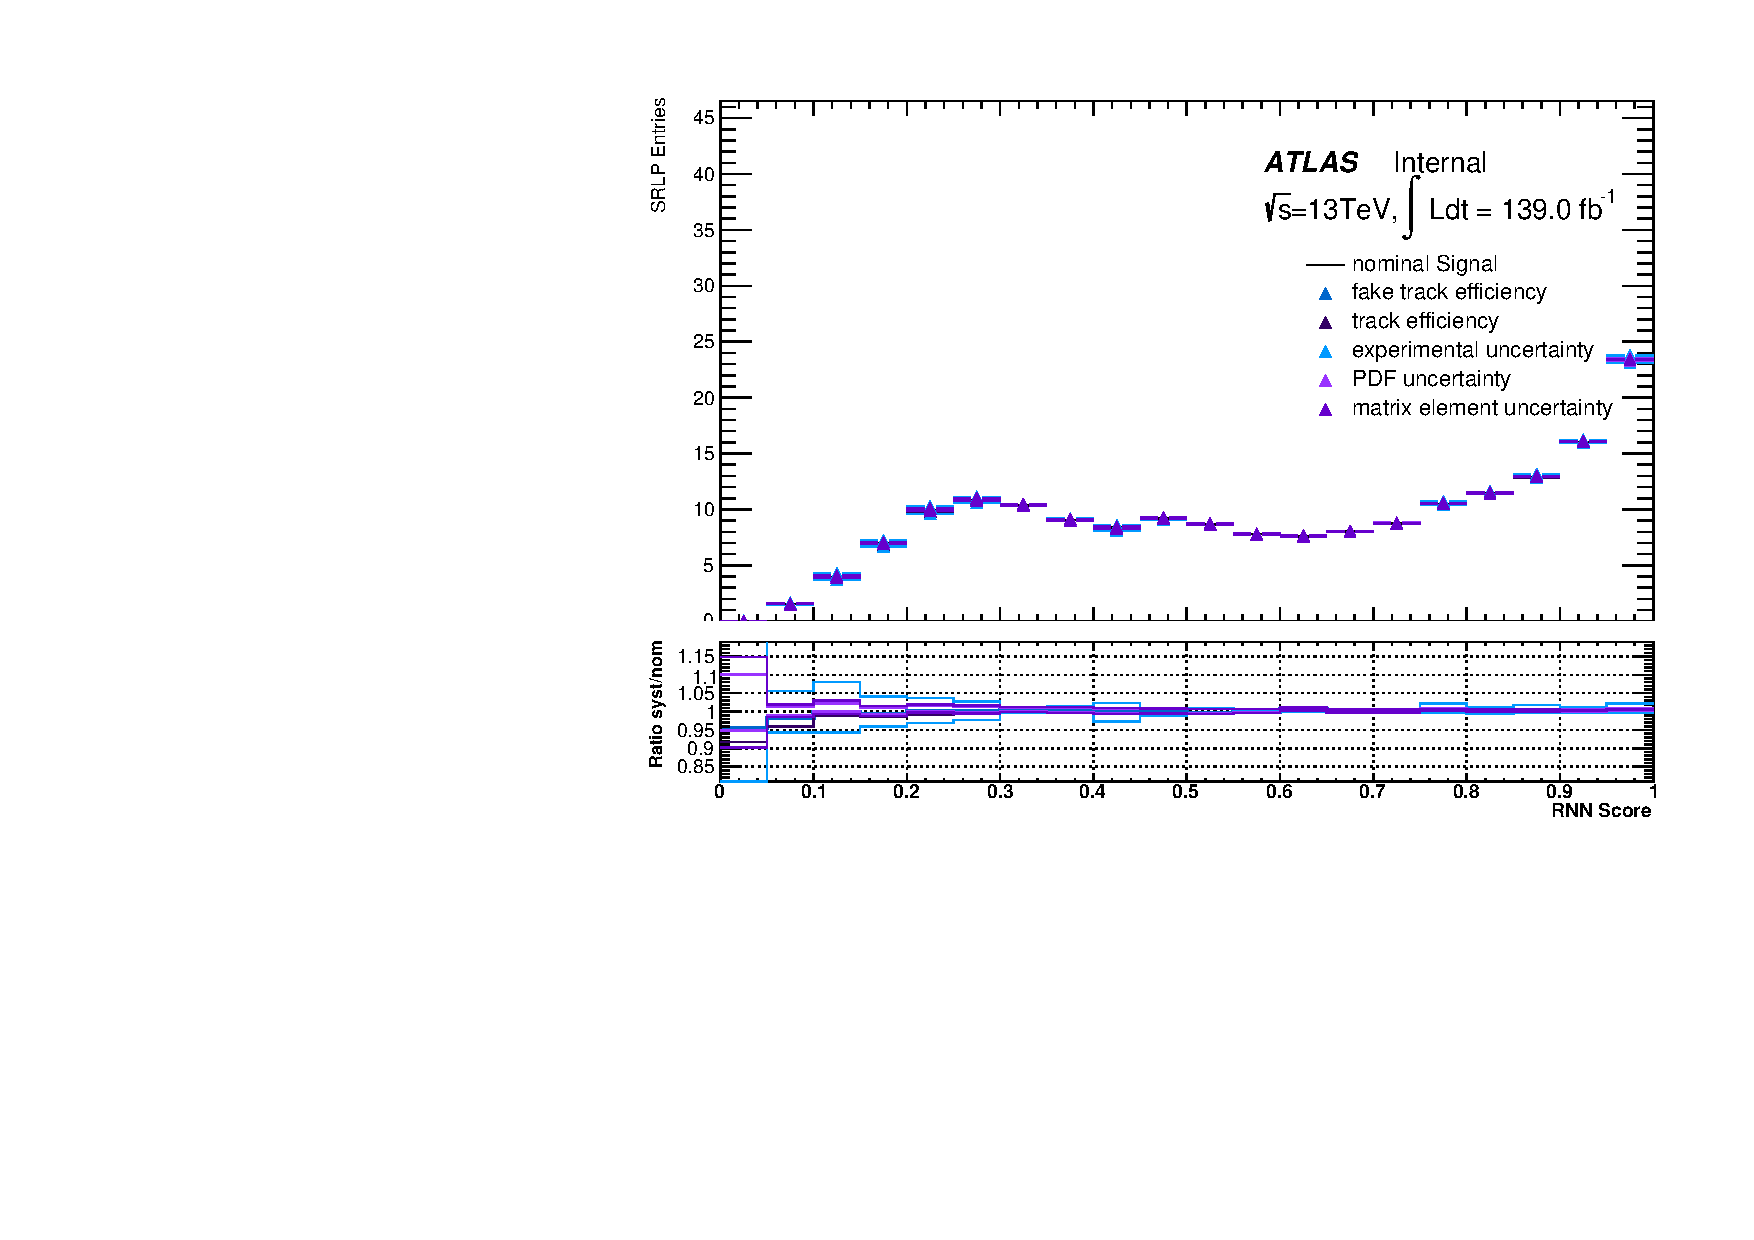
\includegraphics[width=0.45\textwidth]{figures/1lep/TrackSyst/SystQGSRLP_Signal_RNN.pdf}}
%%%        \subfigure[Resolved SR Signal]{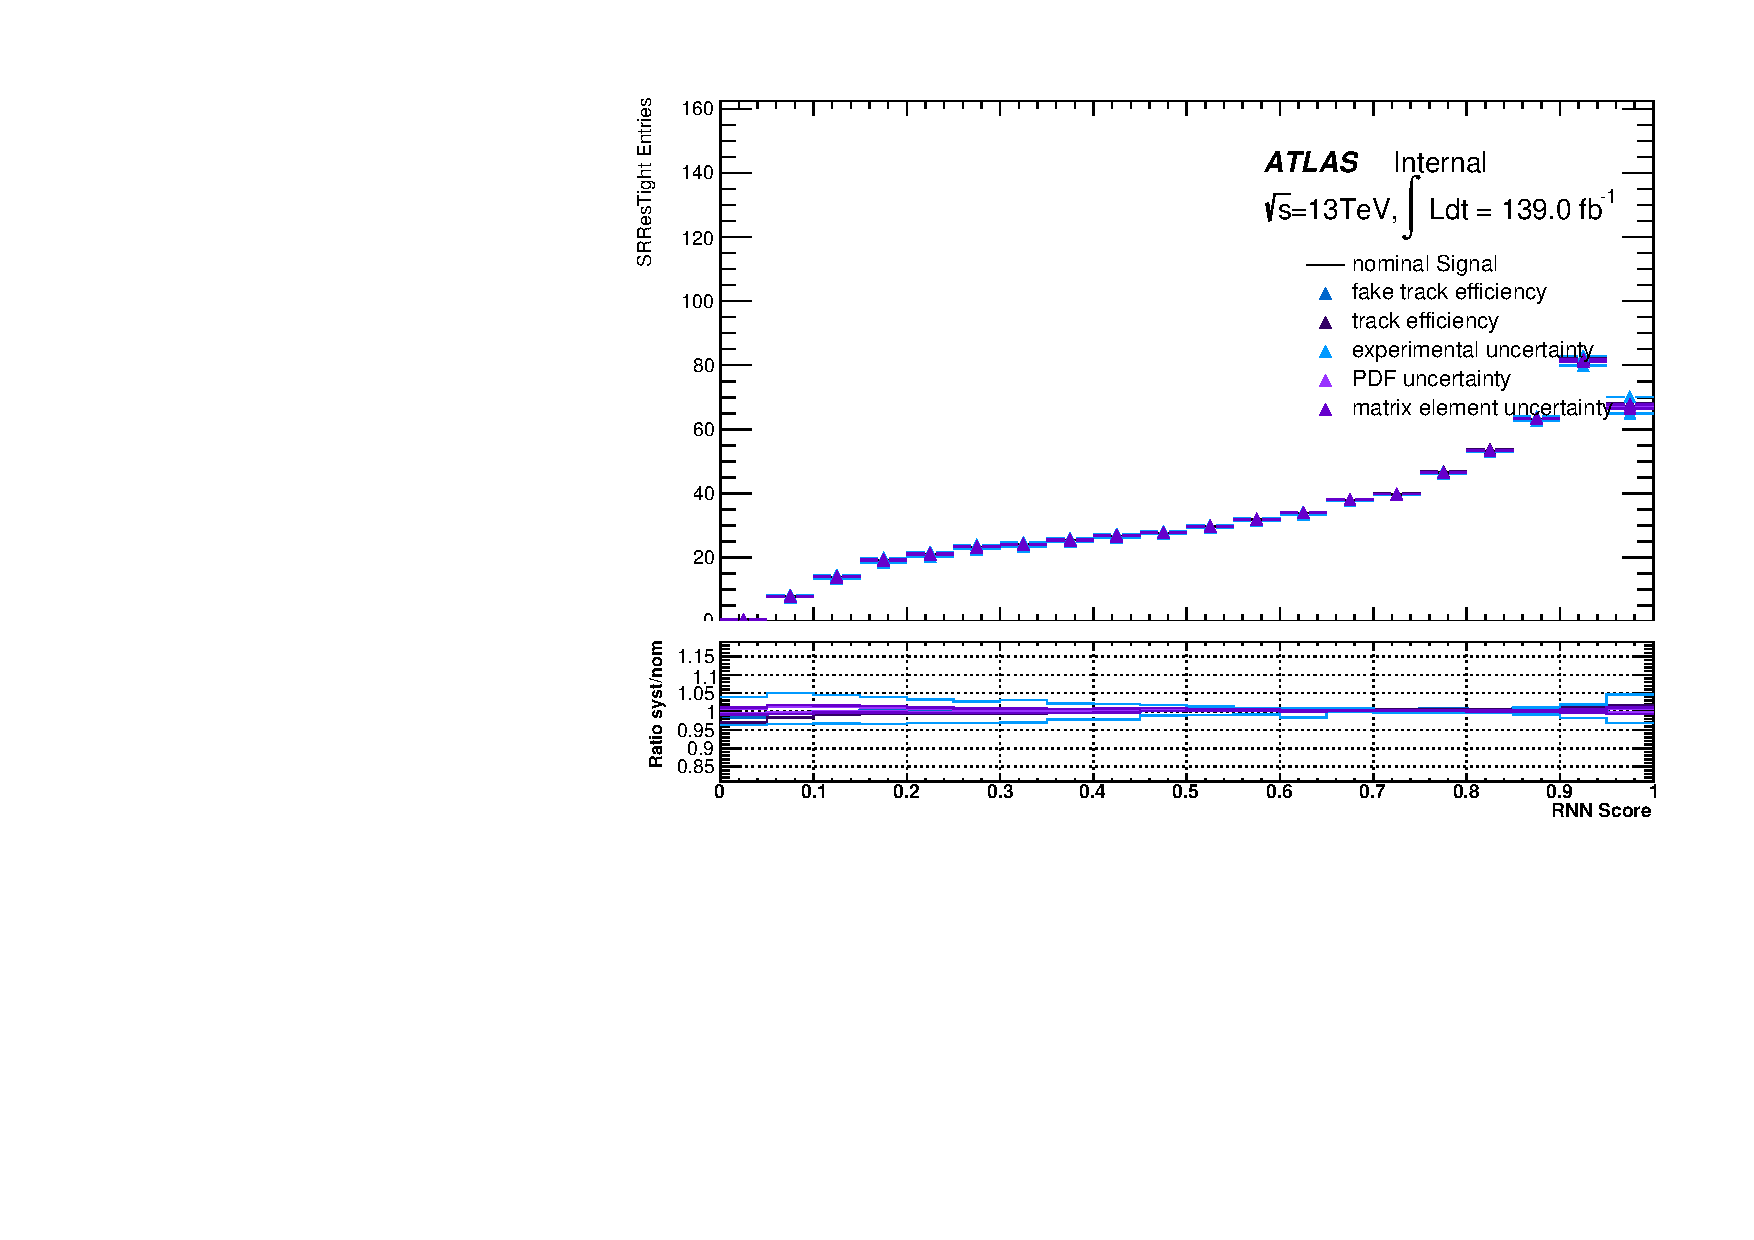
\includegraphics[width=0.45\textwidth]{figures/1lep/TrackSyst/SystQGSRResTight_Signal_RNN.pdf}}
%%%        \caption{Track multiplicity related uncertainties for signal events in the signal regions. }
%%%    \label{fig:1lep_TrackUncSR}
%%%\end{figure}


%both from quick statistics test 
%both from past studies in the VV semi-leptonic resonant search \cite{Bachas:2646593}.



%
\clearpage
\section{Background Uncertainties}
%\clearpage
%\subsection{Background Uncertainties}
\label{subsec:bkg_uncer}

%%%	
Several systematic uncertainties associated with the modeling of backgrounds have been assessed. These uncertainties include a shape systematic related to the discriminant used in the analysis and a normalization systematic for predictions derived solely from simulations.
The complete list of the alternative samples utilized to derive these background uncertainties is provided in the Tables
\ref{tabular:mc_samples_alt_Wenujets}-\ref{tabular:mc_samples_alt_ttbar}.

%%% alternative bkg samples
\begin{table}[p]
\caption{$W \to e\nu$+jets alternative samples used in the analysis. The dataset ID, MC generator, production cross section, filter efficiency and total number of generated events are shown.}
\label{tabular:mc_samples_alt_Wenujets}
\begin{footnotesize}
\begin{center}
\begin{tabular}{c|l|c|c|c}
  \hline
  DS ID & Name & $\sigma\times\text{BR}$ [pb] & k-factor & $\epsilon_{\text{filter}}$ \\ \hline
363600  & MGPy8EG\_N30NLO\_Wenu\_Ht0\_70\_CVetoBVeto            & 16719.0                      & 1.12      & 8.38E+03 \\
363601  & MGPy8EG\_N30NLO\_Wenu\_Ht0\_70\_CFilterBVeto          & 16720.0                      & 1.12      & 1.38E+03 \\
363602  & MGPy8EG\_N30NLO\_Wenu\_Ht0\_70\_BFilter               & 16717.0                      & 1.12      & 2.42E+02 \\
363603  & MGPy8EG\_N30NLO\_Wenu\_Ht70\_140\_CVetoBVeto          & 755.1                        & 1.12      & 7.12E+03 \\
363604  & MGPy8EG\_N30NLO\_Wenu\_Ht70\_140\_CFilterBVeto        & 755.77                       & 1.12      & 2.40E+03 \\
363605  & MGPy8EG\_N30NLO\_Wenu\_Ht70\_140\_BFilter             & 755.73                       & 1.12      & 4.83E+02 \\
363606  & MGPy8EG\_N30NLO\_Wenu\_Ht140\_280\_CVetoBVeto         & 318.96                       & 1.12      & 6.66E+03 \\
363607  & MGPy8EG\_N30NLO\_Wenu\_Ht140\_280\_CFilterBVeto       & 319.93                       & 1.12      & 2.64E+03 \\
363608  & MGPy8EG\_N30NLO\_Wenu\_Ht140\_280\_BFilter            & 319.45                       & 1.12      & 6.94E+02 \\
363609  & MGPy8EG\_N30NLO\_Wenu\_Ht280\_500\_CVetoBVeto         & 73.528                       & 1.12      & 6.19E+03 \\
363610  & MGPy8EG\_N30NLO\_Wenu\_Ht280\_500\_CFilterBVeto       & 73.562                       & 1.12      & 2.85E+03 \\
363611  & MGPy8EG\_N30NLO\_Wenu\_Ht280\_500\_BFilter            & 73.556                       & 1.12      & 9.52E+02 \\
363612  & MGPy8EG\_N30NLO\_Wenu\_Ht500\_700\_CVetoBVeto         & 11.529                       & 1.12      & 5.87E+03 \\
363613  & MGPy8EG\_N30NLO\_Wenu\_Ht500\_700\_CFilterBVeto       & 11.517                       & 1.12      & 2.98E+03 \\
363614  & MGPy8EG\_N30NLO\_Wenu\_Ht500\_700\_BFilter            & 11.51                        & 1.12      & 1.15E+03 \\
363615  & MGPy8EG\_N30NLO\_Wenu\_Ht700\_1000\_CVetoBVeto        & 40.158                       & 1.12      & 5.66E+03 \\
363616  & MGPy8EG\_N30NLO\_Wenu\_Ht700\_1000\_CFilterBVeto      & 4.014                        & 1.12      & 3.04E+03 \\
363617  & MGPy8EG\_N30NLO\_Wenu\_Ht700\_1000\_BFilter           & 40.123                       & 1.12      & 1.28E+03 \\
363618  & MGPy8EG\_N30NLO\_Wenu\_Ht1000\_2000\_CVetoBVeto       & 13.243                       & 1.12      & 5.48E+03 \\
363619  & MGPy8EG\_N30NLO\_Wenu\_Ht1000\_2000\_CFilterBVeto     & 13.286                       & 1.12      & 3.08E+03 \\
363620  & MGPy8EG\_N30NLO\_Wenu\_Ht1000\_2000\_BFilter          & 1.326                        & 1.12      & 1.43E+03 \\
363621  & MGPy8EG\_N30NLO\_Wenu\_Ht2000\_E\_CMS\_CVetoBVeto      & 0.042294                     & 1.12      & 5.24E+03 \\
363622  & MGPy8EG\_N30NLO\_Wenu\_Ht2000\_E\_CMS\_CFilterBVeto    & 0.041884                     & 1.12      & 3.17E+03 \\
363623  & MGPy8EG\_N30NLO\_Wenu\_Ht2000\_E\_CMS\_BFilter         & 0.047382                     & 1.12      & 1.51E+03 \\
\hline
\end{tabular}
\end{center}
\end{footnotesize}
\end{table}

\begin{table}[p]
\caption{$W \to \mu\nu$+jets alternative samples used in the analysis. The dataset ID, MC generator, production cross section, filter efficiency and total number of generated events are shown.}
\label{tabular:mc_samples_alt_Wmunujets}
\begin{footnotesize}
\begin{center}
\begin{tabular}{c|l|c|c|c}
  \hline
  DS ID & Name & $\sigma\times\text{BR}$ [pb] & k-factor & $\epsilon_{\text{filter}}$ \\ \hline
363624  & MGPy8EG\_N30NLO\_Wmunu\_Ht0\_70\_CVetoBVeto         & 16720.0                    &  1.12   &       8.38E+03        \\
363625  & MGPy8EG\_N30NLO\_Wmunu\_Ht0\_70\_CFilterBVeto       & 16717.0                    &  1.12   &       1.38E+03        \\
363626  & MGPy8EG\_N30NLO\_Wmunu\_Ht0\_70\_BFilter            & 16719.0                    &  1.12   &       2.42E+02        \\
363627  & MGPy8EG\_N30NLO\_Wmunu\_Ht70\_140\_CVetoBVeto       & 755.19                     &  1.12   &       7.12E+03        \\
363628  & MGPy8EG\_N30NLO\_Wmunu\_Ht70\_140\_CFilterBVeto     & 755.62                     &  1.12   &       2.40E+03        \\
363629  & MGPy8EG\_N30NLO\_Wmunu\_Ht70\_140\_BFilter          & 755.77                     &  1.12   &       4.83E+02        \\
363630  & MGPy8EG\_N30NLO\_Wmunu\_Ht140\_280\_CVetoBVeto      & 318.83                     &  1.12   &       6.66E+03        \\
363631  & MGPy8EG\_N30NLO\_Wmunu\_Ht140\_280\_CFilterBVeto    & 319.89                     &  1.12   &       2.64E+03        \\
363632  & MGPy8EG\_N30NLO\_Wmunu\_Ht140\_280\_BFilter         & 319.41                     &  1.12   &       6.94E+02        \\
363633  & MGPy8EG\_N30NLO\_Wmunu\_Ht280\_500\_CVetoBVeto      & 73.585                     &  1.12   &       6.19E+03        \\
363634  & MGPy8EG\_N30NLO\_Wmunu\_Ht280\_500\_CFilterBVeto    & 73.548                     &  1.12   &       2.85E+03        \\
363635  & MGPy8EG\_N30NLO\_Wmunu\_Ht280\_500\_BFilter         & 73.569                     &  1.12   &       9.52E+02        \\
363636  & MGPy8EG\_N30NLO\_Wmunu\_Ht500\_700\_CVetoBVeto      & 11.522                     &  1.12   &       5.86E+03        \\
363637  & MGPy8EG\_N30NLO\_Wmunu\_Ht500\_700\_CFilterBVeto    & 11.524                     &  1.12   &       2.96E+03        \\
363638  & MGPy8EG\_N30NLO\_Wmunu\_Ht500\_700\_BFilter         & 11.522                     &  1.12   &       1.16E+03        \\
363639  & MGPy8EG\_N30NLO\_Wmunu\_Ht700\_1000\_CVetoBVeto     & 40.194                     &  1.12   &       5.67E+03        \\
363640  & MGPy8EG\_N30NLO\_Wmunu\_Ht700\_1000\_CFilterBVeto   & 40.252                     &  1.12   &       3.05E+03        \\
363641  & MGPy8EG\_N30NLO\_Wmunu\_Ht700\_1000\_BFilter        & 40.139                     &  1.12   &       1.28E+03        \\
363642  & MGPy8EG\_N30NLO\_Wmunu\_Ht1000\_2000\_CVetoBVeto    & 13.262                     &  1.12   &       5.45E+03        \\
363643  & MGPy8EG\_N30NLO\_Wmunu\_Ht1000\_2000\_CFilterBVeto  & 13.215                     &  1.12   &       3.08E+03        \\
363644  & MGPy8EG\_N30NLO\_Wmunu\_Ht1000\_2000\_BFilter       & 13.287                     &  1.12   &       1.44E+03        \\
363645  & MGPy8EG\_N30NLO\_Wmunu\_Ht2000\_E\_CMS\_CVetoBVeto   & 0.041697                   &  1.12   &       5.20E+03        \\
363646  & MGPy8EG\_N30NLO\_Wmunu\_Ht2000\_E\_CMS\_CFilterBVeto & 0.042199                   &  1.12   &       3.17E+03        \\
363647  & MGPy8EG\_N30NLO\_Wmunu\_Ht2000\_E\_CMS\_BFilter      & 0.042049                   &  1.12   &       1.59E+03        \\
\hline
\end{tabular}
\end{center}
\end{footnotesize}
\end{table}

\begin{table}[p]
\caption{$W \to \tau\nu$+jets alternative samples used in the analysis. The dataset ID, MC generator, production cross section, filter efficiency and total number of generated events are shown.}
\label{tabular:mc_samples_alt_Wtaunujets}
\begin{footnotesize}
\begin{center}
\begin{tabular}{c|l|c|c|c}
  \hline
  DS ID & Name & $\sigma\times\text{BR}$ [pb] & k-factor & $\epsilon_{\text{filter}}$ \\ \hline
363648  & MGPy8EG\_N30NLO\_Wtaunu\_Ht0\_70\_CVetoBVeto        & 16702.0                    &  1.12   &       8.38E+03        \\
363649  & MGPy8EG\_N30NLO\_Wtaunu\_Ht0\_70\_CFilterBVeto      & 16702.0                    &  1.12   &       1.38E+03        \\
363650  & MGPy8EG\_N30NLO\_Wtaunu\_Ht0\_70\_BFilter           & 16702.0                    &  1.12   &       2.42E+02        \\
363651  & MGPy8EG\_N30NLO\_Wtaunu\_Ht70\_140\_CVetoBVeto      & 754.91                     &  1.12   &       7.12E+03        \\
363652  & MGPy8EG\_N30NLO\_Wtaunu\_Ht70\_140\_CFilterBVeto    & 755.3                      &  1.12   &       2.39E+03        \\
363653  & MGPy8EG\_N30NLO\_Wtaunu\_Ht70\_140\_BFilter         & 755.14                     &  1.12   &       4.85E+02        \\
363654  & MGPy8EG\_N30NLO\_Wtaunu\_Ht140\_280\_CVetoBVeto     & 315.31                     &  1.12   &       6.67E+03        \\
363655  & MGPy8EG\_N30NLO\_Wtaunu\_Ht140\_280\_CFilterBVeto   & 316.05                     &  1.12   &       2.64E+03        \\
363656  & MGPy8EG\_N30NLO\_Wtaunu\_Ht140\_280\_BFilter        & 315.64                     &  1.12   &       6.93E+02        \\
363657  & MGPy8EG\_N30NLO\_Wtaunu\_Ht280\_500\_CVetoBVeto     & 72.275                     &  1.12   &       6.22E+03        \\
363658  & MGPy8EG\_N30NLO\_Wtaunu\_Ht280\_500\_CFilterBVeto   & 72.19                      &  1.12   &       2.85E+03        \\
363659  & MGPy8EG\_N30NLO\_Wtaunu\_Ht280\_500\_BFilter        & 72.226                     &  1.12   &       9.52E+02        \\
363660  & MGPy8EG\_N30NLO\_Wtaunu\_Ht500\_700\_CVetoBVeto     & 11.44                      &  1.12   &       5.88E+03        \\
363661  & MGPy8EG\_N30NLO\_Wtaunu\_Ht500\_700\_CFilterBVeto   & 11.463                     &  1.12   &       2.97E+03        \\
363662  & MGPy8EG\_N30NLO\_Wtaunu\_Ht500\_700\_BFilter        & 11.459                     &  1.12   &       1.16E+03        \\
363663  & MGPy8EG\_N30NLO\_Wtaunu\_Ht700\_1000\_CVetoBVeto    & 40.265                     &  1.12   &       5.67E+03        \\
363664  & MGPy8EG\_N30NLO\_Wtaunu\_Ht700\_1000\_CFilterBVeto  & 4.027                      &  1.12   &       3.03E+03        \\
363665  & MGPy8EG\_N30NLO\_Wtaunu\_Ht700\_1000\_BFilter       & 40.283                     &  1.12   &       1.30E+03        \\
363666  & MGPy8EG\_N30NLO\_Wtaunu\_Ht1000\_2000\_CVetoBVeto   & 13.264                     &  1.12   &       5.46E+03        \\
363667  & MGPy8EG\_N30NLO\_Wtaunu\_Ht1000\_2000\_CFilterBVeto & 13.205                     &  1.12   &       3.12E+03        \\
363668  & MGPy8EG\_N30NLO\_Wtaunu\_Ht1000\_2000\_BFilter      & 13.222                     &  1.12   &       1.43E+03        \\
363669  & MGPy8EG\_N30NLO\_Wtaunu\_Ht2000\_E\_CMS\_CVetoBVeto  & 0.043501                   &  1.12   &       5.21E+03        \\
363670  & MGPy8EG\_N30NLO\_Wtaunu\_Ht2000\_E\_CMS\_CFilterBVeto  &                          0.042721  &       1.12            & 3.18E+03 \\
363671  & MGPy8EG\_N30NLO\_Wtaunu\_Ht2000\_E\_CMS\_BFilter       &                          0.042683  &       1.12            & 1.66E+03 \\
\hline
\end{tabular}
\end{center}
\end{footnotesize}
\end{table}

\begin{table}[p]
\caption{$Z \to ee$+jets alternative samples used in the analysis. The dataset ID, MC generator, production cross section, filter efficiency and total number of generated events are shown.}
\label{tabular:mc_samples_alt_Zeejets}
\begin{footnotesize}
\begin{center}
\begin{tabular}{c|l|c|c|c}
  \hline
  DS ID & Name & $\sigma\times\text{BR}$ [pb] & k-factor & $\epsilon_{\text{filter}}$ \\ \hline
363147  & MGPy8EG\_N30NLO\_Zee\_Ht0\_70\_CVetoBVeto  &        1719.7                       &  1.141  &       0.83292 \\
363148  & MGPy8EG\_N30NLO\_Zee\_Ht0\_70\_CFilterBVeto         &                            1719.4    &       1.141   &       0.10775 \\
363149  & MGPy8EG\_N30NLO\_Zee\_Ht0\_70\_BFilter              &                            1719.4    &       1.141   &       0.059156 \\
363150  & MGPy8EG\_N30NLO\_Zee\_Ht70\_140\_CVetoBVeto         &                            85.105    &       1.141   &       0.71754  \\
363151  & MGPy8EG\_N30NLO\_Zee\_Ht70\_140\_CFilterBVeto       &                            85.041    &       1.141   &       0.17377  \\
363152  & MGPy8EG\_N30NLO\_Zee\_Ht70\_140\_BFilter            &                            85.175    &       1.141   &       0.10763  \\
363153  & MGPy8EG\_N30NLO\_Zee\_Ht140\_280\_CVetoBVeto        &                            36.005    &       1.141   &       0.67279  \\
363154  & MGPy8EG\_N30NLO\_Zee\_Ht140\_280\_CFilterBVeto      &                            36.028    &       1.141   &       0.19996  \\
363155  & MGPy8EG\_N30NLO\_Zee\_Ht140\_280\_BFilter           &                            36.06     &       1.141   &       0.12486  \\
363156  & MGPy8EG\_N30NLO\_Zee\_Ht280\_500\_CVetoBVeto        &                            82.054    &       1.141   &       0.62846  \\
363157  & MGPy8EG\_N30NLO\_Zee\_Ht280\_500\_CFilterBVeto      &                            82.126    &       1.141   &       0.22726  \\
363158  & MGPy8EG\_N30NLO\_Zee\_Ht280\_500\_BFilter           &                            82.474    &       1.141   &       0.14193  \\
363159  & MGPy8EG\_N30NLO\_Zee\_Ht500\_700\_CVetoBVeto        &                            12.733    &       1.141   &       0.5966   \\
363160  & MGPy8EG\_N30NLO\_Zee\_Ht500\_700\_CFilterBVeto      &                            1.273     &       1.141   &       0.24847  \\
363161  & MGPy8EG\_N30NLO\_Zee\_Ht500\_700\_BFilter           &                            12.722    &       1.141   &       0.15256  \\
363162  & MGPy8EG\_N30NLO\_Zee\_Ht700\_1000\_CVetoBVeto       &                            0.44546   &       1.141   &       0.57676  \\
363163  & MGPy8EG\_N30NLO\_Zee\_Ht700\_1000\_CFilterBVeto     &                            0.44611   &       1.141   &       0.26137  \\
363164  & MGPy8EG\_N30NLO\_Zee\_Ht700\_1000\_BFilter          &                            0.44603   &       1.141   &       0.16181  \\
363165  & MGPy8EG\_N30NLO\_Zee\_Ht1000\_2000\_CVetoBVeto      &                            0.15208   &       1.141   &       0.55543  \\
363166  & MGPy8EG\_N30NLO\_Zee\_Ht1000\_2000\_CFilterBVeto    &                            0.15248   &       1.141   &       0.27476  \\
363167  & MGPy8EG\_N30NLO\_Zee\_Ht1000\_2000\_BFilter         &                            0.15327   &       1.141   &       0.16618  \\
363168  & MGPy8EG\_N30NLO\_Zee\_Ht2000\_E\_CMS\_CVetoBVeto     &                            0.0056989 &       1.141   &       0.53136  \\
363169  & MGPy8EG\_N30NLO\_Zee\_Ht2000\_E\_CMS\_CFilterBVeto   &                            0.0057408 &       1.141   &       0.2923   \\
363170  & MGPy8EG\_N30NLO\_Zee\_Ht2000\_E\_CMS\_BFilter        &                            0.0057164 &       1.141   &       0.17489  \\
\hline
\end{tabular}
\end{center}
\end{footnotesize}
\end{table}

\begin{table}[p]
\caption{$Z \to \mu\mu$+jets alternative samples used in the analysis. The dataset ID, MC generator, production cross section, filter efficiency and total number of generated events are shown.}
\label{tabular:mc_samples_alt_Zmumujets}
\begin{footnotesize}
\begin{center}
\begin{tabular}{c|l|c|c|c}
  \hline
  DS ID & Name & $\sigma\times\text{BR}$ [pb] & k-factor & $\epsilon_{\text{filter}}$ \\ \hline
363123  & MGPy8EG\_N30NLO\_Zmumu\_Ht0\_70\_CVetoBVeto         & 1714.5                     &  1.141  &       0.83157 \\
363124  & MGPy8EG\_N30NLO\_Zmumu\_Ht0\_70\_CFilterBVeto       & 1715.5                     &  1.141  &       0.10835 \\
363125  & MGPy8EG\_N30NLO\_Zmumu\_Ht0\_70\_BFilter            & 1715.7                     &  1.141  &       0.059162        \\
363126  & MGPy8EG\_N30NLO\_Zmumu\_Ht70\_140\_CVetoBVeto       & 84.57                      &  1.141  &       0.71809         \\
363127  & MGPy8EG\_N30NLO\_Zmumu\_Ht70\_140\_CFilterBVeto     & 84.588                     &  1.141  &       0.17404         \\
363128  & MGPy8EG\_N30NLO\_Zmumu\_Ht70\_140\_BFilter          & 84.752                     &  1.141  &       0.10804         \\
363129  & MGPy8EG\_N30NLO\_Zmumu\_Ht140\_280\_CVetoBVeto      & 35.883                     &  1.141  &       0.67432         \\
363130  & MGPy8EG\_N30NLO\_Zmumu\_Ht140\_280\_CFilterBVeto    & 35.908                     &  1.141  &       0.19951         \\
363131  & MGPy8EG\_N30NLO\_Zmumu\_Ht140\_280\_BFilter         & 35.887                     &  1.141  &       0.12607         \\
363132  & MGPy8EG\_N30NLO\_Zmumu\_Ht280\_500\_CVetoBVeto      & 81.871                     &  1.141  &       0.62802         \\
363133  & MGPy8EG\_N30NLO\_Zmumu\_Ht280\_500\_CFilterBVeto    & 81.805                     &  1.141  &       0.2282          \\
363134  & MGPy8EG\_N30NLO\_Zmumu\_Ht280\_500\_BFilter         & 81.705                     &  1.141  &       0.14263         \\
363135  & MGPy8EG\_N30NLO\_Zmumu\_Ht500\_700\_CVetoBVeto      & 1.271                      &  1.141  &       0.59722         \\
363136  & MGPy8EG\_N30NLO\_Zmumu\_Ht500\_700\_CFilterBVeto    & 12.672                     &  1.141  &       0.24952         \\
363137  & MGPy8EG\_N30NLO\_Zmumu\_Ht500\_700\_BFilter         & 12.699                     &  1.141  &       0.15292         \\
363138  & MGPy8EG\_N30NLO\_Zmumu\_Ht700\_1000\_CVetoBVeto     & 0.43601                    &  1.141  &       0.57118         \\
363139  & MGPy8EG\_N30NLO\_Zmumu\_Ht700\_1000\_CFilterBVeto   & 0.44623                    &  1.141  &       0.25948         \\
363140  & MGPy8EG\_N30NLO\_Zmumu\_Ht700\_1000\_BFilter        & 0.44567                    &  1.141  &       0.15965         \\
363141  & MGPy8EG\_N30NLO\_Zmumu\_Ht1000\_2000\_CVetoBVeto    & 0.14899                    &  1.141  &       0.54908         \\
363142  & MGPy8EG\_N30NLO\_Zmumu\_Ht1000\_2000\_CFilterBVeto  & 0.14625                    &  1.141  &       0.27164         \\
363143  & MGPy8EG\_N30NLO\_Zmumu\_Ht1000\_2000\_BFilter       & 0.14705                    &  1.141  &       0.17299         \\
363144  & MGPy8EG\_N30NLO\_Zmumu\_Ht2000\_E\_CMS\_CVetoBVeto   & 0.005538                   &  1.141  &       0.56337         \\
363145  & MGPy8EG\_N30NLO\_Zmumu\_Ht2000\_E\_CMS\_CFilterBVet  & 0.0055466                  &  1.141  &       0.29294         \\
363146  & MGPy8EG\_N30NLO\_Zmumu\_Ht2000\_E\_CMS\_BFilter      & 0.0056422                  &  1.141  &       0.16307         \\
\hline
\end{tabular}
\end{center}
\end{footnotesize}
\end{table}

\begin{table}[p]
\caption{$Z \to \nu\nu$+jets alternative samples used in the analysis. The dataset ID, MC generator, production cross section, filter efficiency and total number of generated events are shown.}
\label{tabular:mc_samples_alt_Znunujets}
\begin{footnotesize}
\begin{center}
\begin{tabular}{c|l|c|c|c}
  \hline
  DS ID & Name & $\sigma\times\text{BR}$ [pb] & k-factor & $\epsilon_{\text{filter}}$ \\ \hline
361515  & MadGraphPythia8EvtGen\_A14NNPDF23LO\_Znunu\_Np0              &  7518.4 &       12.283  &       1.0 \\
361516  & MadGraphPythia8EvtGen\_A14NNPDF23LO\_Znunu\_Np1              &  1200.1 &       12.283  &       1.0 \\
361517  & MadGraphPythia8EvtGen\_A14NNPDF23LO\_Znunu\_Np2              &  387.16 &       12.283  &       1.0 \\
361518  & MadGraphPythia8EvtGen\_A14NNPDF23LO\_Znunu\_Np3              &  110.08 &       12.283  &       1.0 \\
361519  & 361519.MadGraphPythia8EvtGen\_A14NNPDF23LO\_Znunu\_Np4              &  43.389 &       12.283  &       1.0 \\
\hline
\end{tabular}
\end{center}
\end{footnotesize}
\end{table}

\begin{table}[p]
\caption{$t\bar{t}$ alternative samples used in the analysis. The dataset ID, MC generator, production cross section, filter efficiency and total number of generated events are shown.}
\label{tabular:mc_samples_alt_ttbar}
\begin{footnotesize}
\begin{center}
\begin{tabular}{c|l|c|c|c}
  \hline
  DS ID & Name & $\sigma\times\text{BR}$ [pb] & k-factor & $\epsilon_{\text{filter}}$ \\ \hline
410465  & aMcAtNloPy8EvtGen\_MEN30NLO\_A14N23LO\_ttbar\_noShWe\_dil                        &  712.02 &       11.681  &       1.07E+03 \\
410464  & aMcAtNloPy8EvtGen\_MEN30NLO\_A14N23LO\_ttbar\_noShWe\_SingleLep                  &  711.43 &       11.691  &       4.40E+03 \\
410467  & PhPy8EG\_A14\_ttbar\_hdamp517p5\_nonallhad\_AK10J160                             &  729.74 &       1.0     &       1.56E+03 \\
410468  & PowhegHerwig7EG\_H7UE\_tt\_hdamp258p75\_704\_nonallhad\_AK10J160                  &  730.15 &       1.0     &       1.50E+03 \\
410469  & aMcAtNloPy8EG\_MEN30NLO\_A14N23LO\_ttbar\_nonallhad\_AK10J160                    &  711.41 &       1.0     &       1.42E+03 \\
410480  & PhPy8EG\_A14\_ttbar\_hdamp517p5\_SingleLep                                      &  729.74 &       1.0     &       4.39E+03 \\
410482  & PhPy8EG\_A14\_ttbar\_hdamp517p5\_dil                                            &  729.74 &       1.0     &       1.05E+03 \\
410557  & PowhegHerwig7EvtGen\_H7UE\_tt\_hdamp258p75\_704\_SingleLep                       &  730.14 &       1.0     &       4.39E+03 \\
410558  & PowhegHerwig7EvtGen\_H7UE\_tt\_hdamp258p75\_704\_dil                             &  730.15 &       1.0     &       1.05E+03 \\
\hline
\end{tabular}
\end{center}
\end{footnotesize}
\end{table}

%For scale and pdf uncertainties, see \ref{subsec:sig_uncer}.

%%%
\clearpage
\subsection{PDF and Scale uncertainties}
\label{subsec:scale_pdf_unc}
The uncertainties related to Parton Distribution Functions (PDFs), which include alternative PDF sets and variations in the strong coupling constant $\alpha_s$, are addressed following the guidelines from the Physics Modelling Group (PMG). 
An uncertainty envelope, encompassing these variations, is designated as the PDF uncertainty. 
Examples involving alternative PDFs are presented in Figure \ref{fig:extPDFUnc1Lep}, and the impacts of combined NNPDF and $\alpha_s$ uncertainties are shown in Figure \ref{fig:PDFUnc1Lep_bkg}.
The uncertainty for each bin of the considered distributions is determined by calculating the standard deviation of the mean values from the 100 MC replicas of the NNPDF set.
For a detailed introduction to NNPDF, see Section~\ref{sec:bg_mc_sample}.

The scale uncertainty associated with the QCD renormalization ($\mu_r$) and factorization ($\mu_f$) scales is determined by the envelope of variations. 
These variations arise from independently scaling $\mu_r$ and $\mu_f$ by factors of 2, 1, or 0.5, 
excluding the extreme cases where $\mu_r$ is multiplied  by 2 and $\mu_f$ by 0.5 simultaneously, and vice versa.
The combined results of these scale variations are shown in Figure~\ref{fig:PDFUnc1Lep_QCD}.

\begin{figure}[ht]
    \centering
    \begin{subfigure}[b]{0.3\textwidth}
        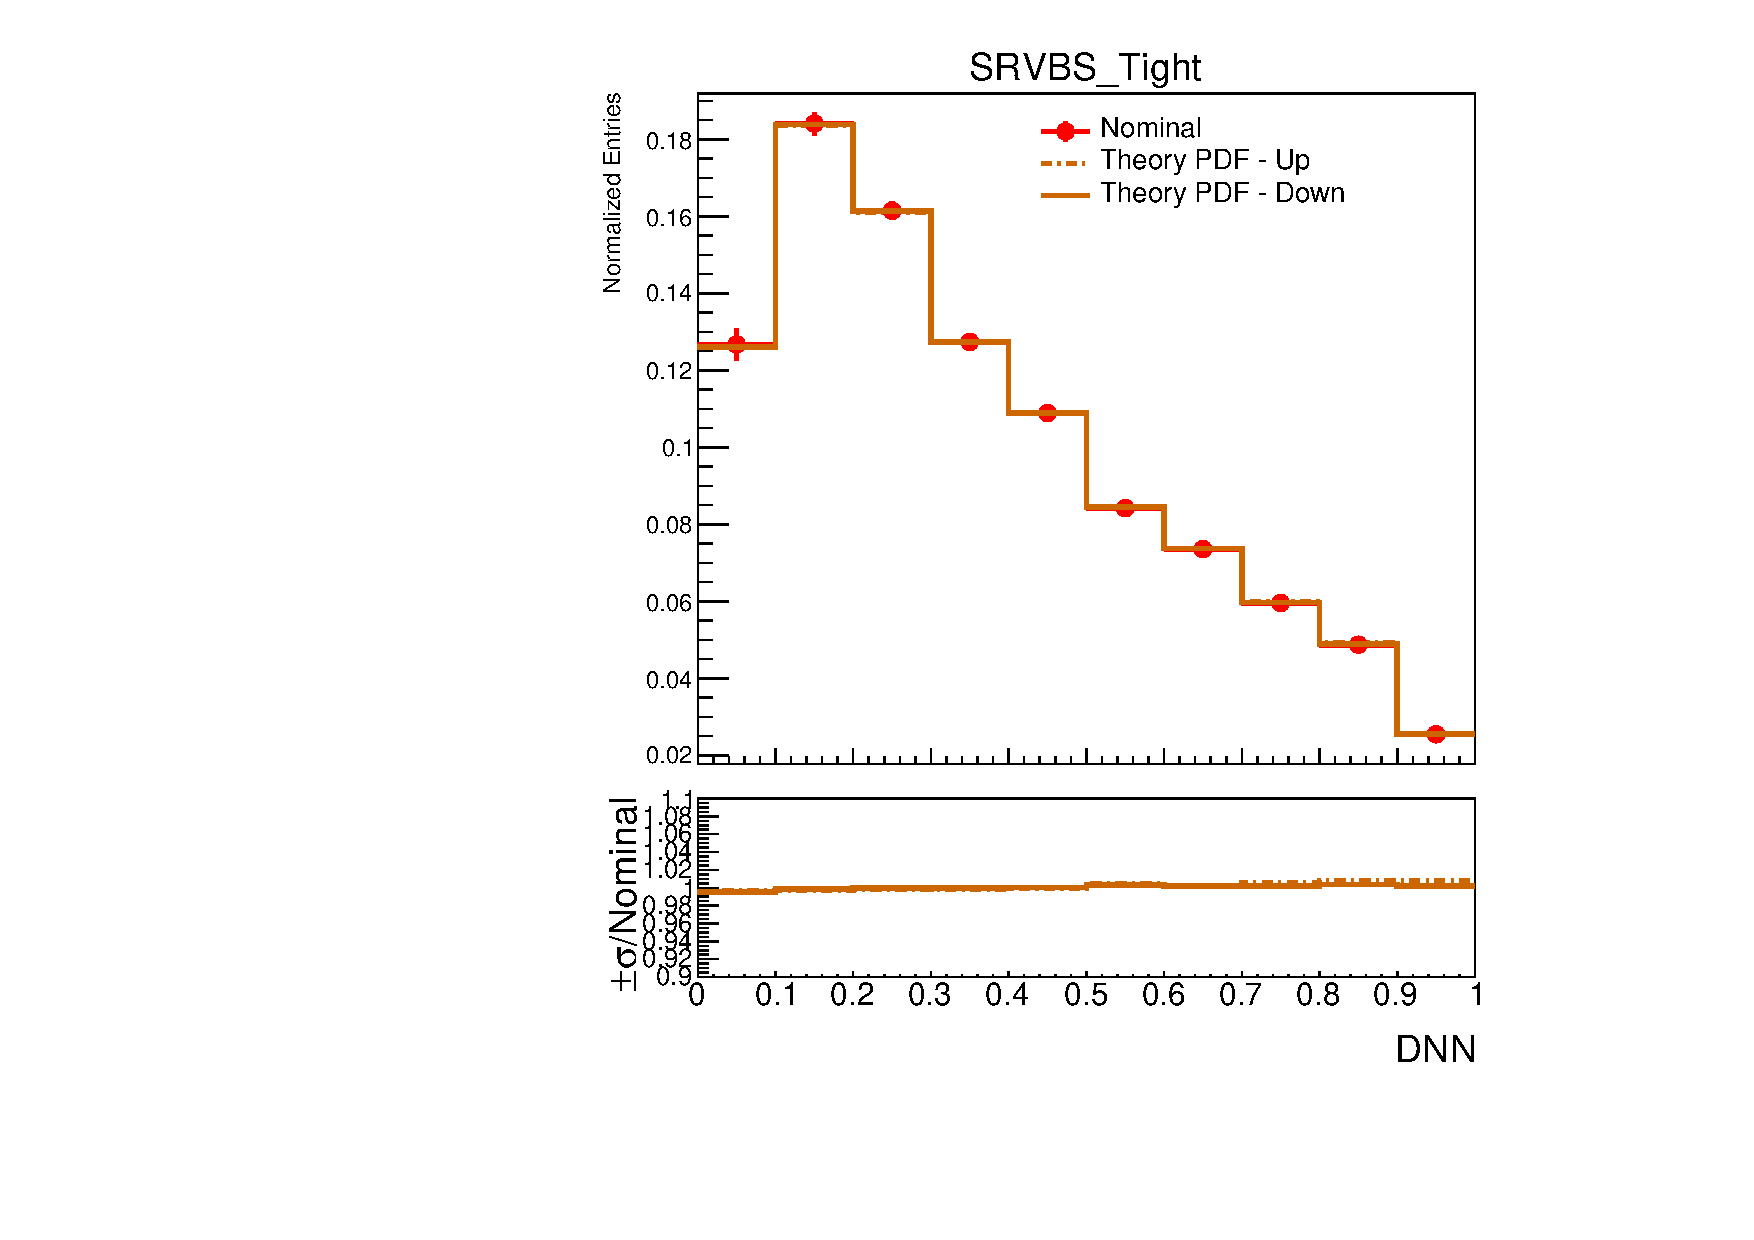
\includegraphics[width=\textwidth]{figures/1lep/PDFUnc/TheoryPDF/W_0ptag2pjet_0ptv_SRVBS_Tight_DNN_SysTheoryPDF_W__1up_Norm.pdf}
        \caption{\Wjets, resolved SR}
    \end{subfigure}
    \begin{subfigure}[b]{0.3\textwidth}
        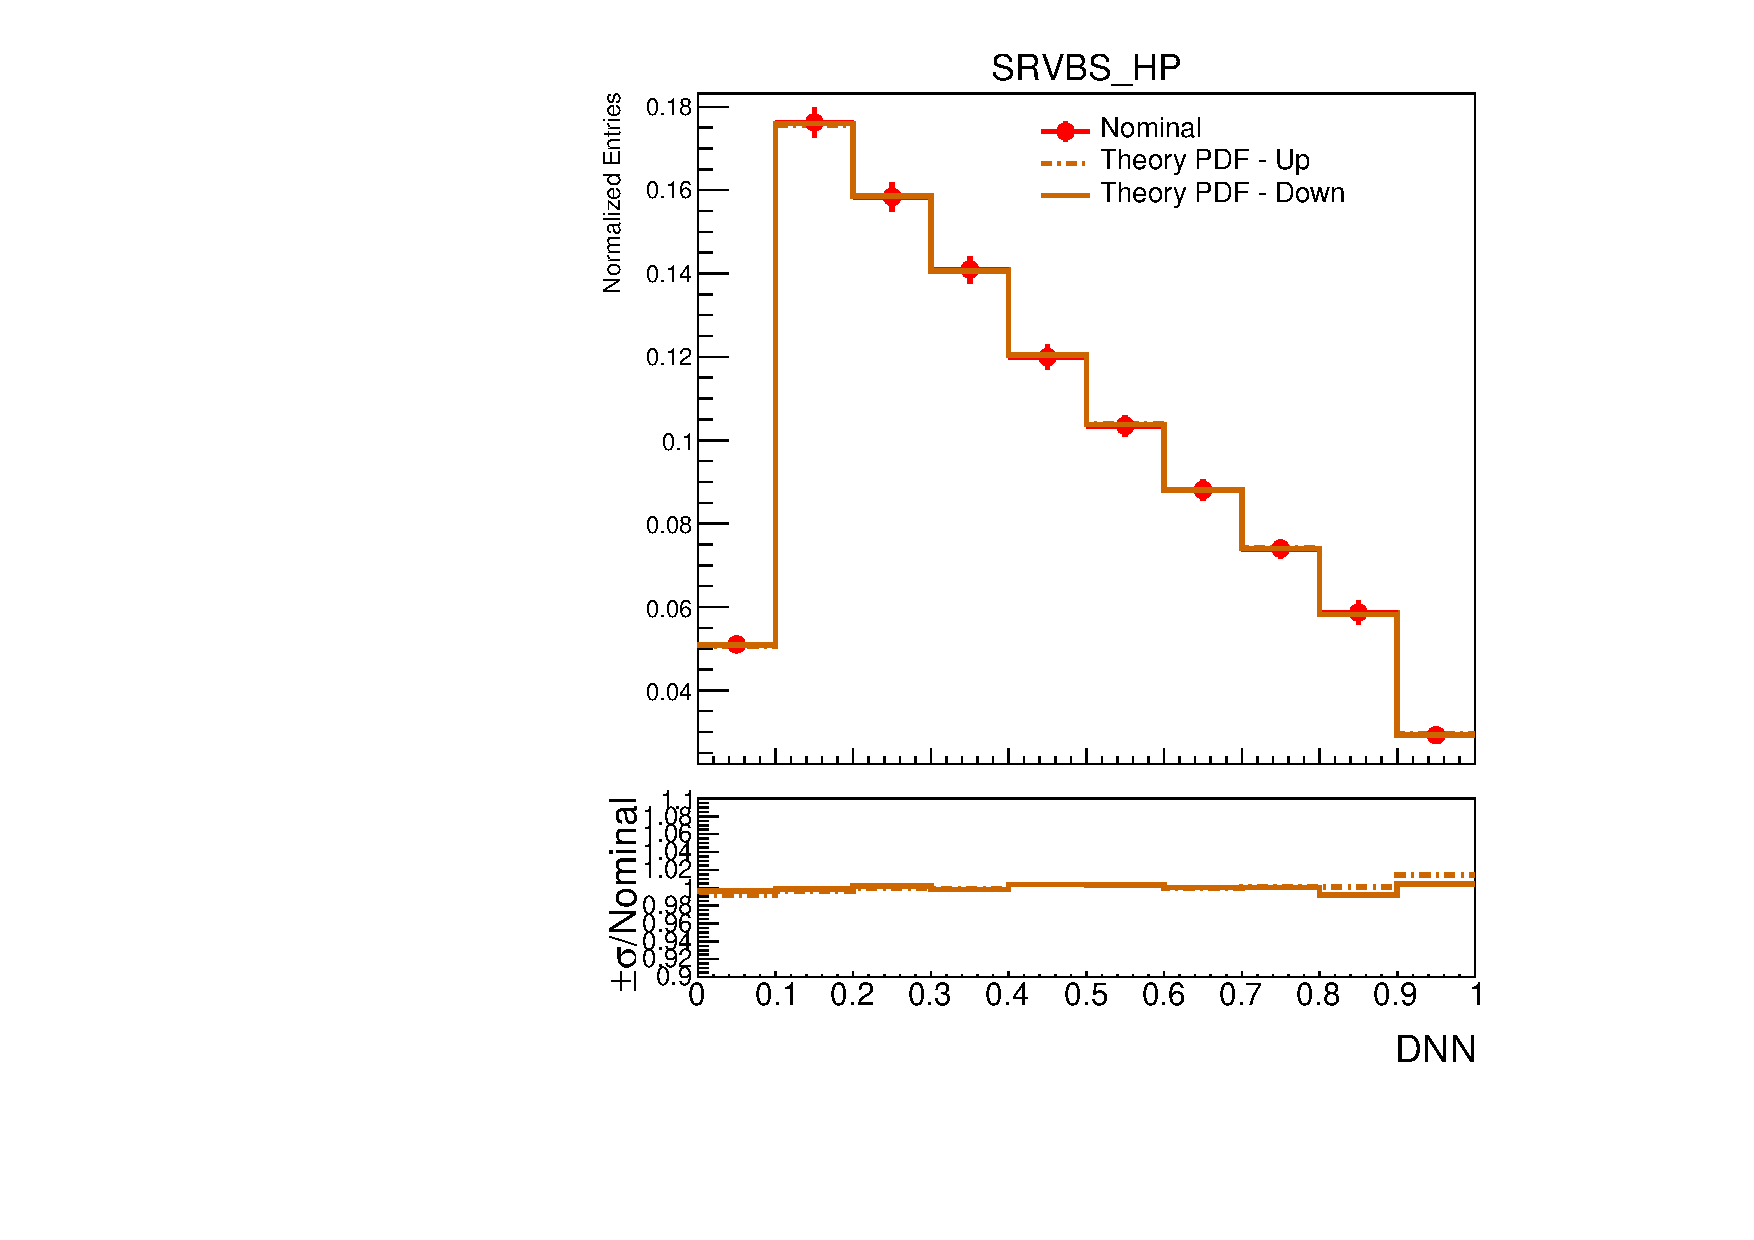
\includegraphics[width=\textwidth]{figures/1lep/PDFUnc/TheoryPDF/W_0ptag1pfat0pjet_0ptv_SRVBS_HP_DNN_SysTheoryPDF_W__1up_Norm.pdf}
        \caption{\Wjets, merged HP SR}
    \end{subfigure}
    \begin{subfigure}[b]{0.3\textwidth}
        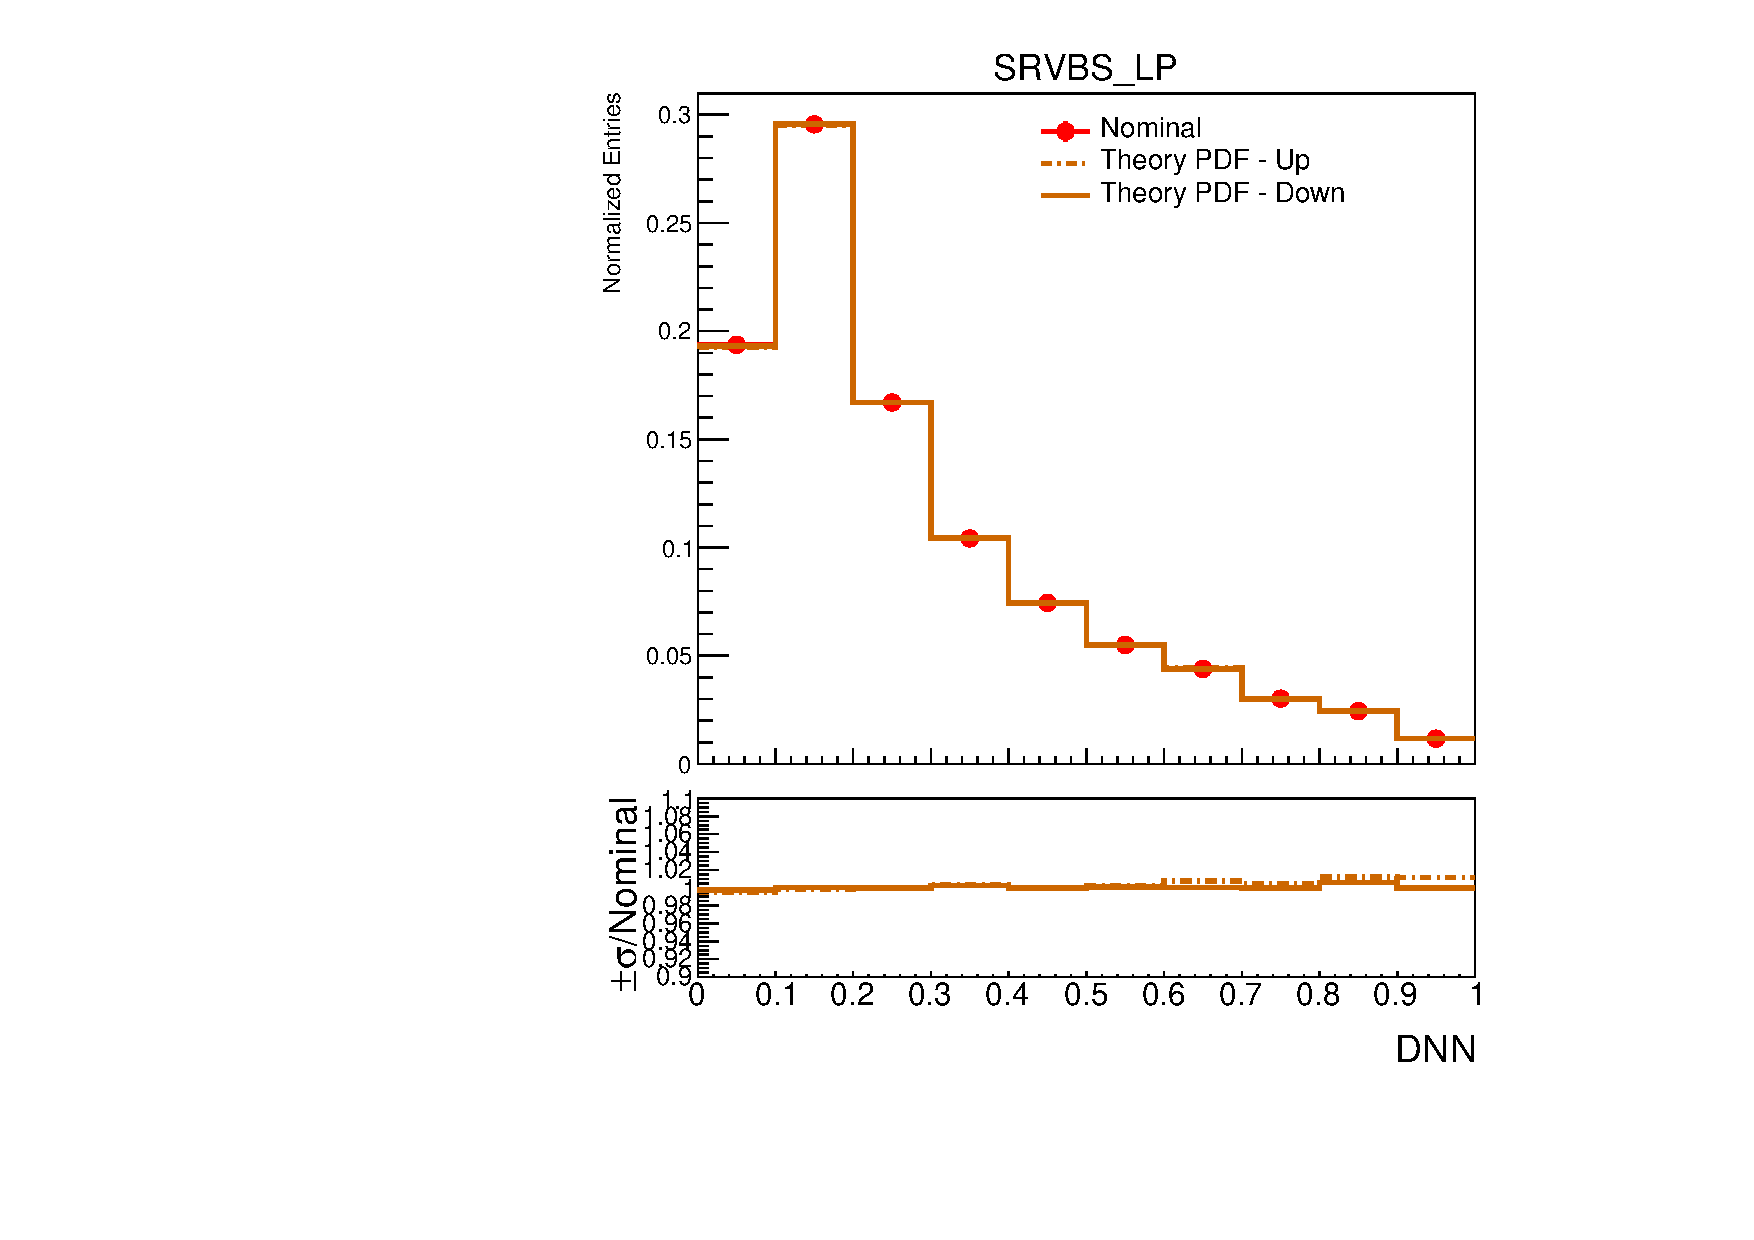
\includegraphics[width=\textwidth]{figures/1lep/PDFUnc/TheoryPDF/W_0ptag1pfat0pjet_0ptv_SRVBS_LP_DNN_SysTheoryPDF_W__1up_Norm.pdf}
        \caption{\Wjets, merged LP SR}
    \end{subfigure}
    \\
    \vspace{15mm}
    \begin{subfigure}[b]{0.3\textwidth}
        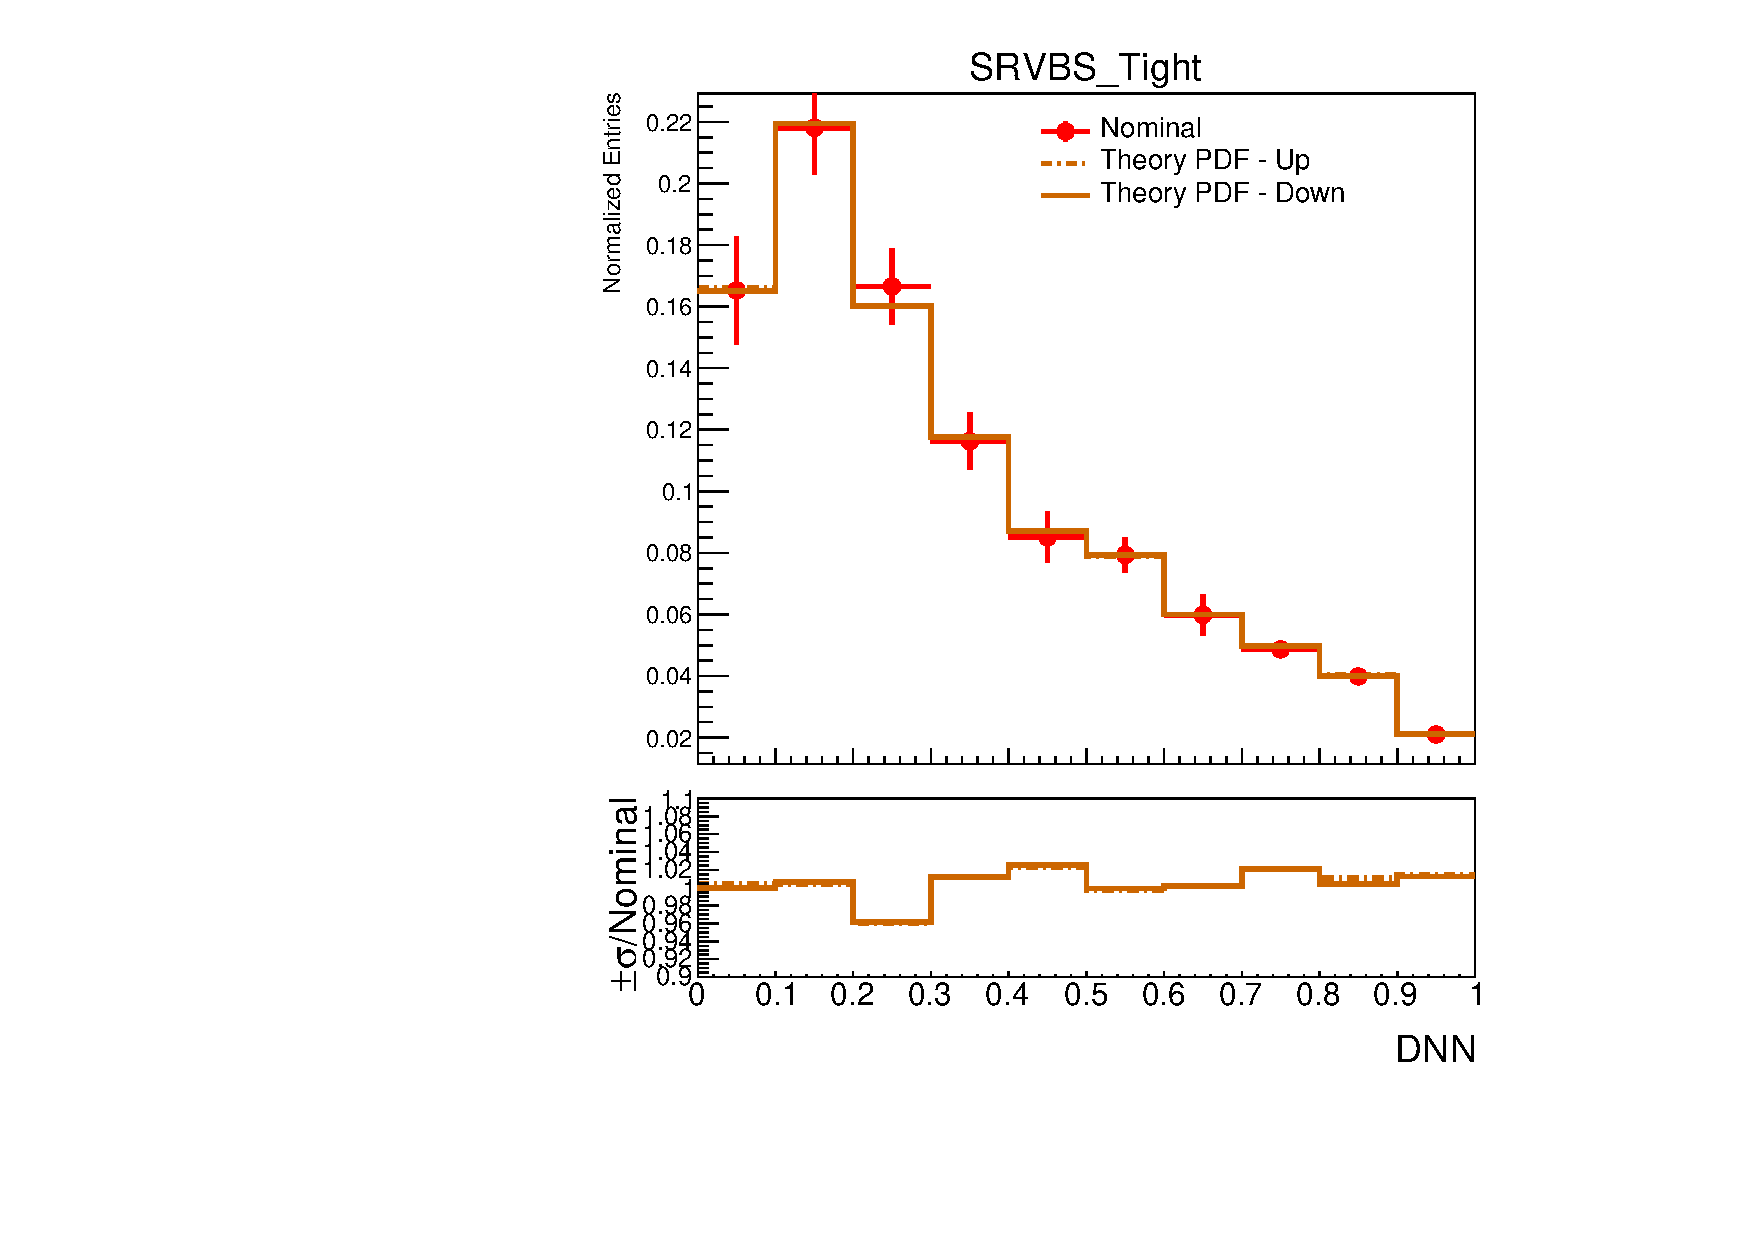
\includegraphics[width=\textwidth]{figures/1lep/PDFUnc/TheoryPDF/Z_0ptag2pjet_0ptv_SRVBS_Tight_DNN_SysTheoryPDF_Z__1up_Norm.pdf}
        \caption{\Zjets, resolved SR}
    \end{subfigure}
    \begin{subfigure}[b]{0.3\textwidth}
        \includegraphics[width=\textwidth]{figures/1lep/PDFUnc/TheoryPDF/Z_0ptag1pfat0pjet_0ptv_SRVBS_HP_DNN_SysTheoryPDF_Z__1up_Norm.pdf}
        \caption{\Zjets, merged HP SR}
    \end{subfigure}
    \begin{subfigure}[b]{0.3\textwidth}
        \includegraphics[width=\textwidth]{figures/1lep/PDFUnc/TheoryPDF/Z_0ptag1pfat0pjet_0ptv_SRVBS_LP_DNN_SysTheoryPDF_Z__1up_Norm.pdf}
        \caption{\Zjets, merged LP SR}
    \end{subfigure}
    \caption{Alternative PDF uncertainties in the 1-lepton channel. Histograms are normalized.}
    \label{fig:extPDFUnc1Lep}
\end{figure}


\begin{figure}[ht]
    \centering
    \begin{subfigure}[b]{0.3\textwidth}
        \includegraphics[width=\textwidth]{figures/1lep/PDFUnc/NNPDF/W_0ptag2pjet_0ptv_SRVBS_Tight_DNN_SysTheoryPDF_NNPDF_W__1up_Norm.pdf}
        \caption{\Wjets, resolved SR}
    \end{subfigure}
    \begin{subfigure}[b]{0.3\textwidth}
        \includegraphics[width=\textwidth]{figures/1lep/PDFUnc/NNPDF/W_0ptag1pfat0pjet_0ptv_SRVBS_HP_DNN_SysTheoryPDF_NNPDF_W__1up_Norm.pdf}
        \caption{\Wjets, merged HP SR}
    \end{subfigure}
    \begin{subfigure}[b]{0.3\textwidth}
        \includegraphics[width=\textwidth]{figures/1lep/PDFUnc/NNPDF/W_0ptag1pfat0pjet_0ptv_SRVBS_LP_DNN_SysTheoryPDF_NNPDF_W__1up_Norm.pdf}
        \caption{\Wjets, merged LP SR}
    \end{subfigure}
    \\
    \vspace{15mm}
    \begin{subfigure}[b]{0.3\textwidth}
        \includegraphics[width=\textwidth]{figures/1lep/PDFUnc/NNPDF/ttbar_0ptag2pjet_0ptv_SRVBS_Tight_DNN_SysTheoryPDF_NNPDF_ttbar__1up_Norm.pdf}
        \caption{\ttbar, resolved SR}
    \end{subfigure}
    \begin{subfigure}[b]{0.3\textwidth}
        \includegraphics[width=\textwidth]{figures/1lep/PDFUnc/NNPDF/ttbar_0ptag1pfat0pjet_0ptv_SRVBS_HP_DNN_SysTheoryPDF_NNPDF_ttbar__1up_Norm.pdf}
        \caption{\ttbar, merged HP SR}
    \end{subfigure}
    \begin{subfigure}[b]{0.3\textwidth}
        \includegraphics[width=\textwidth]{figures/1lep/PDFUnc/NNPDF/ttbar_0ptag1pfat0pjet_0ptv_SRVBS_LP_DNN_SysTheoryPDF_NNPDF_ttbar__1up_Norm.pdf}
        \caption{\ttbar, merged LP SR}
    \end{subfigure}
    \\
    \vspace{15mm}
    \begin{subfigure}[b]{0.3\textwidth}
        \includegraphics[width=\textwidth]{figures/1lep/PDFUnc/NNPDF/Z_0ptag2pjet_0ptv_SRVBS_Tight_DNN_SysTheoryPDF_NNPDF_Z__1up_Norm.pdf}
        \caption{\Zjets, resolved SR}
    \end{subfigure}
    \begin{subfigure}[b]{0.3\textwidth}
        \includegraphics[width=\textwidth]{figures/1lep/PDFUnc/NNPDF/Z_0ptag1pfat0pjet_0ptv_SRVBS_HP_DNN_SysTheoryPDF_NNPDF_Z__1up_Norm.pdf}
        \caption{\Zjets, merged HP SR}
    \end{subfigure}
    \begin{subfigure}[b]{0.3\textwidth}
        \includegraphics[width=\textwidth]{figures/1lep/PDFUnc/NNPDF/Z_0ptag1pfat0pjet_0ptv_SRVBS_LP_DNN_SysTheoryPDF_NNPDF_Z__1up_Norm.pdf}
        \caption{\Zjets, merged LP SR}
    \end{subfigure}
    \caption{PDF uncertainties using the NNPDF set in the 1-lepton channel. Histograms are normalized.}
    \label{fig:PDFUnc1Lep_bkg}
\end{figure}

\begin{figure}[ht]
    \centering
    \begin{subfigure}[b]{0.3\textwidth}
        \includegraphics[width=\textwidth]{figures/1lep/PDFUnc/QCDScale/W_0ptag2pjet_0ptv_SRVBS_Tight_DNN_SysTheoryQCD_W__1up_Norm.pdf}
        \caption{\Wjets, resolved SR}
    \end{subfigure}
    \begin{subfigure}[b]{0.3\textwidth}
        \includegraphics[width=\textwidth]{figures/1lep/PDFUnc/QCDScale/W_0ptag1pfat0pjet_0ptv_SRVBS_HP_DNN_SysTheoryQCD_W__1up_Norm.pdf}
        \caption{\Wjets, merged HP SR}
    \end{subfigure}
    \begin{subfigure}[b]{0.3\textwidth}
        \includegraphics[width=\textwidth]{figures/1lep/PDFUnc/QCDScale/W_0ptag1pfat0pjet_0ptv_SRVBS_LP_DNN_SysTheoryQCD_W__1up_Norm.pdf}
        \caption{\Wjets, merged LP SR}
    \end{subfigure}
    \\
    \vspace{15mm}
    \begin{subfigure}[b]{0.3\textwidth}
        \includegraphics[width=\textwidth]{figures/1lep/PDFUnc/QCDScale/ttbar_0ptag2pjet_0ptv_SRVBS_Tight_DNN_SysTheoryQCD_ttbar__1up_Norm.pdf}
        \caption{\ttbar, resolved SR}
    \end{subfigure}
    \begin{subfigure}[b]{0.3\textwidth}
        \includegraphics[width=\textwidth]{figures/1lep/PDFUnc/QCDScale/ttbar_0ptag1pfat0pjet_0ptv_SRVBS_HP_DNN_SysTheoryQCD_ttbar__1up_Norm.pdf}
        \caption{\ttbar, merged HP SR}
    \end{subfigure}
    \begin{subfigure}[b]{0.3\textwidth}
        \includegraphics[width=\textwidth]{figures/1lep/PDFUnc/QCDScale/ttbar_0ptag1pfat0pjet_0ptv_SRVBS_LP_DNN_SysTheoryQCD_ttbar__1up_Norm.pdf}
        \caption{\ttbar, merged LP SR}
    \end{subfigure}
    \\
    \vspace{15mm}
    \begin{subfigure}[b]{0.3\textwidth}
        \includegraphics[width=\textwidth]{figures/1lep/PDFUnc/QCDScale/Z_0ptag2pjet_0ptv_SRVBS_Tight_DNN_SysTheoryQCD_Z__1up_Norm.pdf}
        \caption{\Zjets, resolved SR}
    \end{subfigure}
    \begin{subfigure}[b]{0.3\textwidth}
        \includegraphics[width=\textwidth]{figures/1lep/PDFUnc/QCDScale/Z_0ptag1pfat0pjet_0ptv_SRVBS_HP_DNN_SysTheoryQCD_Z__1up_Norm.pdf}
        \caption{\Zjets, merged HP SR}
    \end{subfigure}
    \begin{subfigure}[b]{0.3\textwidth}
        \includegraphics[width=\textwidth]{figures/1lep/PDFUnc/QCDScale/Z_0ptag1pfat0pjet_0ptv_SRVBS_LP_DNN_SysTheoryQCD_Z__1up_Norm.pdf}
        \caption{\Zjets, merged LP SR}
    \end{subfigure}
    \caption{QCD scale uncertainties in the 1-lepton channel. Histograms are normalized.}
    \label{fig:PDFUnc1Lep_QCD}
\end{figure}

\clearpage
\subsection{ISR/FSR uncertainties}
\label{subsec:isr_fsr_unc}

The impact of initial and final state radiation (ISR/FSR) on top quark backgrounds is investigated using dedicated samples that vary the amount of additional radiation.
Figures \ref{fig:isrUnc1Lep} and \ref{fig:fsrUnc1Lep} illustrate the effects of these ISR and FSR uncertainties in the \olep channel.

%%%\begin{figure}[ht]
%%%    \centering
%%%    \begin{subfigure}[b]{0.3\textwidth}
%%%        \includegraphics[width=\textwidth]{figures/1lep/PDFUnc/FSR/ttbar_0ptag2pjet_0ptv_SRVBS_Tight_DNN_SysTheoryFSR_Top__1up_Norm.pdf}
%%%        \caption{\ttbar, resolved SR}
%%%    \end{subfigure}
%%%    \begin{subfigure}[b]{0.3\textwidth}
%%%        \includegraphics[width=\textwidth]{figures/1lep/PDFUnc/FSR/ttbar_0ptag1pfat0pjet_0ptv_SRVBS_HP_DNN_SysTheoryFSR_Top__1up_Norm.pdf}
%%%        \caption{\ttbar, merged HP SR}
%%%    \end{subfigure}
%%%    \begin{subfigure}[b]{0.3\textwidth}
%%%        \includegraphics[width=\textwidth]{figures/1lep/PDFUnc/FSR/ttbar_0ptag1pfat0pjet_0ptv_SRVBS_LP_DNN_SysTheoryFSR_Top__1up_Norm.pdf}
%%%        \caption{\ttbar, merged LP SR}
%%%    \end{subfigure}
%%%    \label{fig:fsrUnc1Lep}
%%%\end{figure}


\begin{figure}[htp]
    \centering
    \begin{subfigure}[b]{0.3\textwidth}
        \includegraphics[width=\textwidth]{figures/1lep/PDFUnc/ISR/ttbar_0ptag2pjet_0ptv_SRVBS_Tight_DNN_SysTheoryISR_ttbar__1up_Norm.pdf}
        \caption{\ttbar, resolved SR}
    \end{subfigure}
    \begin{subfigure}[b]{0.3\textwidth}
        \includegraphics[width=\textwidth]{figures/1lep/PDFUnc/ISR/ttbar_0ptag1pfat0pjet_0ptv_SRVBS_HP_DNN_SysTheoryISR_ttbar__1up_Norm.pdf}
        \caption{\ttbar, merged HP SR}
    \end{subfigure}
    \begin{subfigure}[b]{0.3\textwidth}
        \includegraphics[width=\textwidth]{figures/1lep/PDFUnc/ISR/ttbar_0ptag1pfat0pjet_0ptv_SRVBS_LP_DNN_SysTheoryISR_ttbar__1up_Norm.pdf}
        \caption{\ttbar, merged LP SR}
    \end{subfigure}
    \\
    \vspace{3mm}
    \begin{subfigure}[b]{0.3\textwidth}
        \includegraphics[width=\textwidth]{figures/1lep/PDFUnc/ISR/stop_0ptag2pjet_0ptv_SRVBS_Tight_DNN_SysTheoryISR_stop__1up_Norm.pdf}
        \caption{single top, resolved SR}
    \end{subfigure}
    \begin{subfigure}[b]{0.3\textwidth}
        \includegraphics[width=\textwidth]{figures/1lep/PDFUnc/ISR/stop_0ptag1pfat0pjet_0ptv_SRVBS_HP_DNN_SysTheoryISR_stop__1up_Norm.pdf}
        \caption{single top, merged HP SR}
    \end{subfigure}
    \begin{subfigure}[b]{0.3\textwidth}
        \includegraphics[width=\textwidth]{figures/1lep/PDFUnc/ISR/stop_0ptag1pfat0pjet_0ptv_SRVBS_LP_DNN_SysTheoryISR_stop__1up_Norm.pdf}
        \caption{single top, merged LP SR}
    \end{subfigure}
    \caption{ISR uncertainties in the 1-lepton channel.}
    \label{fig:isrUnc1Lep}
\end{figure}

\begin{figure}[htp]
    \centering
    \begin{subfigure}[b]{0.3\textwidth}
        \includegraphics[width=\textwidth]{figures/1lep/PDFUnc/FSR/ttbar_0ptag2pjet_0ptv_SRVBS_Tight_DNN_SysTheoryFSR_Top__1up_Norm.pdf}
        \caption{\ttbar, resolved SR}
    \end{subfigure}
    \begin{subfigure}[b]{0.3\textwidth}
        \includegraphics[width=\textwidth]{figures/1lep/PDFUnc/FSR/ttbar_0ptag1pfat0pjet_0ptv_SRVBS_HP_DNN_SysTheoryFSR_Top__1up_Norm.pdf}
        \caption{\ttbar, merged HP SR}
    \end{subfigure}
    \begin{subfigure}[b]{0.3\textwidth}
        \includegraphics[width=\textwidth]{figures/1lep/PDFUnc/FSR/ttbar_0ptag1pfat0pjet_0ptv_SRVBS_LP_DNN_SysTheoryFSR_Top__1up_Norm.pdf}
        \caption{\ttbar, merged LP SR}
    \end{subfigure}
    \caption{FSR uncertainties in the 1-lepton channel.}
    \label{fig:fsrUnc1Lep}
\end{figure}

%%%%%%%%
%\clearpage
\subsection{Tag Jets re-weighting}
\label{subsec:bkg_uncer_mjjrew}

As outlined in Section \ref{subsec:mjj_reweight}, a reweighting procedure is applied to the \Vjets samples based on the \mjjtag variable. 
An uncertainty is assigned to this reweighting by assuming a 100\% uncertainty in the parameters of the linear fit. 
This is treated as a modeling systematic uncertainty for both \Wjets\ and \Zjets backgrounds.



%
\clearpage
\section{Signal Uncertainties}
\clearpage
\subsection{Signal Uncertainties}
\label{subsec:sig_uncer}


\subsubsection{Scales and PDF uncertainties}
\label{subsec:sig_uncer_scales_PDF}

Additional systematic, as summarized below, are introduced due to modelling differences between various signal Monte Carlo generators.

\begin{itemize}
        \item QCD scale uncertainties (for signal samples generated at NLO QCD);
        \item PDF uncertainty;
\end{itemize}

Those uncertainties on the signal acceptance are included in the fit. They are studied by using truth weight information stored in the current analysis framework flow.

%Some additional scale uncertainties are available in our signal samples; in particular, they refer to some dynamic scale uncertainty obtained by changing the definition of the $\mu_0$. The three available choices:
%
%     \begin{itemize}
%        \item dyn\_scale\_choice\_HT
%        \item dyn\_scale\_choice\_sqrts
%        \item dyn\_scale\_choice\_sum\_pt
%    \end{itemize}

%are combined with the default uncertainties about the variation of the $\mu_f$. This choice has been made consistent with the strategy used here in \cite{Bittrich:2770539}; further information is also provided on the reference.

In particular, for the scale uncertainty we use the envelope of the usual 7 variations as for the background samples and described in Section \ref{subsec:scale_pdf_unc}.

Examples of these uncertaintiy are given in Figures \ref{fig:SigTheoUnc2Lep}-\ref{fig:ScaleUnc1Lep_sig}-\ref{fig:PDFUnc1Lep_sig}-\ref{fig:SigTheoUnc0Lep}.

%2lep
\begin{figure}[ht]
        \centering
    	\subfigure[qcd scale: Merged HP SR]{\includegraphics[width=0.32\textwidth]{figures/2lep/RNN/QCDScale/EW6llqq_0ptag1pfat0pjet_0ptv_SRVBS_HP_RNNScoreMerged_SysTheoryQCD_VBS__1up_Norm.pdf}}
        \subfigure[qcd scale: Merged LP SR]{\includegraphics[width=0.32\textwidth]{figures/2lep/RNN/QCDScale/EW6llqq_0ptag1pfat0pjet_0ptv_SRVBS_LP_RNNScoreMerged_SysTheoryQCD_VBS__1up_Norm.pdf}}
    	\subfigure[qcd scale: resolved SR]{\includegraphics[width=0.32\textwidth]{figures/2lep/RNN/QCDScale/EW6llqq_0ptag2pjet_0ptv_SRVBS_Fid_RNNScoreResolved_SysTheoryQCD_VBS__1up_Norm.pdf}}\\
    	\subfigure[pdf: Merged HP SR]{\includegraphics[width=0.32\textwidth]{figures/2lep/RNN/NNPDF/EW6llqq_0ptag1pfat0pjet_0ptv_SRVBS_HP_RNNScoreMerged_SysTheoryPDF_NNPDF_VBS__1up_Norm.pdf}}
        \subfigure[pdf: Merged LP SR]{\includegraphics[width=0.32\textwidth]{figures/2lep/RNN/NNPDF/EW6llqq_0ptag1pfat0pjet_0ptv_SRVBS_LP_RNNScoreMerged_SysTheoryPDF_NNPDF_VBS__1up_Norm.pdf}}
    	\subfigure[pdf: resolved SR]{\includegraphics[width=0.32\textwidth]{figures/2lep/RNN/NNPDF/EW6llqq_0ptag2pjet_0ptv_SRVBS_Fid_RNNScoreResolved_SysTheoryPDF_NNPDF_VBS__1up_Norm.pdf}}\\
        \caption{QCD scale and PDF uncertainties of the signal MC sample in the 2-lepton channel. Histograms are normalized.}
    \label{fig:SigTheoUnc2Lep}
\end{figure}

%1lep
\begin{figure}[ht]
    \centering
        %\subfigure[Wjets samples, resolved SR]{\includegraphics[width=0.3\textwidth]{figures/1lep/PDFUnc/PDFUncWSRRESRNNScoreResolved.png}}
        %\subfigure[Wjets samples, merged HP SR]{\includegraphics[width=0.3\textwidth]{figures/1lep/PDFUnc/PDFUncWSRHPRNNScoreMerged.png}}
	%\subfigure[Wjets samples, merged LP SR]{\includegraphics[width=0.3\textwidth]{figures/1lep/PDFUnc/PDFUncWSRLPRNNScoreMerged.png}}\\
        %\subfigure[ttbar samples, resolved SR]{\includegraphics[width=0.3\textwidth]{figures/1lep/PDFUnc/PDFUncttbarSRRESRNNScoreResolved.png}}
        %\subfigure[ttbar samples, merged HP SR]{\includegraphics[width=0.3\textwidth]{figures/1lep/PDFUnc/PDFUncttbarSRHPRNNScoreMerged.png}}
	%\subfigure[ttbar samples, merged LP SR]{\includegraphics[width=0.3\textwidth]{figures/1lep/PDFUnc/PDFUncttbarSRLPRNNScoreMerged.png}}\\
        \subfigure[signal samples, resolved SR]{\includegraphics[width=0.3\textwidth]{figures/1lep/PDFUnc/PDFUncEW6SRRESRNNScoreResolved.png}}
        \subfigure[signal samples, merged HP SR]{\includegraphics[width=0.3\textwidth]{figures/1lep/PDFUnc/PDFUncEW6SRHPRNNScoreMerged.png}}
	\subfigure[signal samples, merged LP SR]{\includegraphics[width=0.3\textwidth]{figures/1lep/PDFUnc/PDFUncEW6SRLPRNNScoreMerged.png}}
        \caption{Scale/Matrix uncertainties for 
%Wjets, ttbar, and 
signal samples in the signal regions, for the 1 lepton channel. Only events from MC16A campaign are shown here. Distributions are not normalized.}
    \label{fig:ScaleUnc1Lep_sig}
\end{figure}

\begin{figure}[ht]
    \centering
        %\subfigure[Wjets samples, resolved SR]{\includegraphics[width=0.3\textwidth]{figures/1lep/PDFUnc/PDFUncWSRRESRNNScoreResolvedPDF.png}}
        %\subfigure[Wjets samples, merged HP SR]{\includegraphics[width=0.3\textwidth]{figures/1lep/PDFUnc/PDFUncWSRHPRNNScoreMergedPDF.png}}
	%\subfigure[Wjets samples, merged LP SR]{\includegraphics[width=0.3\textwidth]{figures/1lep/PDFUnc/PDFUncWSRLPRNNScoreMergedPDF.png}}\\
        %\subfigure[ttbar samples, resolved SR]{\includegraphics[width=0.3\textwidth]{figures/1lep/PDFUnc/PDFUncttbarSRRESRNNScoreResolvedPDF.png}}
        %\subfigure[ttbar samples, merged HP SR]{\includegraphics[width=0.3\textwidth]{figures/1lep/PDFUnc/PDFUncttbarSRHPRNNScoreMergedPDF.png}}
	%\subfigure[ttbar samples, merged LP SR]{\includegraphics[width=0.3\textwidth]{figures/1lep/PDFUnc/PDFUncttbarSRLPRNNScoreMergedPDF.png}}\\
        \subfigure[signal samples, resolved SR]{\includegraphics[width=0.3\textwidth]{figures/1lep/PDFUnc/PDFUncEW6SRRESRNNScoreResolvedPDF.png}}
        \subfigure[signal samples, merged HP SR]{\includegraphics[width=0.3\textwidth]{figures/1lep/PDFUnc/PDFUncEW6SRHPRNNScoreMergedPDF.png}}
	\subfigure[signal samples, merged LP SR]{\includegraphics[width=0.3\textwidth]{figures/1lep/PDFUnc/PDFUncEW6SRLPRNNScoreMergedPDF.png}}
        \caption{PDF uncertainties for 
%Wjets, ttbar, and 
signal samples in the signal regions, for the 1 lepton channel. Only events from MC16A campaign are shown here. Distributions are normalized, and pdf variation names are suppressed for clarity. 
%For Wjets samples, a total of 104 pdf variations are shown; for ttbar samples, a total of 43 pdf variations are shown; for signal samples, 
A total of 100 pdf variations are shown. Currently no protection against large weight events were applied, and the rare bin fluctuations are expected to be suppressed with a weight protection in place.}
    \label{fig:PDFUnc1Lep_sig}
\end{figure}

%0lep
\begin{figure}[ht]
        \centering
    	\subfigure[qcd scale: Merged HP SR]{\includegraphics[width=0.32\textwidth]{figures/0lep/systematics/systs/merged/plots/systqcdscaleSigsig_RNN_SRVBS_HP.pdf}}
        \subfigure[qcd scale: Merged LP SR]{\includegraphics[width=0.32\textwidth]{figures/0lep/systematics/systs/merged/plots/systqcdscaleSigsig_RNN_SRVBS_LP.pdf}}
    	\subfigure[qcd scale: resolved SR]{\includegraphics[width=0.32\textwidth]{figures/0lep/systematics/systs/merged/plots/systqcdscaleSigsig_RNN_SRVBS_Fid.pdf}}\\
    	\subfigure[pdf: Merged HP SR]{\includegraphics[width=0.32\textwidth]{figures/0lep/systematics/systs/merged/plots/systinternalpdfSigsig_RNN_SRVBS_HP.pdf}}
        \subfigure[pdf: Merged LP SR]{\includegraphics[width=0.32\textwidth]{figures/0lep/systematics/systs/merged/plots/systinternalpdfSigsig_RNN_SRVBS_LP.pdf}}
    	\subfigure[pdf: resolved SR]{\includegraphics[width=0.32\textwidth]{figures/0lep/systematics/systs/merged/plots/systinternalpdfSigsig_RNN_SRVBS_Fid.pdf}}\\
        \caption{QCD scale and PDF uncertainties of the signal MC sample in the 0-lepton channel}
    \label{fig:SigTheoUnc0Lep}
\end{figure}


\clearpage
\subsubsection{EWK-QCD interference}
\label{subsec:sig_uncer_interf}

As discussed in Section \ref{sec:mc_sample},
EWK and QCD VV+jj samples are generated seprately, therefore, no interference contribution is included.
The actual SM process is, indeed, given by:

\begin{equation}
    \begin{split}
        | M_{SM}(VV+jj) |^2 = | M_{QCD}(VV+jj) + M_{EWK}(VV+jj) |^2 =
                        \\ = |M_{QCD}(VV+jj)|^2 + |M_{EWK}(VV+jj)|^2 + |M_{Int}(VV+jj)|^2
    \end{split}
\end{equation}

In order to estimate the impact of such approximation dedicated (private) samples have been produced
for the inclusive $M_{SM}(VV+jj)$ as well as for the QCD one $M_{QCD}(VV+jj)$; 
this has been done for each of the lepton channel and for the allowed $WW, WZ, ZZ$ boson pairs.

Table \ref{tab:EWKQCDInt_xSec} is summarising the cross section of all the processes according to MG calculation:

\begin{table}[h]
    \centering
    \begin{tabular}{c|c|c|c} 
    \hline 
        Channel              & Inclusive   &  QCD      &    EWK \\    
    \hline 
        ZZ llqq              & $0.2375 \pm 5 \cdot 10^{-4}$  &  $0.2279 \pm 6 \cdot 10^{-4}$    &    $0.00989 \pm 1 \cdot 10^{-5}$\\    
        ZW llqq              & $0.580  \pm 1 \cdot 10^{-3}$  &  $0.536  \pm 1 \cdot 10^{-3}$    &    $0.0461 \pm 1 \cdot 10^{-4}$\\    
        
        WW lvqq              & $209.4 \pm 0.6$    &  $208.4 \pm 0.5$       &    $1.9994 + 1.9777$\\    
        WZ lvqq              & $3.172 \pm 8 \cdot 10^{-3}$  &  $2.921 \pm 6 \cdot 10^{-3}$     &    $0.2600 \pm 6 \cdot 10^{-4}$\\    

        ZZ vvqq              & $0.848 \pm 2 \cdot 10^{-3}$  &  $0.816 \pm 2 \cdot 10^{-3}$     &    $0.03 \pm 8 \cdot 10^{-2}$\\    
        ZW vvqq              & $2.049 \pm 6 \cdot 10^{-3}$  &  $1.892 \pm 4 \cdot 10^{-3}$     &    $0.1572 \pm 5 \cdot 10^{-4}$\\    

    \hline
    \end{tabular}
    \caption{Cross section of the Inclusive, QCD and EWK components of the SM VV+jj production. Note that for WW lvqq sample we rely on baseline EWK samples and the cross sections as reported in Section \ref{sec:mc_sample_ewvvjj}.}
    \label{tab:EWKQCDInt_xSec}
  \end{table}


In this way, an estimation of the interference term can be evaluated as follow:

\begin{equation}
    |M_{Int}(VV+jj)|^2 = | M_{SM}(VV+jj) |^2 - |M_{QCD}(VV+jj)|^2 - |M_{EWK}(VV+jj)|^2
\end{equation}

in particular, since reconstructed level samples are not available for these processes,
we evaluated the impact of such term in the fiducial SRs of the analysis as defined 
in Section \ref{subsec:fidbin_definition}.

Figure \ref{fig:EWKQCDInt_Mjj_0lep}, \ref{fig:EWKQCDInt_Mjj_1lep} and \ref{fig:EWKQCDInt_Mjj_2lep}
show the distribution of the Truth \mjjtag for the \zlep, \olep and \tlep channels 
%l(\textcolor{red}{note: one sample for the \olep channel is currently stucking on the grid, plots will be added later})
.

\begin{figure}[ht]
    \centering
        \subfigure[\zlep - Resolved]{\includegraphics[width=0.45\textwidth]{figures/EWKQCDInt/plot_TagJJM_SR_0lep_Resolved.pdf}}
        \subfigure[\zlep - Merged]{\includegraphics[width=0.45\textwidth]{figures/EWKQCDInt/plot_TagJJM_SR_0lep_Merged.pdf}}
    \caption{Impact of the EWK-QCD interference term on the \mjjtag distribution in \zlep channel for 
                the fiducial Resolved SR (left) and Merged SR (right).}
    \label{fig:EWKQCDInt_Mjj_0lep}
\end{figure}

\begin{figure}[ht]
    \centering
        \subfigure[\olep - Resolved]{\includegraphics[width=0.45\textwidth]{figures/EWKQCDInt/plot_TagJJM_SR_1lep_Resolved.pdf}}
        \subfigure[\olep - Merged]{\includegraphics[width=0.45\textwidth]{figures/EWKQCDInt/plot_TagJJM_SR_1lep_Merged.pdf}}
    \caption{Impact of the EWK-QCD interference term on the \mjjtag distribution in \olep channel for 
                the fiducial Resolved SR (left) and Merged SR (right).}
    \label{fig:EWKQCDInt_Mjj_1lep}
\end{figure}

\begin{figure}[ht]
    \centering
        \subfigure[\tlep - Resolved]{\includegraphics[width=0.45\textwidth]{figures/EWKQCDInt/plot_TagJJM_SR_2lep_Resolved.pdf}}
        \subfigure[\tlep - Merged]{\includegraphics[width=0.45\textwidth]{figures/EWKQCDInt/plot_TagJJM_SR_2lep_Merged.pdf}}
    \caption{Impact of the EWK-QCD interference term on the \mjjtag distribution in \tlep channel for 
                the fiducial Resolved SR (left) and Merged SR (right).}
    \label{fig:EWKQCDInt_Mjj_2lep}
\end{figure}

Since the interference term is found not negligible, a shape uncertainty can be evaluated considering 
the ratio $(EWK+Int) / EWK$ as shown in the ratio pannel of the plots.
In particular, the $max(|R-1|, \Delta R)$ is used as input to build the variations, where R is the ratio
$(EWK+Int) / EWK$ and the $\Delta R$ is the uncertainty on it, as shown in table \ref{tab:IntUnc}.

\begin{landscape}
\begin{table}[h]
    \begin{center} 
    \begin{tabular}{c|c|c|c|c|c|c|c|c|c|c} 
    \hline 
        $(EWK+Int)/EWK$         & & \multicolumn{3}{c|}{\zlep}   & \multicolumn{3}{c|}{ \olep} & \multicolumn{3}{c}{ \tlep} \\    
                                & & R	    &DR	    & max(|R-1|, DR)    & R	    &DR	    & max(|R-1|, DR)    & R	    &DR	    & max(|R-1|, DR) \\
    \hline 
        \multirow{3}{*}{Merged SR}      & 1st bin   & 1,055	& 0,131	& 0,131	& 0,747	& 0,251	& 0,253	& 0,919	& 0,049	& 0,081 \\
                                        & 2nd bin   & 0,956	& 0,096	& 0,096	& 1,122	& 0,184	& 0,184	& 0,999	& 0,041	& 0,041 \\
                                        & 3rd bin   & 0,835	& 0,063	& 0,165	& 1,085	& 0,117	& 0,117	& 0,976	& 0,030	& 0,030 \\
        \multirow{3}{*}{Resolved SR}    & 1st bin   & 0,979	& 0,095	& 0,095	& 1,213	& 0,153	& 0,213	& 0,910	& 0,040	& 0,090 \\
                                        & 2nd bin   & 0,996	& 0,054	& 0,054	& 1,090	& 0,088	& 0,090	& 0,889	& 0,025	& 0,111 \\
                                        & 3rd bin   & 1,012	& 0,034	& 0,034	& 1,091	& 0,054	& 0,091	& 0,924	& 0,018	& 0,076 \\

    \hline
    \end{tabular}
    \caption{Interference uncertainty as a function of the \mjjtag variable for merged and resolved SRs and for each of the lepton channel.}
    \label{tab:IntUnc}
    \end{center} 
  \end{table}
\end{landscape}




The final discriminant model expects the tracks multiplicity of the small-R jets
as input variables and this is a pure reconstruction level information; 
in principle, the tracks multiplicity of the jets is, in first approximation, depending 
only on the $\pt$ and $\eta$ of the jets, so, it could be parametrised in such way
(like performing a DNN or GaussianProcess regression).
To avoid introducing further complexities and to not delay further the timescale of the analysis
we decided to keep the shape parametrisation of the interference term as function of the \mjjtag.
Indeed, this variable is well describing the dependency of the signal phase space
that the final discriminant learnt, as shown in Appendix \ref{app:rnn_2d}.

The final impact of such effect on the shape of the final discriminant at the reconstruction level
SRs is shown in Figure \ref{fig:EWQCDinput_bis}.

\begin{figure}[ht]
    \centering
     \subfigure[Resolved SR]{\includegraphics[width=0.46\textwidth]{figures/EWQCDint/EW6llqq_0ptag2pjet_0ptv_SRVBS_Fid_RNNScoreResolved_SysEWQCDint.pdf}}
     \subfigure[Merged HP SR]{\includegraphics[width=0.46\textwidth]{figures/EWQCDint/EW6llqq_0ptag1pfat0pjet_0ptv_SRVBS_HP_RNNScoreMerged_SysEWQCDint.pdf}}
     \caption{EW-QCD interference systematics uncertainty compared to the nominal distribution, used as input for the fitting.}
     \label{fig:EWQCDinput_bis}
\end{figure}

This uncertainty is used in the final fit model of the analysis 
and the impact of that is documented in Appendix \ref{app:EWQCDint}.



%%% shower uncertainty %%%
\clearpage
\subsubsection{Shower uncertainty}
\label{subsec:sig_uncer_shower}

The impact of the shower on the monte carlo samples generation is included in the final results
as uncertainty on the signal samples.
As mentioned in Section \ref{sec:mc_sample_ewvvjj}, 
dedicated alternative samples have been used for the full set of EWK VV+jj signal samples 
used in the analysis; these samples include Herwig instead of Pythia for the showering effects
and the validation is documented in Appendix \ref{app:H7Gen}.

The impact of the shower effect on both the shape and the normalisation
of the final discriminant is shown in Figures \ref{fig:Shower_SRs}-\ref{fig:Shower_CRs}
for the SRs and CRs respectively.

%%% SRs
\begin{figure}[ht]
    \centering
     \subfigure[\zlep - MergedHP SR]{\includegraphics[width=0.3\textwidth]{figures/ShowerUnc/valid/0lep/SR_HP.pdf}}
     \subfigure[\zlep - MergedLP SR]{\includegraphics[width=0.3\textwidth]{figures/ShowerUnc/valid/0lep/SR_LP.pdf}}
     \subfigure[\zlep - Resolved SR]{\includegraphics[width=0.3\textwidth]{figures/ShowerUnc/valid/0lep/SR_Tight.pdf}} \\
     \subfigure[\olep - MergedHP SR]{\includegraphics[width=0.3\textwidth]{figures/ShowerUnc/valid/1lep/SR_HP.pdf}}
     \subfigure[\olep - MergedLP SR]{\includegraphics[width=0.3\textwidth]{figures/ShowerUnc/valid/1lep/SR_LP.pdf}}
     \subfigure[\olep - Resolved SR]{\includegraphics[width=0.3\textwidth]{figures/ShowerUnc/valid/1lep/SR_Tight.pdf}} \\
     \subfigure[\tlep - MergedHP SR]{\includegraphics[width=0.3\textwidth]{figures/ShowerUnc/valid/2lep/SR_HP.pdf}}
     \subfigure[\tlep - MergedLP SR]{\includegraphics[width=0.3\textwidth]{figures/ShowerUnc/valid/2lep/SR_LP.pdf}}
     \subfigure[\tlep - Resolved SR]{\includegraphics[width=0.3\textwidth]{figures/ShowerUnc/valid/2lep/SR_Tight.pdf}} \\
     \caption{[SRs] Shower systematics uncertainty compared to the nominal distribution, used as input for the fitting.}
     \label{fig:Shower_SRs}
\end{figure}

%%% CRs
\begin{figure}[ht]
    \centering
     \subfigure[\zlep - Merged CR]{\includegraphics[width=0.3\textwidth]{figures/ShowerUnc/valid/0lep/CR_Merged.pdf}}
     \subfigure[\olep - Merged CR]{\includegraphics[width=0.3\textwidth]{figures/ShowerUnc/valid/1lep/CR_Merged.pdf}}
     \subfigure[\tlep - Merged CR]{\includegraphics[width=0.3\textwidth]{figures/ShowerUnc/valid/2lep/CR_Merged.pdf}} \\
     \subfigure[\zlep - Resolved CR]{\includegraphics[width=0.3\textwidth]{figures/ShowerUnc/valid/0lep/CR_Tight.pdf}}
     \subfigure[\olep - Resolved CR]{\includegraphics[width=0.3\textwidth]{figures/ShowerUnc/valid/1lep/CR_Tight.pdf}}
     \subfigure[\tlep - Resolved CR]{\includegraphics[width=0.3\textwidth]{figures/ShowerUnc/valid/2lep/CR_Tight.pdf}} \\
     \subfigure[\olep - MergedHP TopCR]{\includegraphics[width=0.3\textwidth]{figures/ShowerUnc/valid/1lep/CRTop_HP.pdf}}
     \subfigure[\olep - MergedLP TopCR]{\includegraphics[width=0.3\textwidth]{figures/ShowerUnc/valid/1lep/CRTop_LP.pdf}}
     \subfigure[\olep - Resolved TopCR]{\includegraphics[width=0.3\textwidth]{figures/ShowerUnc/valid/1lep/CRTop_Tight.pdf}}
     \caption{[CRs] Shower systematics uncertainty compared to the nominal distribution, used as input for the fitting.}
     \label{fig:Shower_CRs}
\end{figure}


